\chapter{Transition rates}\label{chap:2}

About $10^8$ dark-matter particles of \SI{100}{MeV} cross each square centimeter of a detector every second (\cref{we:1-flux}), each with at most \SI{350}{eV} of kinetic energy (\cref{sec:1.3}), and \cref{eq:1.5-rate} turns them into an event rate that \cref{chap:1} quoted without derivation. Deriving it is a question for quantum mechanics: how often does a weak interaction move a kilogram of silicon, with some $10^{26}$ electrons, from its ground state into one of its excited states? Scattering theory for two particles in vacuum answers only part of it, because a solid is not a free electron. Its excited states are states of many identical electrons, some of them can be reached only through an intermediate state that a phonon completes, and at any finite temperature the crystal can also hand energy back to the dark matter. Bosonic dark matter raises a related question, why its absorption rate depends on the local density and not on the flux. The answers need Fermi's golden rule and four extensions of it: the Born approximation, second quantization, second-order perturbation theory and the thermal average. With them we derive the cross-sections and form factors behind the reference quantities of \cref{sec:1.4}; \cref{fig:2-map} shows how each extends the golden rule.

\begin{figure}[tbp]
  \centering
  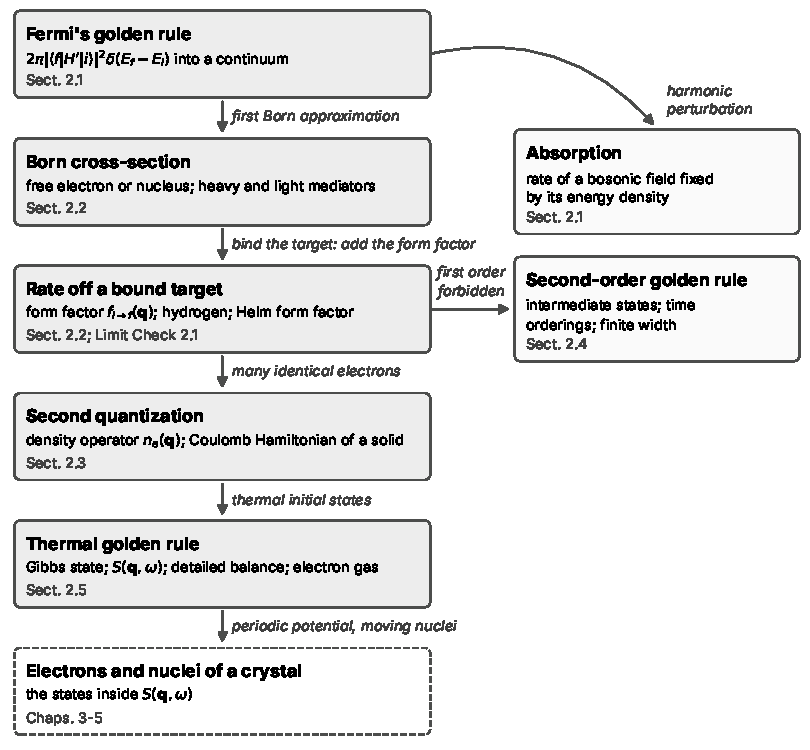
\includegraphics[width=0.85\linewidth]{figures/ch02/map02.pdf}
  \caption{From Fermi's golden rule to the dynamic structure factor. Arrows name the step between levels: the first Born approximation gives the cross-section on a free electron or nucleus (\cref{sec:2.1,sec:2.2}); binding the target adds the transition form factor $f_{i\to f}(\vect{q})$, checked on the ionization of hydrogen (\cref{sec:2.2}; \cref{lim:2.2a}); identical electrons call for occupation numbers and the density operator $n_e(\vect{q})$ (\cref{sec:2.3}); thermal initial states turn the rate into the dynamic structure factor $S(\vect{q},\omega)$ with detailed balance (\cref{sec:2.5}). Side branches: a harmonic perturbation gives the absorption rate of a bosonic field, set by its energy density (\cref{sec:2.1}), and a transition forbidden at first order proceeds through an intermediate state (\cref{sec:2.4}). The dashed box is the crystal whose states fill $S$ (\cref{chap:3,chap:4,chap:5}).}
  \label{fig:2-map}
\end{figure}

\section{Fermi's golden rule}\label{sec:2.1}

A kilogram of silicon exposed for a year to \SI{100}{MeV} dark matter with $\sigmae = \SI{e-40}{cm^2}$ expects 73 events in the toy rate of \cref{we:1-limit}, and twice as many in two years: the count is a rate times an exposure (\cref{eq:1.5-Nsig}). Quantum mechanics gives probabilities, not rates. A probability that grows linearly in time appears only when a weak perturbation couples an initial state to a continuum of final states, and only within a window of times. The derivation of Fermi's golden rule follows Refs.~\cite[Chap.~5]{sakurai2017modern} and \cite[Chap.~XIII]{cohentannoudji1977quantum}.

\subsection{First-order amplitude}

The target, together with a dark-matter particle far from it, evolves under an unperturbed Hamiltonian $H_0$ with eigenstates $|n\rangle$ and energies $E_n$. At $t = 0$ a perturbation $H'(t)$ is switched on, and the system starts in the eigenstate $|i\rangle$. We expand the state in the unperturbed basis, with the free phases taken out:
\begin{equation*}
  |\psi(t)\rangle = \sum_n c_n(t)\,\ee^{-\ii E_n t}\,|n\rangle, \qquad c_n(0) = \delta_{ni}.
\end{equation*}
Inserting this into $\ii\,\partial_t|\psi\rangle = (H_0 + H')|\psi\rangle$, the time derivative of each phase cancels the action of $H_0$. Projecting onto $\ee^{-\ii E_f t}|f\rangle$ leaves an exact set of equations for the amplitudes,
\begin{equation}
  \ii\,\dot c_f(t) = \sum_n \langle f|H'(t)|n\rangle\,\ee^{\ii(E_f - E_n)t}\,c_n(t).
  \label{eq:2.1-exact}
\end{equation}
To first order in $H'$ we replace $c_n(t)$ on the right by its initial value $\delta_{ni}$ and integrate. For $f \neq i$,
\begin{equation}
  c_f(t) = -\ii\int_0^t \dd t'\,\langle f|H'(t')|i\rangle\,\ee^{\ii(E_f - E_i)t'} ,
  \label{eq:2.1-c1}
\end{equation}
and the transition probability is $P_{i\to f}(t) = |c_f(t)|^2$. The replacement is consistent only while the initial state is barely depleted, $\sum_{f\neq i}P_{i\to f}(t) \ll 1$. \Cref{eq:2.1-c1} is the first term of the Dyson series of the interaction picture; \cref{sec:2.4} takes the second.

\subsection{Constant perturbation}

Let $H'$ be independent of time for $t > 0$. This is the case of dark-matter scattering: the interaction $H_{\mathrm{int}}$ does not depend on time, and energy passes between the dark matter and the target, whose kinetic and internal energies are both in $E_i$ and $E_f$. With $\xi = E_f - E_i$ the integral in \cref{eq:2.1-c1} is elementary, $c_f(t) = -\langle f|H'|i\rangle(\ee^{\ii\xi t} - 1)/\xi$. Since $|\ee^{\ii\xi t} - 1|^2 = 2 - 2\cos\xi t = 4\sin^2(\xi t/2)$,
\begin{equation}
  P_{i\to f}(t) = 4\,|\langle f|H'|i\rangle|^2\,\frac{\sin^2(\xi t/2)}{\xi^2} .
  \label{eq:2.1-Pstatic}
\end{equation}

All the time dependence sits in the function $\sin^2(\xi t/2)/\xi^2$, drawn in \cref{fig:2-golden}(a). At $\xi = 0$ it equals $t^2/4$. Its zeros are at $\xi = 2\pi k/t$ with $k$ a nonzero integer, so the central peak has width $4\pi/t$. The substitution $u = \xi t/2$ gives its integral,
\begin{equation*}
  \int_{-\infty}^{\infty}\dd\xi\,\frac{\sin^2(\xi t/2)}{\xi^2} = \frac{t}{2}\int_{-\infty}^{\infty}\dd u\,\frac{\sin^2 u}{u^2} = \frac{\pi t}{2} ,
\end{equation*}
with $\int\dd u\,\sin^2u/u^2 = \pi$ (\cref{app:C.1}). The height grows as $t^2$, the width shrinks as $1/t$, and the area grows as $t$; the central peak holds \SI{90.3}{\percent} of it. Integrated against any function $w(\xi)$ that varies little over a range $2\pi/t$, the function returns $(\pi t/2)\,w(0)$, with a relative error $\sim 1/(t\,\Delta_{\mathrm{w}})$, where $\Delta_{\mathrm{w}}$ is the range over which $w$ varies. In the sense of distributions,
\begin{equation}
  \frac{\sin^2(\xi t/2)}{\xi^2} \;\longrightarrow\; \frac{\pi t}{2}\,\delta(\xi) \qquad (t \to \infty) ,
  \label{eq:2.1-deltalimit}
\end{equation}
which \cref{app:C.1} proves. Applied to \cref{eq:2.1-Pstatic}, it gives a probability that grows linearly in time, $P_{i\to f}(t) \to 2\pi t\,|\langle f|H'|i\rangle|^2\,\delta(E_f - E_i)$. The same limit can be taken after differentiating. The time derivative of \cref{eq:2.1-Pstatic} is $2|\langle f|H'|i\rangle|^2\sin(\xi t)/\xi$, a function of $\xi$ whose area is $\pi$ at every $t > 0$ and whose width shrinks as $1/t$; it tends to $\pi\delta(\xi)$. Since the area stays fixed while the width shrinks, the probability per unit time stops depending on $t$, and that is what we mean by a rate. The transition rate is
\begin{keyresult}[Fermi's golden rule]
\begin{equation}
  \varGamma_{i\to f} = 2\pi\,|\langle f|H'|i\rangle|^2\,\delta(E_f - E_i) .
  \label{eq:2.1-golden}
\end{equation}
The rate is defined only after summation over a continuum of final states $f$, for times in the window of \cref{eq:2.1-window}.
\end{keyresult}
In natural units the rate is an energy: $|\langle f|H'|i\rangle|^2$ carries $\mathrm{eV}^2$ and the delta function $\mathrm{eV}^{-1}$. Dividing by $\hbar$ converts it to a frequency: a rate of \SI{10}{meV} is $\SI{1.52e13}{s^{-1}}$. The delta function is energy conservation, enforced to within about $2\pi/t$ after a time $t$. For a dark-matter particle it becomes $\delta(\omega - \omega_{\vect q})$ of \cref{sec:1.3} once the dark-matter part of $E_f - E_i$ is written out (\cref{sec:2.2}).

The sudden switch-on at $t = 0$ adds a transient but does not change the rate. A perturbation turned on smoothly over a time $\tau_{\mathrm{s}}$ replaces $\sin^2(\xi t/2)/\xi^2$ by a function whose tails fall off faster in $\xi$. Its area still grows as $\pi t/2$ once $t \gg \tau_{\mathrm{s}}$, because the area counts only the time during which the perturbation acts at full strength.

\begin{figure}[tbp]
  \centering
  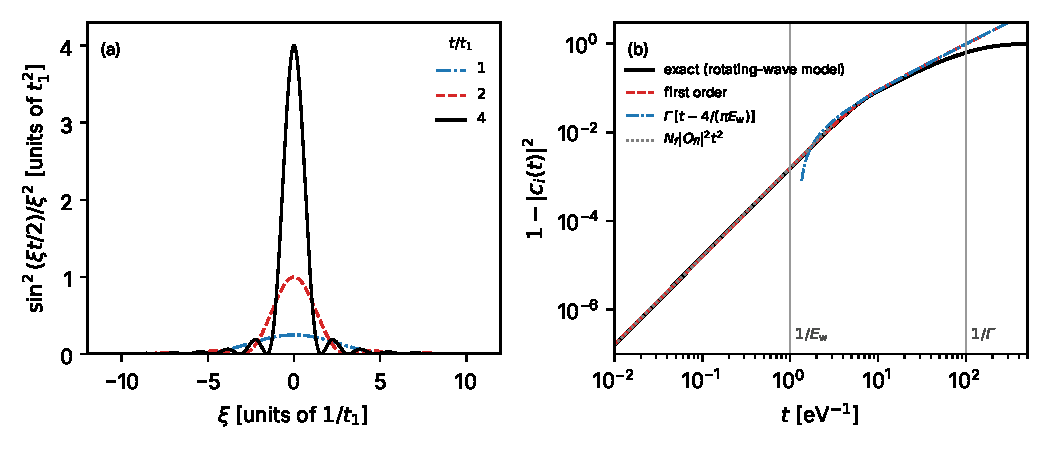
\includegraphics[width=\linewidth]{figures/ch02/fig2_1.pdf}
  \caption{(a) The function $\sin^2(\xi t/2)/\xi^2$ of the first-order transition probability, \cref{eq:2.1-Pstatic}, against the energy mismatch $\xi = E_f - E_i$, for times $t = t_1$, $2t_1$ and $4t_1$, where $t_1$ is an arbitrary unit of time ($\hbar = 1$). The peak height grows as $t^2$, the width as $1/t$, and the area, $\pi t/2$, as $t$. (b) Depletion $1 - |c_i(t)|^2$ of a discrete state coupled to a flat continuum by the absorption term of a harmonic perturbation, for the model of \cref{we:2-continuum}. It has 2000 final states spread uniformly over a width $E_{\mathrm{w}} = \SI{1}{eV}$ centered on resonance, all with the same matrix element, chosen so that the golden-rule rate is $\varGamma = \SI{10}{meV}$. Solid: exact solution of this model with the counter-rotating (emission) term dropped, by diagonalization of the 2001-level Hamiltonian in the frame rotating with the perturbation. Dashed: first-order probability, \cref{eq:2.1-WEP}. Dash-dotted: its linear long-time form. Dotted: its quadratic short-time form. Vertical lines mark $t = 1/E_{\mathrm{w}}$ (\SI{0.66}{fs}) and $t = 1/\varGamma$ (\SI{66}{fs}).}
  \label{fig:2-golden}
\end{figure}

\subsection{Conditions for a rate}

For a single discrete final state, however, \cref{eq:2.1-Pstatic} does not grow linearly. Off resonance it oscillates below $4|\langle f|H'|i\rangle|^2/\xi^2$; exactly on resonance it grows as $t^2$ until first order fails. A rate requires a continuum. Let $\mathcal{D}_f(E)\,\dd E$ be the number of final states with energies in $[E, E + \dd E]$, the \emph{density of final states}, and let $\overline{|\langle f|H'|i\rangle|^2}(E)$ be the average of the squared matrix element over those states. The total transition probability is then
\begin{equation*}
  \sum_f P_{i\to f}(t) = \int\dd E\,\mathcal{D}_f(E)\;\overline{|\langle f|H'|i\rangle|^2}(E)\;\frac{4\sin^2[(E - E_i)t/2]}{(E - E_i)^2} .
\end{equation*}
By \cref{eq:2.1-deltalimit} it becomes $\varGamma_i t$, with the total rate
\begin{equation}
  \varGamma_i = 2\pi\,\overline{|\langle f|H'|i\rangle|^2}(E_i)\;\mathcal{D}_f(E_i) .
  \label{eq:2.1-total}
\end{equation}
The catch is that $t$ has to sit in a window. Let $E_{\mathrm{w}}$ be the energy scale over which the product $\mathcal{D}_f\,\overline{|\langle f|H'|i\rangle|^2}$ changes appreciably: the width of the continuum, or of a structure within it. The delta-function limit needs the peak to be narrow on that scale, $t \gg 1/E_{\mathrm{w}}$. The sum over discrete levels becomes an integral only when the peak covers many levels, whose spacing is $1/\mathcal{D}_f$; this requires $t \ll 2\pi\mathcal{D}_f$. First-order perturbation theory requires $\varGamma_i t \ll 1$. Together,
\begin{equation}
  \frac{1}{E_{\mathrm{w}}} \ll t \ll \min\!\left(\frac{1}{\varGamma_i},\; 2\pi\mathcal{D}_f\right).
  \label{eq:2.1-window}
\end{equation}
In dark-matter scattering, however, the continuum is always present, even when the target has discrete levels, such as an atom below its ionization threshold. The final state contains the scattered dark-matter particle, whose momentum ranges over a continuum, and $\mathcal{D}_f$ counts target levels and dark-matter momenta together. Energy conservation then selects, for each target level, a shell of outgoing momenta, and the delta function of \cref{eq:2.1-golden} is integrated over that shell rather than over the target spectrum (\cref{sec:2.2}).

The upper bound $2\pi\mathcal{D}_f$ grows with the volume of the system, because $\mathcal{D}_f$ does (\cref{eq:2.1-Dfree}); it drops out when the infinite-volume limit is taken before the long-time limit, as we do throughout. The window then exists whenever $\varGamma_i \ll E_{\mathrm{w}}$: the transition must be slow compared with the inverse energy scale of the continuum.

At times beyond $1/\varGamma_i$ the initial state is depleted. The exact evolution then becomes exponential decay at the same rate $\varGamma_i$ (Wigner--Weisskopf; \cref{sec:2.4}), and $\varGamma_i$ keeps its meaning beyond the first-order window. For a dark-matter particle crossing a detector the condition $\varGamma_i t \ll 1$ holds by a wide margin, because the probability that it scatters at all during its passage is the small number that makes the searches of \cref{sec:1.5} difficult.

The golden rule also fails when the first-order matrix element vanishes and when the perturbation shifts the energy of the initial state. If $\langle f|H'|i\rangle$ vanishes for every final state at energy $E_i$, by a selection rule or because no such state exists, \cref{eq:2.1-total} vanishes, and the leading rate comes from the second-order amplitude through intermediate states (\cref{sec:2.4}). If the perturbation shifts the energy of $|i\rangle$ itself, by $\langle i|H'|i\rangle \neq 0$, the delta function must be evaluated at the shifted energy; the shift is of first order, while the rate is of second order in $H'$. For dark-matter scattering the diagonal element is the $\vect{q} = 0$ term of \cref{eq:2.1-Vbox}, $\tilde V(\vect{0})/\Vol$, which for a massive mediator vanishes as the volume grows, and the shift plays no role. For a massless mediator $\tilde V(\vect{0})$ itself diverges; in a neutral target the charges cancel this term, as \cref{sec:2.3} shows for the Coulomb interaction.

\subsection{Harmonic perturbations}

An absorbed bosonic dark-matter field oscillates in time at its mass (\cref{sec:1.4}), and an applied field oscillates at its frequency. Such a perturbation is harmonic,
\begin{equation*}
  H'(t) = \op{O}\,\ee^{-\ii\omega t} + \op{O}^\dagger\,\ee^{\ii\omega t}, \qquad \omega > 0,
\end{equation*}
where $\op{O}$ is an operator on the target and the second term makes $H'$ Hermitian. \Cref{eq:2.1-c1} now has two terms of the static form, with $\xi$ shifted by $\mp\omega$:
\begin{equation*}
  c_f(t) = -\langle f|\op{O}|i\rangle\,\frac{\ee^{\ii(\xi - \omega)t} - 1}{\xi - \omega} - \langle f|\op{O}^\dagger|i\rangle\,\frac{\ee^{\ii(\xi + \omega)t} - 1}{\xi + \omega} .
\end{equation*}
The first term peaks at $\xi = \omega$, the second at $\xi = -\omega$, each with width of order $2\pi/t$. For $\omega t \gg 1$ the peaks do not overlap. The cross term in $|c_f|^2$ is then bounded in time instead of growing, and each squared term turns into a delta function by \cref{eq:2.1-deltalimit}:
\begin{equation}
  \varGamma_{i\to f} = 2\pi\,|\langle f|\op{O}|i\rangle|^2\,\delta(E_f - E_i - \omega) + 2\pi\,|\langle f|\op{O}^\dagger|i\rangle|^2\,\delta(E_f - E_i + \omega) .
  \label{eq:2.1-harmonic}
\end{equation}
The first term is absorption: the target gains the energy $\omega$. The second is emission: the target gives $\omega$ to the field, so the energy given to the target is $-\omega$. With the temporal Fourier convention of \cref{app:A.3}, $f(\omega) = \int\dd t\,\ee^{+\ii\omega t}f(t)$, the factor $\ee^{-\ii\omega t}$ is the component of $H'$ at positive frequency, and positive frequency means energy given to the target. Since $|\langle f|\op{O}^\dagger|i\rangle| = |\langle i|\op{O}|f\rangle|$, emission from $i$ to $f$ and absorption from $f$ to $i$ have the same matrix element; \cref{sec:2.5} combines this with thermal populations into detailed balance.

For a classical field the emission term is stimulated emission, driven by the field itself. When the field is a quantized mode, the dark-matter or phonon state is part of $|i\rangle$ and $|f\rangle$, the perturbation is static, and \cref{eq:2.1-golden} applies to the combined system. Absorption removes a quantum and emission adds one, with matrix elements proportional to $\sqrt{n}$ and $\sqrt{n + 1}$ for a mode holding $n$ quanta (\cref{sec:2.3,sec:2.5}). The extra $1$ is spontaneous emission, which a classical field misses. At $\omega = 0$ the two peaks coincide, the cross term no longer averages out, and \cref{eq:2.1-harmonic} reduces to \cref{eq:2.1-golden} with $H' = \op{O} + \op{O}^\dagger$.

The harmonic form explains why the absorption rates of \cref{sec:1.4} depend on the local density of dark matter and not on its flux. A bosonic field of mass $m_\phi$ that makes up the local dark matter oscillates as $\phi(t) = \phi_0\cos(m_\phi t)$, with energy density $\tfrac12\dot\phi^2 + \tfrac12 m_\phi^2\phi^2 = \tfrac12 m_\phi^2\phi_0^2 = \rho_\chi$. Its spatial phase $\ee^{\ii\vect{p}_\phi\cdot\vect{x}}$ changes over a length $1/|\vect{p}_\phi| \approx 1/(m_\phi v)$, a thousand times the Compton wavelength $1/m_\phi$, and we neglect it here. An interaction linear in the field, $H' = \phi(t)$ times a target operator, is harmonic with $\omega = m_\phi$, and $\op{O}$ is $\phi_0/2$ times that operator. The absorption term of \cref{eq:2.1-harmonic} is therefore proportional to $\phi_0^2 = 2\rho_\chi/m_\phi^2$: the rate is fixed by the energy density of the field, and the speed of the dark matter does not enter. \Cref{chap:8} evaluates the target operators for each boson.

\begin{workedexample}{A harmonic perturbation coupled to a flat continuum}\label{we:2-continuum}
A discrete state $|i\rangle$ is coupled by the absorption term $\op{O}\,\ee^{-\ii\omega t}$ to $N_f$ final states spread uniformly over an energy width $E_{\mathrm{w}}$ centered on the resonance $E_f = E_i + \omega$. The density of final states is $\mathcal{D}_f = N_f/E_{\mathrm{w}}$, and every final state has the same $|\langle f|\op{O}|i\rangle|^2 \equiv |O_{fi}|^2$. With $\xi_f = E_f - E_i - \omega$, \cref{eq:2.1-Pstatic} with $H' \to \op{O}$ and $\xi \to \xi_f$, summed over $f$, gives the first-order depletion. For $t \ll 2\pi\mathcal{D}_f$ the sum is an integral, and the substitution $u = \xi t/2$ gives
\begin{equation*}
  P(t) = 4|O_{fi}|^2\mathcal{D}_f\int_{-E_{\mathrm{w}}/2}^{E_{\mathrm{w}}/2}\dd\xi\,\frac{\sin^2(\xi t/2)}{\xi^2}
  = 4|O_{fi}|^2\mathcal{D}_f\,t\int_0^{E_{\mathrm{w}}t/4}\dd u\,\frac{\sin^2u}{u^2} .
\end{equation*}
Integration by parts, with $\dd(-\sin^2u/u)/\dd u = \sin^2u/u^2 - \sin 2u/u$, gives $\int_0^U\dd u\,\sin^2u/u^2 = \operatorname{Si}(2U) - \sin^2U/U$, where $\operatorname{Si}(z) = \int_0^z\dd s\,\sin s/s$ is the sine integral. Hence
\begin{equation}
  P(t) = 4|O_{fi}|^2\mathcal{D}_f\,t\left[\operatorname{Si}\!\left(\frac{E_{\mathrm{w}}t}{2}\right) - \frac{\sin^2(E_{\mathrm{w}}t/4)}{E_{\mathrm{w}}t/4}\right].
  \label{eq:2.1-WEP}
\end{equation}
At short times, $E_{\mathrm{w}}t \ll 1$, the expansions $\operatorname{Si}(z) = z - z^3/18 + \dots$ and $\sin^2U/U = U - U^3/3 + \dots$ make the bracket $E_{\mathrm{w}}t/4$, so $P(t) = N_f|O_{fi}|^2t^2$. Every final state is populated, as if each were resonant: the energy is not yet resolved. At long times, $E_{\mathrm{w}}t \gg 1$, the asymptotic form $\operatorname{Si}(z) = \pi/2 - \cos z/z + O(z^{-2})$ and the identity $2\cos 2U + 4\sin^2U = 2$ make the bracket $\pi/2 - 2/(E_{\mathrm{w}}t)$, so
\begin{equation*}
  P(t) = \varGamma\left(t - \frac{4}{\pi E_{\mathrm{w}}}\right), \qquad \varGamma = 2\pi|O_{fi}|^2\mathcal{D}_f ,
\end{equation*}
up to terms that decay as $1/t$. We see that the probability grows linearly at the golden-rule rate \cref{eq:2.1-total}, delayed by $4/(\pi E_{\mathrm{w}})$, the time the system needs to resolve the energy.

For numbers we take $E_{\mathrm{w}} = \SI{1}{eV}$, $N_f = 2000$ (level spacing \SI{0.5}{meV}, $\mathcal{D}_f = \SI{2000}{eV^{-1}}$) and $|O_{fi}| = \SI{0.892}{meV}$, for which $\varGamma = \SI{10}{meV}$. With $\hbar = \SI{6.582e-16}{eV.s}$, the time scales are $1/E_{\mathrm{w}} = \SI{0.66}{fs}$, the delay $4/(\pi E_{\mathrm{w}}) = \SI{0.84}{fs}$, $1/\varGamma = \SI{66}{fs}$ and $2\pi\mathcal{D}_f = \SI{8.3}{ps}$, so the window \cref{eq:2.1-window} spans two orders of magnitude, from \SI{0.66}{fs} to \SI{66}{fs}. \Cref{fig:2-golden}(b) compares \cref{eq:2.1-WEP} with the exact evolution of the same model, obtained by solving \cref{eq:2.1-exact} with the emission term dropped. The substitution $\tilde c_f = c_f\,\ee^{\ii\xi_ft}$ (and $\tilde c_i = c_i$) removes every time-dependent phase from \cref{eq:2.1-exact}, since the absorption term carries $\ee^{-\ii\omega t}\ee^{\ii(E_f - E_i)t} = \ee^{\ii\xi_ft}$; in this frame, which rotates with the perturbation, the coefficients are constant and the model is a time-independent Hamiltonian of 2001 levels, which we diagonalize numerically. First order exceeds the exact depletion by \SI{10}{\percent} at $t = \SI{21.9}{eV^{-1}}$, where $\varGamma t = 0.22$; at $t = 1/\varGamma$ it predicts $0.99$ against the exact $0.63$. First order therefore breaks down at $\varGamma t \approx 0.2$. Beyond it the exact depletion follows $1 - \ee^{-\varGamma t}$, within \SI{0.4}{\percent} from $t = 1/\varGamma$ on, which is the exponential decay of \cref{sec:2.4} with the golden-rule rate as its decay constant.
\end{workedexample}

\subsection{Box normalization and final-state sums}

With plane waves normalized in infinite volume, $\langle\vect{p}|\vect{p}'\rangle = (2\pi)^3\delta^3(\vect{p} - \vect{p}')$, momentum conservation in a matrix element is a delta function, and \cref{eq:2.1-golden} squares it. The square $[\delta^3(\vect{P}_f - \vect{P}_i)]^2$ has no meaning on its own. A finite box makes every step well defined: momenta are discrete, momentum conservation is a Kronecker delta, whose square is itself, and the golden rule needs countable states to sum over. We therefore place the system in a cube of volume $\Vol = L^3$ with periodic boundary conditions. The plane waves $\langle\vect{x}|\vect{p}\rangle = \ee^{\ii\vect{p}\cdot\vect{x}}/\sqrt{\Vol}$, with $\vect{p} = 2\pi\vect{n}/L$ and $\vect{n}$ a vector of integers, obey $\langle\vect{p}|\vect{p}'\rangle = \delta_{\vect{p}\vect{p}'}$: each state holds one particle in the volume $\Vol$. The script $\Vol$ always denotes this volume; an italic $V$ is a potential and always carries its argument, $V(\vect{x})$, or a tilde, $\tilde V(\vect{q})$. Since each allowed momentum occupies a cell of volume $(2\pi)^3/\Vol$, for any function that varies little over $2\pi/L$~\cite[Eqs.~(A1) and (A2)]{lin2019tasi}
\begin{equation}
  \sum_{\vect{p}}w(\vect{p}) \;\to\; \Vol\int\frac{\dd^3p}{(2\pi)^3}\,w(\vect{p}), \qquad
  \delta_{\vect{p}\vect{p}'} \;\to\; \frac{(2\pi)^3}{\Vol}\,\delta^3(\vect{p} - \vect{p}') .
  \label{eq:2.1-box}
\end{equation}
\Cref{app:A.3} collects these conventions and \cref{app:C.2} the continuum limit of such sums, including sums over the Brillouin zone. For one free particle of mass $m$ with energy $E = p^2/2m$, the number of states in a shell is $\Vol\,4\pi p^2\,\dd p/(2\pi)^3$, and with $\dd E = p\,\dd p/m$ we find
\begin{equation}
  \mathcal{D}_f(E) = \frac{\Vol\,m\,p}{2\pi^2}, \qquad p = (2mE)^{1/2} .
  \label{eq:2.1-Dfree}
\end{equation}
The density of final states is proportional to $\Vol$. In a crystal the box is a block of $N$ unit cells, and the same counting applies to crystal momenta (\cref{sec:3.1}). Discrete quantum numbers, such as spin, are summed separately in the final state. When the initial state is not known exactly, the rate is averaged over it: over the two spin states of an unpolarized particle, and over a thermal ensemble of target states (\cref{sec:2.5}).

The volume must drop out of every observable, and in a finite box we can follow it through every rate as a check. Consider a dark-matter particle and an electron, both box-normalized, interacting through a potential $V(\vect{x}_\chi - \vect{x}_e)$ of their separation (\cref{sec:1.4}). Writing $\vect{r} = \vect{x}_\chi - \vect{x}_e$ and integrating over $\vect{x}_e$ at fixed $\vect{r}$,
\begin{equation}
  \langle\vect{p}_\chi',\vect{p}_e'|V(\vect{x}_\chi - \vect{x}_e)|\vect{p}_\chi,\vect{p}_e\rangle
  = \frac{1}{\Vol^2}\int\dd^3x_e\,\ee^{-\ii(\vect{P}_f - \vect{P}_i)\cdot\vect{x}_e}\int\dd^3r\,\ee^{\ii\vect{q}\cdot\vect{r}}\,V(\vect{r})
  = \frac{\tilde V(\vect{q})}{\Vol}\,\delta_{\vect{P}_f\vect{P}_i} ,
  \label{eq:2.1-Vbox}
\end{equation}
with $\vect{q} = \vect{p}_\chi - \vect{p}_\chi'$ the momentum transferred to the electron, $\vect{P}_{i,f}$ the initial and final total momenta, and $\tilde V(\vect{q})$ the transform of \cref{app:A.3}. Each plane wave brings $\Vol^{-1/2}$ and the integral over the position of the pair brings $\Vol$ times momentum conservation. In \cref{eq:2.1-golden} the squared matrix element brings $1/\Vol^2$, and the sum over one final momentum, the other being fixed by $\delta_{\vect{P}_f\vect{P}_i}$, brings $\Vol$. We see that the rate is proportional to $1/\Vol$: it is the rate at which two particles placed in the same box find each other.

A cross-section removes this factor. Since the incident particle has density $1/\Vol$ and speed $v$ relative to the target, its flux is $v/\Vol$ (\cref{eq:1.2-flux}, with a single velocity), and the rate per target particle is that flux times the cross-section $\sigma_T$ for scattering on one target particle. Hence
\begin{equation}
  \sigma_T = \frac{\Vol}{v}\,\varGamma = \frac{\Vol}{v}\sum_f 2\pi\,|\langle f|H'|i\rangle|^2\,\delta(E_f - E_i),
  \label{eq:2.1-sigma}
\end{equation}
which is independent of $\Vol$. The rate in a detector follows by reversing the argument. Dark matter with velocity in $\dd^3v$ crosses a target particle with flux $\nd_\chi f_\chi(\vect{v})\,\dd^3v\,v$ (\cref{sec:1.2}). Integrating over velocities and multiplying by the number of target particles per unit mass, $1/m_T$ with $m_T$ the mass of one, leads to an event rate per unit mass $(\rho_\chi/m_\chi m_T)\int\dd^3v\,f_\chi(\vect{v})\,v\,\sigma_T(v)$, the structure that \cref{sec:1.5} assembled for a target with a response.

For readers comparing with particle-physics papers, we also translate to relativistic normalization, $\langle\vect{p}|\vect{p}'\rangle_{\mathrm{rel}} = 2E_{\vect{p}}(2\pi)^3\delta^3(\vect{p} - \vect{p}')$~\cite[Chap.~2]{peskin1995introduction}; it is used again only to compare with the literature (\cref{sec:2.4,app:A.9}). In the box, $(2\pi)^3\delta^3(\vect{0}) \to \Vol$ by \cref{eq:2.1-box}, and $\langle\vect{p}|\vect{p}\rangle_{\mathrm{rel}} = 2E_{\vect{p}}\Vol$: the state holds $2E_{\vect{p}}$ particles per unit volume, and $|\vect{p}\rangle_{\mathrm{rel}} = (2E_{\vect{p}}\Vol)^{1/2}|\vect{p}\rangle$. At first order the invariant amplitude $\mathcal{M}$ of a process $1 + 2 \to 3 + 4$ is defined by $\langle f|H'|i\rangle_{\mathrm{rel}} = -\mathcal{M}\,(2\pi)^3\delta^3(\vect{P}_f - \vect{P}_i)$, the first-order term of $\langle f|\ii\op{T}|i\rangle = \ii(2\pi)^4\delta^4(P_f - P_i)\,\mathcal{M}$ once the time integral has produced $2\pi\delta(E_f - E_i)$~\cite[Chap.~4]{peskin1995introduction}. Dividing by the four normalization factors and using $(2\pi)^3\delta^3 \to \Vol\delta_{\vect{P}_f\vect{P}_i}$ gives the box matrix element $\langle f|H'|i\rangle = -\mathcal{M}\,\delta_{\vect{P}_f\vect{P}_i}/[\Vol\prod_{j=1}^4(2E_j)^{1/2}]$. Inserted into \cref{eq:2.1-sigma}, with the sum over $\vect{p}_3$ turned into an integral,
\begin{equation*}
  \sigma_T = \frac{1}{2E_1\,2E_2\,v}\int\frac{\dd^3p_3}{(2\pi)^3\,2E_3}\,\frac{2\pi}{2E_4}\,|\mathcal{M}|^2\,\delta(E_f - E_i),
\end{equation*}
the relativistic formula with its flux factor and two-body phase space~\cite[Chap.~4]{peskin1995introduction}. The factors $2E$ that the relativistic normalization puts into the states reappear as $1/2E$ in the flux and the phase space. We use box normalization throughout, because a crystal is not Lorentz invariant and its states are naturally normalized to one per crystal volume. In the nonrelativistic limit $2E_j \to 2m_j$, and for elastic dark-matter--electron scattering comparison with \cref{eq:2.1-Vbox} leads to $|\mathcal{M}|^2 = 16m_\chi^2m_e^2|\tilde V(\vect{q})|^2$. The definition of $\sigmae$ in \cref{eq:1.4-defs} then takes the form $\mu_{\chi e}^2|\mathcal{M}(q_0)|^2/(16\pi m_\chi^2m_e^2)$ used in the particle-physics literature~\cite[Eq.~(3)]{essig2012direct}.

\section{Born approximation and form factors}\label{sec:2.2}

A dark-matter particle of \SI{100}{MeV} that meets a free electron scatters with the cross-section $\mu_{\chi e}^2|\tilde V|^2/\pi$ when the mediator is heavy. \Cref{sec:1.4} defined $\sigmae$ through this cross-section. The same golden-rule calculation yields the rate off an electron bound in an atom, where the electron's wavefunction enters through a single overlap, the transition form factor, and the rate off a nucleus, whose nucleons scatter in phase and multiply the cross-section by $A^2$. We derive all three from \cref{eq:2.1-golden,eq:2.1-Vbox}, to first order in the potential: the first Born approximation.

\subsection{The Born cross-section}

Take a dark-matter particle and an electron in a box, interacting through a potential $V(\vect{x}_\chi - \vect{x}_e)$ of their separation. Since the total momentum is conserved, it is simplest to work in the center-of-mass frame, where the dark matter has momentum $\vect{p}$, the electron $-\vect{p}$, and the relative speed is $v = p/\mu_{\chi e}$. The kinetic energy of relative motion is $p^2/2\mu_{\chi e}$. In general the Hamiltonian splits as $P_{\mathrm{tot}}^2/2(m_\chi + m_e) + p_{\mathrm{rel}}^2/2\mu_{\chi e} + V(\vect{r})$, with $\vect{P}_{\mathrm{tot}}$ the total momentum, $\vect{p}_{\mathrm{rel}}$ the relative momentum and $\vect{r}$ the separation. The potential acts on the relative motion alone, which is a single particle of mass $\mu_{\chi e}$; the center of mass moves freely and drops out of the cross-section. A transition to $\vect{p}' = \vect{p} - \vect{q}$ has the box matrix element $\tilde V(\vect{q})/\Vol$ of \cref{eq:2.1-Vbox}, with $\vect{q}$ the momentum transferred to the electron. The potential does not act on spin, and the spins need no sum. Inserting this into the cross-section of \cref{eq:2.1-sigma} and summing over the one free final momentum,
\begin{equation*}
  \sigma_T = \frac{\Vol}{v}\sum_{\vect{p}'}2\pi\,\frac{|\tilde V(\vect{q})|^2}{\Vol^2}\,\delta\!\left(\frac{p'^2}{2\mu_{\chi e}} - \frac{p^2}{2\mu_{\chi e}}\right)
  = \frac{1}{v}\int\frac{p'^2\,\dd p'\,\dd\Omega_{\vect{q}}}{(2\pi)^3}\;2\pi\,|\tilde V(\vect{q})|^2\,\frac{\mu_{\chi e}}{p}\,\delta(p' - p),
\end{equation*}
where we used \cref{eq:2.1-box} for the sum and $\delta(p'^2/2\mu_{\chi e} - p^2/2\mu_{\chi e}) = (\mu_{\chi e}/p)\,\delta(p' - p)$, the rule $\delta(g(x)) = \delta(x - x_0)/|g'(x_0)|$ for a simple root $x_0$ (\cref{app:C.1}). Here $\dd\Omega_{\vect{q}}$ is the element of solid angle of the scattered momentum $\vect{p}'$ (the literature writes $\dd\Omega$). The volume has dropped out, as it must. Doing the radial integral and using $p = \mu_{\chi e}v$,
\begin{keyresult}[Born cross-section]
\begin{equation}
  \frac{\dd\sigma_T}{\dd\Omega_{\vect{q}}} = \left(\frac{\mu_{\chi e}}{2\pi}\right)^2|\tilde V(\vect{q})|^2 ,
  \qquad |\vect{q}| = 2p\sin(\theta_{\mathrm{s}}/2),
  \label{eq:2.2-born}
\end{equation}
with $\theta_{\mathrm{s}}$ the scattering angle between $\vect{p}$ and $\vect{p}'$. For dark-matter--nucleus scattering $\mu_{\chi e}$ becomes $\mu_{\chi N}$.
\end{keyresult}
This is the textbook first Born approximation~\cite[Chap.~6]{sakurai2017modern}: the scattering amplitude is $-(\mu_{\chi e}/2\pi)\tilde V(\vect{q})$, and its square is the differential cross-section. The minus sign makes the amplitude positive for an attractive potential, and it drops out of every rate. The momentum transfer $\vect{q} = \vect{p} - \vect{p}'$ is the same in the laboratory frame, because a Galilean boost shifts $\vect{p}$ and $\vect{p}'$ by the same amount (\cref{sec:1.2}).

A quick check is Coulomb scattering. For $m_V \to 0$ and couplings $y_\chi y_e \to e^2 = 4\pi\alpha$, \cref{eq:1.4-Vq} becomes $\tilde V = 4\pi\alpha/q^2$, and \cref{eq:2.2-born} becomes $\dd\sigma_T/\dd\Omega_{\vect{q}} = 4\mu_{\chi e}^2\alpha^2/q^4 = \alpha^2/[4\mu_{\chi e}^2v^4\sin^4(\theta_{\mathrm{s}}/2)]$, Rutherford's formula. Its divergence at small angle, $\theta_{\mathrm{s}}^{-4}$, is the divergence of $\sigmae$ for a light mediator noted in \cref{sec:1.4}.

The approximation keeps one power of $V(\vect{x})$ in the amplitude. The next term, of second order (\cref{sec:2.4}), is small when the potential barely distorts the incoming wave over its range. For a Yukawa potential of range $1/m_V$ and strength $y_\chi y_e$ (\cref{eq:1.4-yukawa}) this needs, up to $O(1)$ factors, $y_\chi y_e\,\mu_{\chi e}/(4\pi m_V) \ll 1$ at low energy and $y_\chi y_e/(4\pi v) \ll 1$ when the de Broglie wavelength is shorter than the range~\cite[Chap.~6]{sakurai2017modern}. The second condition is the familiar $\alpha/v \ll 1$ of Coulomb scattering. For the heavy dark photon of \cref{we:1-darkphoton}, $y_\chi y_e = y_\chi\zeta e = 9\times10^{-6}$, and both parameters are below $10^{-3}$ at $v = 10^{-3}$. Couplings of dark matter to ordinary matter are always this weak, because larger ones are excluded (\cref{sec:1.4}), and first order is sufficient for our purposes. The exception is the dark sector itself, where self-interactions can be strong; it does not enter a detector. Screening in a target is not a higher Born term either. It comes from the target's electrons rearranging in response to the potential, at first order in $V(\vect{x})$ but to all orders in the Coulomb interaction among themselves, and it belongs to the target response (\cref{sec:4.4}).

The rate needs the distribution in $q$ rather than in angle. From $q^2 = 2p^2(1 - \cos\theta_{\mathrm{s}})$, the solid angle is $\dd\Omega_{\vect{q}} = 2\pi\,\dd\cos\theta_{\mathrm{s}} = \pi\,\dd q^2/p^2 = 2\pi q\,\dd q/(\mu_{\chi e}^2v^2)$ after the trivial azimuthal integral. \Cref{eq:2.2-born} then gives
\begin{equation}
  \frac{\dd\sigma_T}{\dd q} = \frac{q\,|\tilde V(\vect{q})|^2}{2\pi v^2}
  = \frac{q\,\sigmae}{2\mu_{\chi e}^2v^2}\,\FDM(q)^2 , \qquad 0 \le q \le 2\mu_{\chi e}v ,
  \label{eq:2.2-dsdq}
\end{equation}
where the form in $\sigmae$ uses $|\tilde V|^2 = \pi\sigmae\FDM^2/\mu_{\chi e}^2$ (\cref{eq:1.4-Vsq}). The upper limit is backscattering, $\theta_{\mathrm{s}} = \pi$. For a contact interaction, $\FDM = 1$, the distribution rises linearly in $q$ and integrates to
\begin{equation}
  \sigma_T = \frac{|\tilde V|^2}{2\pi v^2}\,\frac{(2\mu_{\chi e}v)^2}{2} = \frac{\mu_{\chi e}^2|\tilde V|^2}{\pi} = \sigmae ,
  \label{eq:2.2-sigma-free}
\end{equation}
independent of the speed. This is the statement behind the definition of $\sigmae$ in \cref{eq:1.4-defs}: for a heavy mediator, $\sigmae$ is the total cross-section of dark matter on a free electron (also \cref{eq:A.9-dsdq}). For a nucleus, $\mu_{\chi e} \to \mu_{\chi N}$ and $\sigmae \to \sigma_N$; we return to it at the end of the section.

\subsection{Scattering off a bound electron}

An electron bound in an atom or a crystal does not conserve momentum by itself. The nucleus, or the lattice, absorbs whatever momentum the electron does not keep, and the electron jumps between states $|i\rangle$ and $|f\rangle$ of its own Hamiltonian instead of between plane waves. We treat the binding potential as fixed in space, which neglects the recoil of a nucleus thousands of times heavier than the electron. The dark matter is still a plane wave. The matrix element follows from the same step as \cref{eq:2.1-Vbox}: integrating over the dark-matter position at fixed electron position $\vect{r}$ (\cref{eq:A.3-vertex}) gives
\begin{equation}
  \langle\vect{p} - \vect{q}, f|V(\vect{x}_\chi - \vect{r})|\vect{p}, i\rangle = \frac{\tilde V(\vect{q})}{\Vol}\,f_{i\to f}(\vect{q}),
  \qquad
  f_{i\to f}(\vect{q}) \equiv \langle f|\ee^{\ii\vect{q}\cdot\vect{r}}|i\rangle = \int\dd^3r\;\psi_f^*(\vect{r})\,\ee^{\ii\vect{q}\cdot\vect{r}}\,\psi_i(\vect{r}) .
  \label{eq:2.2-ff}
\end{equation}
The \emph{transition form factor} $f_{i\to f}(\vect{q})$ is the amplitude for the electron to absorb the momentum $\vect{q}$ and end up in $|f\rangle$. It is a property of the target alone; the dark matter enters only through $\tilde V(\vect{q})$. Its sign convention follows that of $\tilde V$ (\cref{app:A.3}). For free electrons, $\psi_i$ and $\psi_f$ are plane waves and $f_{i\to f}$ is a Kronecker delta that conserves momentum, so \cref{eq:2.1-Vbox} is the special case.

The energy that the dark matter loses, $p^2/2m_\chi - (\vect{p} - \vect{q})^2/2m_\chi = \vect{q}\cdot\vect{v} - q^2/2m_\chi$, is the energy deposit $\omega_{\vect{q}}$ of \cref{eq:1.3-omegaq} (with $\Delta_\chi = 0$; an inelastic dark-matter particle adds $-\Delta_\chi$). The golden rule, summed over the final dark-matter momentum by \cref{eq:2.1-box} and over the final electron state, yields the rate $\varGamma$ per dark-matter particle in the box. The box holds one dark-matter particle, a density $1/\Vol$. The volume-independent combination is $\Vol\varGamma$, which is $\sigma_T v$ by \cref{eq:2.1-sigma}:
\begin{keyresult}[Rate off a bound target]
\begin{equation}
  \sigma_T v = \Vol\varGamma = \int\frac{\dd^3q}{(2\pi)^3}\,|\tilde V(\vect{q})|^2\sum_f|f_{i\to f}(\vect{q})|^2\;2\pi\,\delta(E_f - E_i - \omega_{\vect{q}}) .
  \label{eq:2.2-bound}
\end{equation}
The target enters only through $|f_{i\to f}(\vect{q})|^2$ and the excitation energies $E_f - E_i$; the dark matter only through $|\tilde V(\vect{q})|^2$ and $\omega_{\vect{q}}$.
\end{keyresult}
\noindent With $|\tilde V|^2$ written through \cref{eq:1.4-Vsq}, \cref{eq:2.2-bound} becomes $\sigma_T v = (\sigmae/\mu_{\chi e}^2)\int\dd^3q\,(4\pi)^{-1}\FDM^2\sum_f|f_{i\to f}|^2\,\delta(E_f - E_i - \omega_{\vect{q}})$~\cite[Eqs.~(3.9) and (3.10)]{essig2016direct}.

Depositing an energy $\omega$ needs $q \ge \omega/v$, since $\omega_{\vect{q}} \le qv$, and this decides which momentum transfers \cref{eq:2.2-bound} weights. A bound electron absorbs momentum transfers up to about its own momentum, $q_0 = \alpha m_e$ for an outer electron, and beyond that $|f_{i\to f}|^2$ collapses. The two requirements meet at $\omega \approx q_0v \approx \alpha m_ev \approx \SI{4}{eV}$ for $v \approx 10^{-3}$, independent of $m_\chi$ (\cref{sec:1.3}). This is why eV-gap targets are a good kinematic match to sub-GeV dark matter: the silicon gap of \SI{1.11}{eV} used in projections sits below this energy, and the momentum transfers that cross it, $q \gtrsim \SI{0.42}{keV}$ at $v_{\mathrm{max}}$ (\cref{sec:1.3}), are ones the valence electrons absorb readily. Ionizing hydrogen, $\omega \ge \SI{13.6}{eV}$, needs $q \ge \SI{5.1}{keV} = 1.4\,q_0$ even at the largest halo speed $v_{\mathrm{max}} = 2.65\times10^{-3}$, and a dark-matter mass of at least $2\times\SI{13.6}{eV}/v_{\mathrm{max}}^2 = \SI{3.9}{MeV}$ (\cref{eq:1.3-mmin}). The form factor at such $q$ is not yet small, as the hydrogen example shows, but the halo factor $\eta(\vmin)$ is, because only the fastest dark matter can supply the energy.

Closure fixes the total size of the form factor. Summed over a complete set of final states, bound and free, and including $|i\rangle$ itself,
\begin{equation}
  \sum_f|f_{i\to f}(\vect{q})|^2 = \langle i|\ee^{-\ii\vect{q}\cdot\vect{r}}\ee^{\ii\vect{q}\cdot\vect{r}}|i\rangle = 1 .
  \label{eq:2.2-closure}
\end{equation}
The electron absorbs the momentum $\vect{q}$ with total probability one; the form factor distributes that probability over final states. The term $f = i$ is the \emph{elastic form factor} $f_{i\to i}(\vect{q}) = \int\dd^3r\,|\psi_i(\vect{r})|^2\,\ee^{\ii\vect{q}\cdot\vect{r}}$, the Fourier transform of the electron's charge cloud. An electron bound in an orbital of radius $r$ has momenta $\sim 1/r$. A momentum transfer much smaller than $1/r$ barely changes the state, so the elastic term takes almost all of the probability, $f_{i\to i} \to 1$. A momentum transfer much larger than $1/r$ must be absorbed by the high-momentum tail of the wavefunction, and every overlap with a bound final state falls off. This is the physical picture behind $q_0 = \alpha m_e$ in \cref{sec:1.3}, and the hydrogen atom checks it below.

An atom with $Z$ electrons shows the same split on a larger scale. The target operator is now $\sum_{j=1}^Z\ee^{\ii\vect{q}\cdot\vect{r}_j}$, and its elastic matrix element in the atomic ground state is the transform of the total electron density, which tends to $Z$ as $q \to 0$. Elastic scattering at small $q$ is coherent, with a cross-section proportional to $Z^2$. Inelastic transitions, in which one electron changes its orbital, add incoherently, with total weight at most $Z$ by closure applied to each electron. The nucleus repeats this pattern with $A$ nucleons, at the end of the section. In a crystal the coherent part is the Bragg-like elastic response at reciprocal-lattice vectors, which deposits no energy, and the incoherent part is the electronic excitation a detector sees (\cref{chap:4}).

The rate in a detector averages \cref{eq:2.2-bound} over the dark-matter velocities. For a target whose $\sum_f|f_{i\to f}(\vect{q})|^2$ at fixed energy depends only on $q = |\vect{q}|$, such as an atom with closed shells, only the angle between $\vect{q}$ and $\vect{v}$ enters the delta function. Its average over that angle is $\Theta(v - \vmin)/(2qv)$, and the halo average turns $\Theta(v - \vmin)/v$ into $\eta(\vmin)$, the mean inverse speed of the dark matter above $\vmin$ (\cref{eq:1.3-eta}). Inserting $1 = \int\dd\omega\,\delta(\omega - E_f + E_i)$ and writing $\dd^3q = 4\pi q^2\,\dd q$ for the remaining integral,
\begin{equation}
  \frac{\dd\langle\sigma_T v\rangle}{\dd\omega} = \frac{1}{2\pi}\int q\,\dd q\;|\tilde V(q)|^2\,\eta\bigl(\vmin(q, \omega)\bigr)\sum_f|f_{i\to f}(q)|^2\,\delta(\omega - E_f + E_i) ,
  \label{eq:2.2-spectrum}
\end{equation}
with $\langle\cdot\rangle$ the average over the halo. A potential that does not act on spin leaves the spin of the electron unchanged, and each occupied orbital contributes once for each of its two spin states. A full shell of angular momentum $l$ therefore holds $2(2l + 1)$ electrons. Its density is spherical, because $\sum_m|Y_{lm}|^2 = (2l + 1)/4\pi$ for the spherical harmonics $Y_{lm}$ (\cref{app:C.3}), and so is its summed response to $\vect{q}$. A crystal is not spherical, and \cref{eq:2.2-bound} must then be kept with its angular integral; \cref{sec:1.2} gave the resulting daily modulation.

For a gas of such atoms with number density $\nd_T$, the event rate per unit target mass is $(\rho_\chi/m_\chi)(\nd_T/\rho_T)\langle\sigma_T v\rangle$. Comparing with \cref{eq:1.5-rate} identifies the target response of a gas of independent atoms: $S(q, \omega) = 2\pi\,\nd_T\sum_i\sum_f|f_{i\to f}(q)|^2\,\delta(\omega - E_f + E_i)$, summed over the occupied initial states $i$ of each atom. For any target, $S(q, \omega)$ is the dynamic structure factor of the density operator $n_e(\vect{q}) = \sum_j\ee^{\ii\vect{q}\cdot\vect{r}_j}$ of \cref{eq:A.3-ne} (\cref{eq:2.5-golden,eq:A.7-S}), whose single-electron matrix elements are the $f_{i\to f}$ of \cref{eq:2.2-ff}.

For several electrons the sum over $i$ runs over occupied states and the final states must be empty; second quantization (\cref{sec:2.3}) is the bookkeeping that handles this, and \cref{sec:4.2} recovers \cref{eq:2.2-spectrum} as the independent-particle limit. A target at finite temperature starts in a mixture of states $|i\rangle$, and the rate is averaged over them with thermal weights (\cref{sec:2.5}).

\subsection{The hydrogen atom}

The hydrogen ground state is the one bound electron whose form factor we can write in closed form. Its wavefunction is $\psi_{1s}(\vect{r}) = \ee^{-r/a_0}/(\pi a_0^3)^{1/2}$, with the Bohr radius $a_0 = 1/(\alpha m_e) = \SI{0.5292}{\angstrom}$ (\cref{app:A.1}). The reference momentum of \cref{sec:1.3} is its inverse, $q_0 = \alpha m_e = 1/a_0$, so $q_0a_0 = 1$ exactly.

\begin{workedexample}{The hydrogen 1s elastic form factor}\label{we:2-hydrogen}
The elastic form factor is the Fourier transform of $|\psi_{1s}|^2 = \ee^{-2r/a_0}/(\pi a_0^3)$. Since the density is spherical, the integral of $\ee^{\ii\vect{q}\cdot\vect{r}}$ over the directions of $\vect{r}$ gives $4\pi\sin(qr)/(qr)$ (\cref{app:C.3}), and
\begin{equation*}
  \begin{split}
  F_{1s}(q) \equiv f_{1s\to1s}(\vect{q}) &= \frac{4\pi}{\pi a_0^3}\int_0^\infty\dd r\,r^2\,\ee^{-2r/a_0}\,\frac{\sin qr}{qr}\\
  &= \frac{4}{a_0^3q}\int_0^\infty\dd r\,r\,\ee^{-\lambda_{1s}r}\sin qr , \qquad \lambda_{1s} = \frac{2}{a_0} .
  \end{split}
\end{equation*}
The remaining integral is the imaginary part of $\int_0^\infty\dd r\,r\,\ee^{-(\lambda_{1s} - \ii q)r} = 1/(\lambda_{1s} - \ii q)^2 = (\lambda_{1s} + \ii q)^2/(\lambda_{1s}^2 + q^2)^2$, which is $2\lambda_{1s}q/(\lambda_{1s}^2 + q^2)^2$. So $F_{1s}(q) = (4/a_0^3q)\,(4q/a_0)/(4/a_0^2 + q^2)^2$, or
\begin{equation}
  F_{1s}(q) = \frac{16}{(4 + q^2a_0^2)^2} .
  \label{eq:2.2-F1s}
\end{equation}
At small $q$, $F_{1s} = (1 + q^2a_0^2/4)^{-2} \simeq 1 - q^2a_0^2/2$. This is the general small-$q$ form $1 - q^2\langle r^2\rangle/6$ of an elastic form factor, with $\langle r^2\rangle = 3a_0^2$ for the 1s state. At large $q$, $F_{1s} \simeq 16/(qa_0)^4$: the elastic amplitude dies as the fourth power of the momentum transfer. The value at the reference momentum is $F_{1s}(q_0) = 16/25 = 0.64$: the electron stays in its ground state with probability $F_{1s}^2 = 0.41$ and, by \cref{eq:2.2-closure}, is excited or ionized with probability $0.59$. The form factor falls to one half at $qa_0 = 1.29$ and to $0.25$ at $qa_0 = 2$; its square falls to one half at $qa_0 = 0.87$. The 1s electron is the most compact state of hydrogen, and $q_0$ is close to the momentum transfer at which it stops responding as a whole and starts to be knocked out.

Where does the inelastic probability go? The lowest excitation, $1s \to 2p$ at \SI{10.2}{eV}, has a closed form too. Take $\vect{q}$ along $z$. Only the $m = 0$ state $\psi_{2p} = (32\pi a_0^5)^{-1/2}\,z\,\ee^{-r/2a_0}$ couples, because the operator $\ee^{\ii qz}$ does not change the angular momentum about $z$. The angular integral is $2\pi\int_{-1}^1\dd u\,u\,\ee^{\ii qru} = 4\pi\ii\,j_1(qr)$, with $j_1(x) = (\sin x - x\cos x)/x^2$ the spherical Bessel function of order one (\cref{app:C.3}), and the radial integral, done as in the elastic case with $\lambda_{2p} = 3/2a_0$, is $\int_0^\infty\dd r\,r^3\ee^{-\lambda_{2p}r}j_1(qr) = 8\lambda_{2p}q/(\lambda_{2p}^2 + q^2)^3$. Collecting the normalizations,
\begin{equation*}
  |f_{1s\to2p}(q)|^2 = \frac{72\,(qa_0)^2}{(9/4 + q^2a_0^2)^6} .
\end{equation*}
At small $q$ it grows as $(2^{15}/3^{10})\,q^2a_0^2 = 0.555\,q^2a_0^2$, which is $q^2|\langle 2p|z|1s\rangle|^2$: a momentum transfer much smaller than $1/a_0$ acts on the atom as a weak uniform field, through its dipole. The square peaks at $qa_0 = 0.67$ with the value $0.084$ and is $0.061$ at $q_0$. So at $q_0$ the $2p$ level takes about a tenth of the inelastic probability of $0.59$, and the rest goes to higher levels and, mostly, to ionization.
\end{workedexample}

\begin{figure}[tbp]
  \centering
  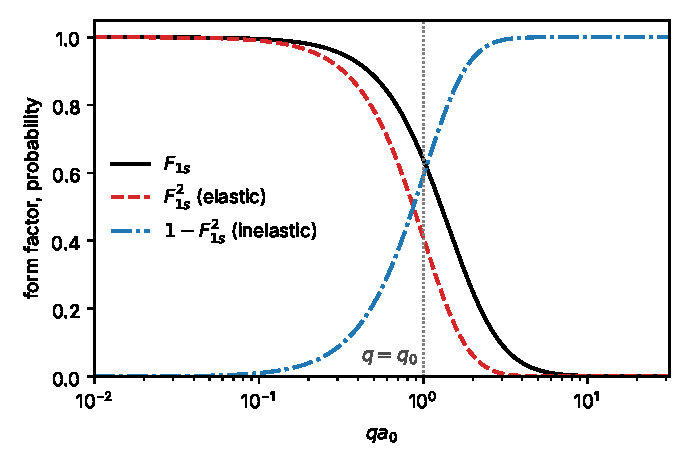
\includegraphics[width=0.62\linewidth]{figures/ch02/fig2_2.pdf}
  \caption{Hydrogen 1s elastic form factor $F_{1s}(q) = 16/(4 + q^2a_0^2)^2$ (solid), its square, the probability that the electron stays in the ground state after absorbing momentum $q$ (dashed), and the probability $1 - F_{1s}^2$ that it is excited or ionized (dash-dotted), against $qa_0$, with $a_0$ the Bohr radius. The dotted line marks the reference momentum $q_0 = \alpha m_e = \SI{3.73}{keV}$, where $qa_0 = 1$ exactly and $F_{1s} = 0.64$. The inelastic probability follows from the closure relation $\sum_f|\langle f|\ee^{\ii\vect{q}\cdot\vect{r}}|1s\rangle|^2 = 1$.}
  \label{fig:2-hydrogen}
\end{figure}

\Cref{fig:2-hydrogen} shows the crossover. Below $q \approx q_0/3$ the atom absorbs the momentum transfer elastically: the electron and the nucleus move together, and the energy deposit is the recoil of the whole atom. Above $q \approx 3q_0$ almost every scattering excites or ionizes the atom. The elastic form factor also explains how a neutral atom hides its charge. A dark photon couples to the electron and to the proton with opposite signs (\cref{sec:1.4}), and the elastic amplitude off the atom is proportional to $1 - F_{1s}(q)$: the proton, a point, contributes $1$, and the electron cloud $-F_{1s}$. At $q \ll q_0$ the two cancel and the dark matter sees a neutral atom; at $q_0$ the squared factor is $(1 - 0.64)^2 = 0.13$. This is screening in its simplest form, and \cref{sec:4.4} treats it in solids.

For ionization the final state is an unbound electron of momentum $p_{\mathrm{ej}}$ and kinetic energy $E_{\mathrm{ej}} = p_{\mathrm{ej}}^2/2m_e$, and the energy transfer is $\omega = E_B + E_{\mathrm{ej}}$, with $E_B > 0$ the binding energy of the shell. Far from the atom the ejected electron is a spherical wave; near it, the wave is distorted by the ion. The sum over final states in \cref{eq:2.2-spectrum} becomes an integral over $p_{\mathrm{ej}}$ and a sum over the angular quantum numbers of the outgoing wave, and the result is conventionally packaged as the \emph{atomic ionization form factor} $|f_{\mathrm{ion}}(p_{\mathrm{ej}}, q)|^2$ of each shell~\cite[Eq.~(6)]{essig2012direct}.

The outgoing waves are labeled by $p_{\mathrm{ej}}$ and by the angular quantum numbers $l', m'$, and normalized to $\langle\tilde\psi_{p'l'm'}|\tilde\psi_{plm}\rangle = (2\pi)^3\delta_{l'l}\delta_{m'm}\,\delta(p' - p)/p^2$. The sum over final states is then $\sum_f = \sum_{l'm'}\int p_{\mathrm{ej}}^2\,\dd p_{\mathrm{ej}}/(2\pi)^3$. With $\dd E_{\mathrm{ej}} = p_{\mathrm{ej}}\,\dd p_{\mathrm{ej}}/m_e$, $p_{\mathrm{ej}}^2\,\dd p_{\mathrm{ej}} = (p_{\mathrm{ej}}^3/2)\,\dd\ln E_{\mathrm{ej}}$. Define
\begin{equation}
  |f_{\mathrm{ion}}(p_{\mathrm{ej}}, q)|^2 = \frac{2p_{\mathrm{ej}}^3}{(2\pi)^3}\sum_{l'm'}\sum_i\left|\int\dd^3r\,\tilde\psi^*_{p_{\mathrm{ej}}l'm'}(\vect{r})\,\psi_i(\vect{r})\,\ee^{\ii\vect{q}\cdot\vect{r}}\right|^2 ,
  \label{eq:2.2-fion}
\end{equation}
with $i$ running over the occupied states of the shell, both spins included. At fixed $E_B$, $\dd\omega = \dd E_{\mathrm{ej}} = E_{\mathrm{ej}}\,\dd\ln E_{\mathrm{ej}}$. In \cref{eq:2.2-spectrum} the delta function $\delta(\omega - E_B - E_{\mathrm{ej}})$ then turns $(p_{\mathrm{ej}}^3/2)\,\dd\ln E_{\mathrm{ej}}$ into $p_{\mathrm{ej}}^3/(2E_{\mathrm{ej}})$, and passing from $\dd/\dd\omega$ to $\dd/\dd\ln E_{\mathrm{ej}}$ multiplies by $E_{\mathrm{ej}}$ again. The sum over final states is therefore $|f_{\mathrm{ion}}|^2/4$ per unit $\ln E_{\mathrm{ej}}$. Inserting this and $|\tilde V|^2 = \pi\sigmae\FDM^2/\mu_{\chi e}^2$ into \cref{eq:2.2-spectrum} leaves the prefactor $(1/2\pi)(\pi\sigmae/\mu_{\chi e}^2)(1/4) = \sigmae/(8\mu_{\chi e}^2)$:
\begin{equation}
  \frac{\dd\langle\sigma v\rangle}{\dd\ln E_{\mathrm{ej}}} = \frac{\sigmae}{8\mu_{\chi e}^2}\int q\,\dd q\,|f_{\mathrm{ion}}(p_{\mathrm{ej}}, q)|^2\,\FDM(q)^2\,\eta(\vmin) , \qquad \vmin = \frac{E_B + E_{\mathrm{ej}}}{q} + \frac{q}{2m_\chi} ,
  \label{eq:2.2-ion}
\end{equation}
the ionization rate of Ref.~\cite[Eqs.~(5) and (6)]{essig2012direct}. It rests on the first Born approximation in the dark-matter potential and treats one electron at a time in a fixed atomic potential, with no correlation and no recoil of the ion.

The exact outgoing waves are tedious to compute, and the standard shortcut replaces them by plane waves. This also shows where the spin factor sits. Replace the outgoing wave by $\ee^{\ii\vect{p}_{\mathrm{ej}}\cdot\vect{r}}$. The overlap in \cref{eq:2.2-ff} is then the momentum-space wavefunction $\tilde\psi_i(\vect{p}_{\mathrm{ej}} - \vect{q})$, with $\tilde\psi_i(\vect{k}) = \int\dd^3r\,\ee^{-\ii\vect{k}\cdot\vect{r}}\psi_i(\vect{r})$. For a full shell, $\sum_m|\tilde\psi_{nlm}(\vect{k})|^2 = (2l + 1)|\tilde\psi_{nl}(k)|^2/4\pi$, where $\tilde\psi_{nl}(k)$ is the radial momentum wavefunction of the shell with principal and orbital quantum numbers $n$, $l$ (Ref.~\cite{essig2012direct} writes $\chi_{nl}$), normalized to $\int k^2\,\dd k\,|\tilde\psi_{nl}|^2 = (2\pi)^3$, and the two spin states double this. The sum over final states is $\int\dd^3p_{\mathrm{ej}}/(2\pi)^3$. At fixed $p_{\mathrm{ej}}$ the integral over its direction relative to $\vect{q}$ becomes an integral over $k = |\vect{p}_{\mathrm{ej}} - \vect{q}|$, since $k^2 = p_{\mathrm{ej}}^2 + q^2 - 2p_{\mathrm{ej}}q\cos\theta'$ gives $2\pi\,\dd\cos\theta' = 2\pi k\,\dd k/(p_{\mathrm{ej}}q)$, with $\theta'$ the angle between $\vect{p}_{\mathrm{ej}}$ and $\vect{q}$ and $k$ running between $|p_{\mathrm{ej}} - q|$ and $p_{\mathrm{ej}} + q$. Collecting the factors as for \cref{eq:2.2-fion},
\begin{equation}
  |f_{\mathrm{ion}}(p_{\mathrm{ej}}, q)|^2_{\mathrm{PW}} = \frac{(2l + 1)\,p_{\mathrm{ej}}^2}{4\pi^3q}\int_{|p_{\mathrm{ej}} - q|}^{p_{\mathrm{ej}} + q}k\,\dd k\,|\tilde\psi_{nl}(k)|^2 ,
  \label{eq:2.2-fion-pw}
\end{equation}
which is the expression given in Ref.~\cite[text after Eq.~(6)]{essig2012direct}; it counts all $2(2l + 1)$ electrons of a full shell, and for the single electron of hydrogen 1s the rate is half of it. The result has a direct reading: the ejected electron leaves with the momentum it had in the atom plus the momentum transfer, and the form factor counts how much of the bound momentum distribution lies on the shell $|\vect{k} + \vect{q}| = p_{\mathrm{ej}}$.

The plane wave ignores the ion. The ion attracts a slow electron and raises its wavefunction near the nucleus, where the overlap with $\psi_i$ is taken, and the effect grows as $E_{\mathrm{ej}}$ falls. For an electron of momentum $p$ leaving a point charge $Z_{\mathrm{eff}}e$, the ratio of the exact to the free probability density at the origin is the Fermi factor familiar from beta decay,
\begin{equation}
  F_{\mathrm{Fermi}}(p) = \frac{2\pi\xi_{\mathrm{C}}}{1 - \ee^{-2\pi\xi_{\mathrm{C}}}} , \qquad \xi_{\mathrm{C}} = \frac{Z_{\mathrm{eff}}\,\alpha m_e}{p} ,
  \label{eq:2.2-fermi}
\end{equation}
which grows as $1/p$ for a slow electron~\cite[Eq.~(1)]{essig2012direct}. Multiplying \cref{eq:2.2-fion-pw} by $F_{\mathrm{Fermi}}(p_{\mathrm{ej}})$ with $Z_{\mathrm{eff}} = 1$ is the standard approximation. For the outer shells of xenon and argon, which dominate their rates, its authors report agreement with continuum states computed in the atomic potential to within $O(\SI{30}{\percent})$ in the total rate~\cite[text after Eq.~(6)]{essig2012direct}. Hydrogen 1s is the one case in which the exact continuum states are known in closed form, and \cref{fig:2-ionization-limit} uses it to test the approximation on a single compact shell. There the same recipe reaches only about half of the exact rate, which does not contradict the xenon and argon result: the quality of the Fermi factor depends on the shell.

\begin{limitbox}[Atomic ionization rate][lim:2.2a]
The ionization rate of a shell with binding energy $E_B$, per unit logarithm of the ejected electron's kinetic energy $E_{\mathrm{ej}} = p_{\mathrm{ej}}^2/2m_e$, is
\begin{gather*}
  \frac{\dd\langle\sigma v\rangle}{\dd\ln E_{\mathrm{ej}}} = \frac{\sigmae}{8\mu_{\chi e}^2}\int q\,\dd q\,|f_{\mathrm{ion}}|^2\,\FDM(q)^2\,\eta(\vmin) ,\\
  |f_{\mathrm{ion}}|^2 \simeq \frac{2\pi\xi_{\mathrm{C}}}{1 - \ee^{-2\pi\xi_{\mathrm{C}}}}\,\frac{(2l + 1)\,p_{\mathrm{ej}}^2}{4\pi^3q}\int_{|p_{\mathrm{ej}} - q|}^{p_{\mathrm{ej}} + q}k\,\dd k\,|\tilde\psi_{nl}(k)|^2 ,
\end{gather*}
with $\xi_{\mathrm{C}} = \alpha m_e/p_{\mathrm{ej}}$ (the Fermi factor of \cref{eq:2.2-fermi} for $Z_{\mathrm{eff}} = 1$), $q$ the momentum transfer, $\tilde\psi_{nl}(k)$ the radial momentum wavefunction of the shell with principal and orbital quantum numbers $n$, $l$, and $\vmin = (E_B + E_{\mathrm{ej}})/q + q/2m_\chi$~\cite[Eqs.~(1), (5) and (6)]{essig2012direct}.
\par\smallskip
{\centering
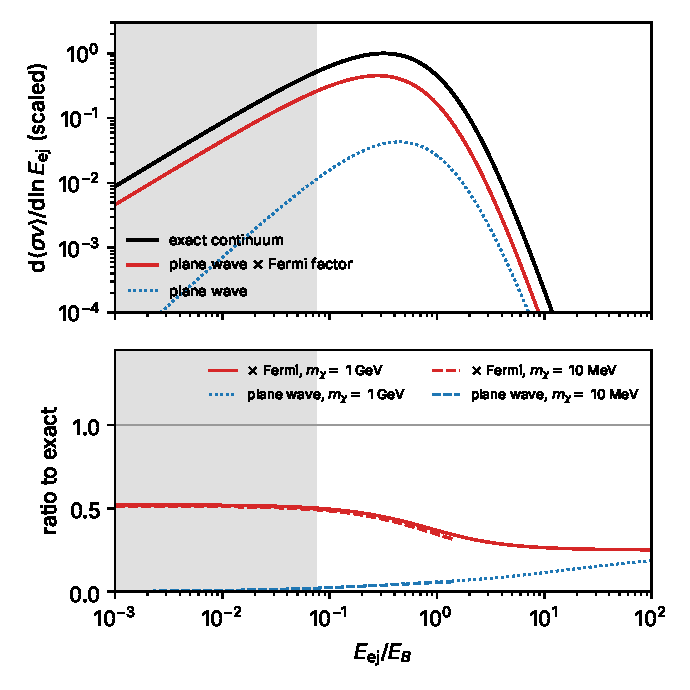
\includegraphics[width=0.8\linewidth]{figures/ch02/limit2_ionization.pdf}
\captionof{figure}{Ionization spectrum of hydrogen 1s (one electron, so half of the two-spin formula above; $E_B = \SI{13.6}{eV}$) for a heavy mediator, $\FDM = 1$, in the standard halo model with the parameters of \cref{tab:1-shm}, against $E_{\mathrm{ej}}/E_B$. Top, for $m_\chi = \SI{1}{GeV}$, scaled to the peak of the exact result: exact Coulomb continuum states (black), plane wave times the Fermi factor with $Z_{\mathrm{eff}} = 1$ (red), plane wave alone (blue dotted). Bottom: the two approximations divided by the exact spectrum, for $m_\chi = \SI{1}{GeV}$ and \SI{10}{MeV}. Gray: $E_{\mathrm{ej}} \le 0.075\,E_B$, where the Fermi-corrected plane wave reaches about half of the exact spectrum. Integrated over $E_{\mathrm{ej}}$ at \SI{1}{GeV}, it gives 0.46 of the exact rate and the plane wave alone 0.036. The exact form factor sums the overlaps with Coulomb partial waves of the hydrogen continuum.}\label{fig:2-ionization-limit}
\par}
\smallskip
Above the shaded region, where most of the rate lies, the halo forces momentum transfers $q \ge (E_B + E_{\mathrm{ej}})/v$ well above $p_{\mathrm{ej}}$, which probe the Coulomb wave at $r \sim 1/q$, where it is not a rescaled plane wave, and the approximation falls to between a quarter and a third of the exact spectrum for $E_{\mathrm{ej}}$ of several $E_B$.
\end{limitbox}

Hydrogen is the only atom with closed-form orbitals. For every other atom the initial orbitals $\psi_i$ are not known exactly: they are computed self-consistently, each electron moving in the average field of the others, as Hartree--Fock orbitals, and the ionization form factors are integrals over them. Ref.~\cite{essig2012direct} used tabulated Roothaan--Hartree--Fock wavefunctions, Hartree--Fock orbitals expanded in a finite set of analytic radial functions; \cref{app:E.7} describes how such form factors are computed and converged, and \cref{sec:3.4} makes the self-consistent-field method precise. In a crystal the same overlap is taken between Bloch states of the valence and conduction bands, summed over their crystal momenta, and the atomic $|f_{\mathrm{ion}}|^2$ becomes the crystal form factor~\cite[Eqs.~(3.13) and (3.17)]{essig2016direct} of \cref{chap:10}.

\subsection{Free electrons}

\Cref{eq:2.2-bound} contains free scattering as a special case, and the check, now in the laboratory frame, shows how the mediator mass enters the free cross-section.

\begin{workedexample}{Scattering off a free electron}\label{we:2-free}
Take an electron at rest, $|i\rangle = |\vect{0}\rangle$, with final states $|f\rangle = |\vect{k}\rangle$ in the box. By \cref{eq:2.2-ff}, $f_{i\to f}(\vect{q}) = \langle\vect{k}|\ee^{\ii\vect{q}\cdot\vect{r}}|\vect{0}\rangle = \delta_{\vect{k}\vect{q}}$: the electron takes exactly the momentum it is given. The sum over $f$ in \cref{eq:2.2-bound} keeps $\vect{k} = \vect{q}$, with $E_f - E_i = q^2/2m_e$, and with $\omega_{\vect{q}} = qv\cos\theta - q^2/2m_\chi$ the delta function is $\delta(q^2/2\mu_{\chi e} - qv\cos\theta)$, where $\theta$ is the angle between $\vect{q}$ and $\vect{v}$ and $1/\mu_{\chi e} = 1/m_e + 1/m_\chi$. Its root is $\cos\theta = q/(2\mu_{\chi e}v)$, which lies in $[-1, 1]$ for $q \le 2\mu_{\chi e}v$, and its weight is $1/(qv)$. With $\dd^3q = 2\pi q^2\,\dd q\,\dd\cos\theta$,
\begin{equation*}
  \sigma_T v = \int_0^{2\mu_{\chi e}v}\frac{2\pi q^2\,\dd q}{(2\pi)^3}\,|\tilde V(q)|^2\,\frac{2\pi}{qv}
  = \frac{1}{2\pi v}\int_0^{2\mu_{\chi e}v}q\,\dd q\,|\tilde V(q)|^2 .
\end{equation*}
Dividing by $v$ gives $\dd\sigma_T/\dd q = q|\tilde V(q)|^2/(2\pi v^2)$, which is \cref{eq:2.2-dsdq}, obtained before in the center-of-mass frame.

For a mediator of mass $m_V$, \cref{eq:1.4-yukawa-sigma} has $\FDM^2 = (m_V^2 + q_0^2)^2/(m_V^2 + q^2)^2$, and the integral over $q^2$ from $0$ to $q_{\mathrm{max}}^2 = (2\mu_{\chi e}v)^2$ is elementary, $\int_0^{q_{\mathrm{max}}^2}\dd x\,(m_V^2 + x)^{-2} = q_{\mathrm{max}}^2/[m_V^2(m_V^2 + q_{\mathrm{max}}^2)]$. So
\begin{equation*}
  \sigma_T = \sigmae\,\frac{(m_V^2 + q_0^2)^2}{m_V^2\,(m_V^2 + q_{\mathrm{max}}^2)} .
\end{equation*}
For concreteness take $m_\chi = \SI{100}{MeV}$, with $\mu_{\chi e} = \SI{0.508}{MeV}$, and the largest halo speed, $v_{\mathrm{max}} = 2.65\times10^{-3}$ (\cref{eq:1.2-vmax}). Then $q_{\mathrm{max}} = \SI{2.69}{keV} = 0.72\,q_0$. A free electron at rest cannot even absorb the reference momentum $q_0$ from such a particle: $\sigmae$ is defined at a momentum transfer that free kinematics does not reach. For a heavy mediator this does not matter. With $m_V = 10\,q_0$ we find $\sigma_T = 1.015\,\sigmae$, and at $m_V = \SI{30}{MeV}$ the difference is $2.3\times10^{-8}$. At $m_V = q_0$, $\sigma_T = 2.63\,\sigmae$, and at $m_V = 0.1\,q_0$, $\sigma_T = 192\,\sigmae$. As $m_V \to 0$ it grows as $q_0^4/(m_V^2q_{\mathrm{max}}^2)$: the free cross-section of a light mediator diverges at small $q$, like Rutherford's, and $\sigmae$ is then just a normalization (\cref{sec:1.4}).
\end{workedexample}

\noindent The free electron at rest is a poor model of a bound one. A bound electron moves with a typical speed $\sim\alpha$, about ten times the dark-matter speed (\cref{sec:1.3}), so it can absorb momentum transfers well above $2\mu_{\chi e}v$, and it needs an energy $E_f - E_i$ that free kinematics does not supply. Both effects sit in $f_{i\to f}$.

For a light mediator the bound target also removes the divergence of \cref{we:2-free}. In \cref{eq:2.2-spectrum} the factor $\FDM^2 = (q_0/q)^4$ multiplies $q\,\dd q$, and the integrand grows as $q^{-3}$ toward small $q$. It stops at $q = \omega/v_{\mathrm{max}}$, below which no dark-matter particle can deposit $\omega$. In addition, the squared form factor of every inelastic transition vanishes at small $q$, as $q^2$ for a dipole-allowed one (\cref{we:2-hydrogen}). The rate is then dominated by the smallest $q$ that kinematics allows, just above the threshold.

\subsection{Nuclei and the Helm form factor}

A nucleus of mass number $A$ is a bound target of $A$ nucleons, and \cref{eq:2.2-ff} applies with one change: every nucleon couples. With a potential $V_N(\vect{x}_\chi - \vect{r}_j)$ between the dark matter and nucleon $j$, the same for protons and neutrons, the target operator is $\sum_{j=1}^A\ee^{\ii\vect{q}\cdot\vect{r}_j}$. Write $\vect{r}_j = \vect{R}_{\mathrm{cm}} + \vect{r}'_j$, with $\vect{R}_{\mathrm{cm}}$ the center of mass of the nucleus and $\vect{r}'_j$ the internal coordinates. The center of mass is a free particle and its plane waves give momentum conservation, as in \cref{eq:2.1-Vbox}. The internal state is the nuclear ground state $|0\rangle$, before and after. The lowest excited levels lie at \SI{1.78}{MeV} in $^{28}$Si, \SI{1.27}{MeV} in $^{29}$Si and \SI{2.24}{MeV} in $^{30}$Si, and between \SI{0.56}{MeV} and \SI{1.04}{MeV} in the even germanium isotopes. The exception is $^{73}$Ge, \SI{7.8}{\percent} of natural germanium, whose first excited state is at \SI{13.3}{keV} and its second at \SI{66.7}{keV}~\cite{iaea2026livechart}. Sub-GeV dark matter carries at most a few keV of kinetic energy (\cref{sec:1.3}), below all of these. The internal matrix element is
\begin{equation}
  \Bigl\langle 0\Bigl|\sum_{j=1}^A\ee^{\ii\vect{q}\cdot\vect{r}'_j}\Bigr|0\Bigr\rangle = \int\dd^3r\;\ee^{\ii\vect{q}\cdot\vect{r}}\,\nd_N(\vect{r}) \equiv A\,F_N(q) ,
  \label{eq:2.2-FN}
\end{equation}
with $\nd_N(\vect{r})$ the nucleon number density of the nucleus, normalized to $\int\dd^3r\,\nd_N = A$, and $F_N(q)$ the \emph{nuclear form factor}, the elastic form factor of the nucleus with $F_N(0) = 1$. This is the coherent sum: at $q \to 0$ the phases of all nucleons agree and the amplitude is $A$ times that of one nucleon. The two-body result \cref{eq:2.2-dsdq}, with $\mu_{\chi e} \to \mu_{\chi N}$ and $\tilde V \to A\tilde V_N F_N$, gives
\begin{equation}
  \frac{\dd\sigma_N}{\dd q} = \frac{q\,A^2|\tilde V_N(q)|^2}{2\pi v^2}\,F_N(q)^2
  = \frac{q\,\sigma_N}{2\mu_{\chi N}^2v^2}\,F_N(q)^2 , \qquad
  \sigma_N = \frac{\mu_{\chi N}^2A^2|\tilde V_N|^2}{\pi} = \sigma_p\left(\frac{\mu_{\chi N}}{\mu_{\chi p}}\right)^2A^2 ,
  \label{eq:2.2-nucleus}
\end{equation}
for a heavy mediator, $\tilde V_N = y_\chi y_N/m_V^2$. The expression through $\sigma_p$ uses the proton cross-section $\sigma_p = \mu_{\chi p}^2|\tilde V_N|^2/\pi$, which is \cref{eq:2.2-sigma-free} with $\mu_{\chi e} \to \mu_{\chi p}$. This derives \cref{eq:1.4-sigmaN}, and $\sigma_N$ is the cross-section at $q \to 0$; the form factor then cuts off the distribution at large $q$. Unequal proton and neutron couplings replace $A$ by $Z + (A - Z)y_n/y_p$ (\cref{sec:1.4}).

Experiments measure the recoil energy $E_R = q^2/2M$ rather than $q$, with $M$ the nuclear mass. With $\dd E_R = q\,\dd q/M$, $\dd\sigma_N/\dd E_R = M\sigma_NF_N^2/(2\mu_{\chi N}^2v^2)$. We multiply by the number of nuclei per unit mass, $1/M$, and by the dark-matter flux $(\rho_\chi/m_\chi)\,v\,f_\chi(\vect{v})\,\dd^3v$. Integrating over velocities above $\vmin = (ME_R/2\mu_{\chi N}^2)^{1/2}$ (\cref{sec:1.3}) then turns the factor $v/v^2$ into $\eta(\vmin)$:
\begin{equation*}
  \frac{\dd\mathcal{R}}{\dd E_R} = \frac{\rho_\chi\,\sigma_N}{2m_\chi\mu_{\chi N}^2}\,F_N(q)^2\,\eta(\vmin) , \qquad q = (2ME_R)^{1/2} ,
\end{equation*}
the standard spin-independent recoil spectrum, Ref.~\cite[Eq.~(104)]{lin2019tasi} with $\sigma_N$ written through \cref{eq:1.4-sigmaN} and equal couplings to protons and neutrons.

The nucleon density is close to uniform inside the nucleus and falls off over a skin about \SI{1}{fm} thick. Helm's model~\cite{helm1956inelastic} writes it as a uniform sphere of radius $R_{\mathrm{nuc}}$ smeared by a Gaussian of width $s_{\mathrm{skin}}$. The transform of a convolution is the product of the transforms. For the uniform sphere, the angular integral is $4\pi\sin(qr)/(qr)$ again (\cref{app:C.3}), and $\int_0^{R}\dd r\,r\sin qr = (\sin qR - qR\cos qR)/q^2$, so its normalized transform is $3(\sin x - x\cos x)/x^3 = 3j_1(x)/x$ with $x = qR_{\mathrm{nuc}}$ and $j_1$ the spherical Bessel function. The normalized Gaussian $\ee^{-r^2/2s_{\mathrm{skin}}^2}/(2\pi s_{\mathrm{skin}}^2)^{3/2}$ transforms to $\ee^{-q^2s_{\mathrm{skin}}^2/2}$. Multiplying the two gives~\cite[Eq.~(17)]{duda2007model}
\begin{equation}
  F_{\mathrm{Helm}}(q) = \frac{3j_1(qR_{\mathrm{nuc}})}{qR_{\mathrm{nuc}}}\,\ee^{-q^2s_{\mathrm{skin}}^2/2} .
  \label{eq:2.2-helm}
\end{equation}
The standard parameters are those of Lewin and Smith~\cite{lewin1996review}: $R_{\mathrm{nuc}}^2 = c_{\mathrm{nuc}}^2 + \tfrac73\pi^2a_{\mathrm{nuc}}^2 - 5s_{\mathrm{skin}}^2$, with $c_{\mathrm{nuc}} = (1.23A^{1/3} - 0.60)\,\si{fm}$, $a_{\mathrm{nuc}} = \SI{0.52}{fm}$ and $s_{\mathrm{skin}} = \SI{0.9}{fm}$~\cite[Eqs.~(11) and (12), quoting Lewin and Smith]{duda2007model}. Here $c_{\mathrm{nuc}}$ and $a_{\mathrm{nuc}}$ are the half-density radius and surface diffuseness of a Woods--Saxon density, and the formula for $R_{\mathrm{nuc}}$ matches the Helm form to it. The literature writes $r_n$ or $R_1$ for $R_{\mathrm{nuc}}$, $s$ for $s_{\mathrm{skin}}$, and $c$, $a$ for $c_{\mathrm{nuc}}$, $a_{\mathrm{nuc}}$. At small $q$, $3j_1(x)/x \simeq 1 - x^2/10$ and $F_{\mathrm{Helm}} \simeq 1 - q^2(R_{\mathrm{nuc}}^2/10 + s_{\mathrm{skin}}^2/2)$, the form $1 - q^2\langle r^2\rangle/6$ with $\langle r^2\rangle = \tfrac35R_{\mathrm{nuc}}^2 + 3s_{\mathrm{skin}}^2$. For silicon, $c_{\mathrm{nuc}} = \SI{3.14}{fm}$ and $R_{\mathrm{nuc}} = \SI{3.47}{fm}$; for germanium ($A = 73$), $c_{\mathrm{nuc}} = \SI{4.54}{fm}$ and $R_{\mathrm{nuc}} = \SI{4.77}{fm}$. The simpler fit $R_{\mathrm{nuc}} \approx 1.14A^{1/3}$\,fm of Ref.~\cite[Sect.~IV\,C]{lin2019tasi} yields \SI{3.46}{fm} and \SI{4.76}{fm}, the same to within a percent.

The Helm form is a model, not a measurement. Electron scattering measures the charge density of the nucleus, that is, the protons. The form factor of \cref{eq:2.2-FN} needs the density of all nucleons. The standard assumption is that the two are proportional, in which case the nucleon form factor equals the charge form factor~\cite[Eqs.~(7) and (8)]{duda2007model}; for the dark photon, which couples to charge, the charge form factor is exact. The physical form factor is then the transform of the measured charge density, and Ref.~\cite[Sect.~V]{duda2007model} compares the two. For $^{28}$Si the Lewin--Smith Helm form factor differs from the measured one negligibly at small $q$ and by up to \SI{5}{\percent} at the momentum transfer of a \SI{100}{keV} recoil; for $^{70}$Ge the difference is \SI{2}{\percent} at \SI{10}{keV} and \SI{20}{\percent} at \SI{100}{keV}. We use the Helm form as the convention of the field, and it is accurate wherever light dark matter is concerned.

\begin{figure}[tbp]
  \centering
  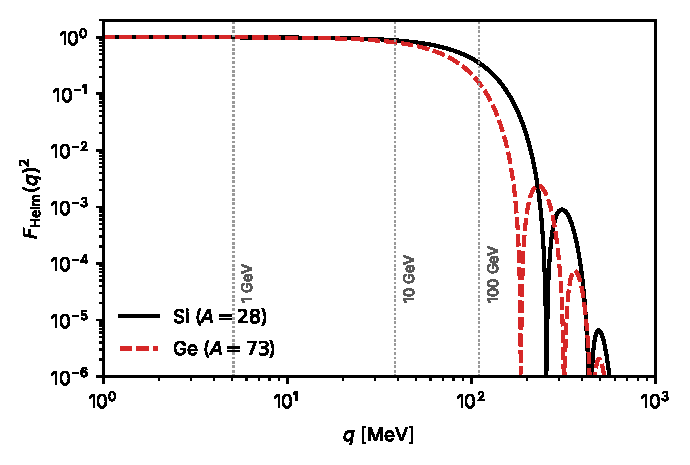
\includegraphics[width=0.62\linewidth]{figures/ch02/fig2_3.pdf}
  \caption{Squared Helm nuclear form factor $F_{\mathrm{Helm}}(q)^2 = [3j_1(qR_{\mathrm{nuc}})/(qR_{\mathrm{nuc}})]^2\ee^{-q^2s_{\mathrm{skin}}^2}$ of silicon ($A = 28$, solid) and germanium ($A = 73$, the integer nearest the mean mass number 72.6 of natural germanium; dashed), against the momentum transfer $q$. Parameters of Lewin and Smith: $R_{\mathrm{nuc}}^2 = c_{\mathrm{nuc}}^2 + \tfrac73\pi^2a_{\mathrm{nuc}}^2 - 5s_{\mathrm{skin}}^2$, $c_{\mathrm{nuc}} = (1.23A^{1/3} - 0.60)\,\si{fm}$, $a_{\mathrm{nuc}} = \SI{0.52}{fm}$, $s_{\mathrm{skin}} = \SI{0.9}{fm}$, which give $R_{\mathrm{nuc}} = \SI{3.47}{fm}$ (Si) and \SI{4.77}{fm} (Ge). Dotted lines: the maximum momentum transfer $2\mu_{\chi N}v_{\mathrm{max}}$ to a silicon nucleus for dark-matter masses of 1, 10 and \SI{100}{GeV}, with $v_{\mathrm{max}} = \SI{794.5}{km/s}$. The first zero is at $qR_{\mathrm{nuc}} = 4.49$, the first zero of $j_1$: $q = \SI{256}{MeV}$ for Si and \SI{186}{MeV} for Ge.}
  \label{fig:2-helm}
\end{figure}

\Cref{fig:2-helm} shows that light dark matter never resolves the nucleus. The silicon radius $R_{\mathrm{nuc}} = \SI{3.47}{fm}$ corresponds to $1/R_{\mathrm{nuc}} = \SI{57}{MeV}$, and germanium's \SI{4.77}{fm} to \SI{41}{MeV}. The form factor matters once $qR_{\mathrm{nuc}}$ approaches one, at tens of MeV, which needs dark matter of several GeV.

\begin{workedexample}{The $A^2$ enhancement for silicon}\label{we:2-coherent}
For $^{28}$Si, $A^2 = 784$. With the mean atomic mass of natural silicon, \SI{26.16}{GeV}, the reduced masses at $m_\chi = \SI{100}{MeV}$ are $\mu_{\chi p} = \SI{90.4}{MeV}$ and $\mu_{\chi N} = \SI{99.6}{MeV}$, and \cref{eq:2.2-nucleus} gives $\sigma_N/\sigma_p = 1.215 \times 784 = 953$; at \SI{1}{GeV}, $\mu_{\chi p} = \SI{484}{MeV}$, $\mu_{\chi N} = \SI{963}{MeV}$, and $\sigma_N/\sigma_p = 3.96 \times 784 = 3100$. Coherence turns the $A$ of 28 nucleons scattering independently into $A^2$, a gain of 28; the reduced-mass factor is a separate effect of the heavier recoiling target. Per kilogram of target the rate still grows as $A$, because $A^2$ in the cross-section beats the $1/A$ in the number of nuclei per unit mass. The form factor costs almost nothing. At $m_\chi = \SI{1}{GeV}$ the maximum momentum transfer is $q_{\mathrm{max}} = 2\mu_{\chi N}v_{\mathrm{max}} = \SI{5.10}{MeV}$ (\cref{we:1-nuclear}), and $q_{\mathrm{max}}R_{\mathrm{nuc}} = 0.090$ and $F_{\mathrm{Helm}}^2 = 0.998$ at the maximum momentum transfer, where the suppression is greatest. The same calculation yields $F_{\mathrm{Helm}}^2(q_{\mathrm{max}}) = 0.89$ at \SI{10}{GeV} and $0.36$ at \SI{100}{GeV}. For germanium at \SI{100}{GeV}, $q_{\mathrm{max}} = \SI{214}{MeV}$ lies beyond the first zero and $F_{\mathrm{Helm}}^2 = 0.002$ there. Form factors shape the recoil spectra of weak-scale dark matter but are a \SI{0.2}{\percent} correction at \SI{1}{GeV} and far less for the sub-GeV dark matter of this book.
\end{workedexample}

\section{Second quantization}\label{sec:2.3}

When dark matter lifts one electron of silicon across the gap, the other $10^{26}$ electrons stay where they were. Written as a wave function, the final state is still an antisymmetric function of all the electron coordinates, and so is the ground state. Written as a list of which single-particle orbitals are filled, the two states differ in two entries: one orbital emptied, one filled. Second quantization is the bookkeeping that works with such lists. Its operators create and destroy particles in orbitals, they take care of the exchange signs automatically, and every operator we need, from the density $n_e(\vect{q})$ that dark matter couples to, to the Coulomb Hamiltonian of electrons and nuclei, takes a compact form in them. Phonons and magnons later fit into the same language (\cref{sec:5.3,sec:7.1}). We follow the standard treatments of Refs.~\cite[Chap.~1]{bruus2004many}, \cite[Chap.~1]{fetter1971quantum} and \cite[Chap.~1]{giuliani2005quantum}.

\subsection{Identical particles}

Two electrons cannot be told apart, and swapping their labels changes no measurement. Write $x_i = (\vect{r}_i, s_i)$ for the position and spin projection $s_i = {\uparrow},{\downarrow}$ of particle $i$. The $N$-particle wave function $\Psi(x_1,\dots,x_N)$ can then change under the exchange of two arguments only by a phase, and for the particles of this book that phase is $+1$ or $-1$. Electrons, and fermions generally, take $-1$: $\Psi$ is antisymmetric under every exchange. Bosons, such as phonons and photons, take $+1$.

For particles that do not interact, the eigenstates are built from single-particle orbitals $\psi_\gamma(x) = \langle x|\gamma\rangle$, where $\gamma$ labels a complete orthonormal set of one-particle states, spin included: plane waves $\gamma = (\vect{k}, s)$ in a box, atomic orbitals, or the Bloch states of \cref{sec:3.2}. The product $\psi_{\gamma_1}(x_1)\cdots\psi_{\gamma_N}(x_N)$ is not antisymmetric. Summing it over all permutations $P$ of the arguments, with the sign $(-1)^P$ of each, fixes that and gives the Slater determinant
\begin{equation}
  \Psi_{\gamma_1\dots\gamma_N}(x_1,\dots,x_N) = \frac{1}{\sqrt{N!}}\sum_P (-1)^P\,\psi_{\gamma_1}(x_{P1})\cdots\psi_{\gamma_N}(x_{PN})
  = \frac{1}{\sqrt{N!}}\det\bigl[\psi_{\gamma_j}(x_i)\bigr] .
  \label{eq:2.3-slater}
\end{equation}
Two equal labels give two equal columns, and the determinant vanishes: this is the Pauli principle. Swapping two labels swaps two columns and flips the sign. Orthonormal orbitals make $\Psi$ normalized, and Slater determinants with different sets of labels are orthogonal. The determinants built from all $N$-element subsets of the labels form a basis of the antisymmetric $N$-particle states, interacting or not. A correlated ground state is a superposition of many of them.

A determinant is fixed, up to its sign, by which orbitals it contains. We therefore fix an order of the labels once and for all, and write the state as a list of occupation numbers,
\begin{equation*}
  |n_{\gamma_1}, n_{\gamma_2}, n_{\gamma_3},\dots\rangle, \qquad n_\gamma \in \{0, 1\},
\end{equation*}
with the determinant's columns in the fixed order. For bosons the same construction uses the permanent (all signs $+$), any $n_\gamma \ge 0$ is allowed, and a normalization factor $(\prod_\gamma n_\gamma!)^{-1/2}$ is needed because repeated labels make some permutations identical. The space spanned by the occupation-number states of every total number $N = 0, 1, 2, \dots$ is Fock space. Its state with no particles is the vacuum $|0\rangle$. Fock space lets the particle number change, which the operators below need even when the physical number of electrons is fixed: removing an electron and putting it back elsewhere passes through the space with one electron fewer.

\subsection{Fermion operators}

The creation operator $c^\dagger_\gamma$ adds an electron in orbital $\gamma$ and puts it at the front of the list:
\begin{equation}
  c^\dagger_\gamma\,|\gamma_1\dots\gamma_N\rangle = |\gamma\,\gamma_1\dots\gamma_N\rangle ,
  \label{eq:2.3-cdag}
\end{equation}
where $|\gamma_1\dots\gamma_N\rangle$ is the determinant of \cref{eq:2.3-slater} as a ket. Every determinant is then a string of creation operators acting on the vacuum, $|\gamma_1\dots\gamma_N\rangle = c^\dagger_{\gamma_1}c^\dagger_{\gamma_2}\cdots c^\dagger_{\gamma_N}|0\rangle$. Since swapping two labels flips the sign of the determinant, $c^\dagger_\gamma c^\dagger_{\gamma'} = -c^\dagger_{\gamma'}c^\dagger_\gamma$, and in particular $(c^\dagger_\gamma)^2 = 0$. The annihilation operator $c_\gamma$ is the adjoint of $c^\dagger_\gamma$.

To see what $c_\gamma$ does, act on an occupation-number state. Let $S_\gamma = \sum_{\gamma' < \gamma}n_{\gamma'}$ count the occupied orbitals that come before $\gamma$ in the fixed order. To bring a new electron in $\gamma$ from the front of the string to its own place, $c^\dagger_\gamma$ must pass $S_\gamma$ creation operators. Since each pass costs a sign,
\begin{equation}
\begin{aligned}
  c^\dagger_\gamma\,|\dots n_\gamma\dots\rangle &= (-1)^{S_\gamma}\,(1 - n_\gamma)\,|\dots 1_\gamma\dots\rangle,\\
  c_\gamma\,|\dots n_\gamma\dots\rangle &= (-1)^{S_\gamma}\,n_\gamma\,|\dots 0_\gamma\dots\rangle .
\end{aligned}
  \label{eq:2.3-action}
\end{equation}
The second relation follows from the first: the only nonzero matrix element of $c^\dagger_\gamma$ takes $0_\gamma$ to $1_\gamma$ and equals $(-1)^{S_\gamma}$, and its complex conjugate is the matrix element of $c_\gamma$ between the same states in the other direction. In words, $c_\gamma$ empties a full orbital and kills an empty one, and neither operator can act twice on the same orbital.

The algebra follows in two lines. For $\gamma = \gamma'$, \cref{eq:2.3-action} leads to $c_\gamma c^\dagger_\gamma|\dots n_\gamma\dots\rangle = (1 - n_\gamma)|\dots n_\gamma\dots\rangle$ and $c^\dagger_\gamma c_\gamma|\dots n_\gamma\dots\rangle = n_\gamma|\dots n_\gamma\dots\rangle$, and the two add to one. For $\gamma \ne \gamma'$, the two orders of $c_\gamma$ and $c^\dagger_{\gamma'}$ reach the same final state, but in one of them the second operator sees the occupation of the other orbital changed by one, and the sign factors differ by $-1$. With $\{A, B\} = AB + BA$,
\begin{equation}
  \{c_\gamma, c^\dagger_{\gamma'}\} = \delta_{\gamma\gamma'}, \qquad \{c_\gamma, c_{\gamma'}\} = \{c^\dagger_\gamma, c^\dagger_{\gamma'}\} = 0 .
  \label{eq:2.3-anticomm}
\end{equation}
These anticommutation relations contain the whole of Fermi statistics: the Pauli principle is $(c^\dagger_\gamma)^2 = 0$, and the exchange signs of \cref{eq:2.3-slater} are the signs picked up by reordering operators.

The product $c^\dagger_\gamma c_\gamma$ counts the electrons in $\gamma$: its eigenvalue on $|\dots n_\gamma\dots\rangle$ is $n_\gamma$. The total number operator is $\op{N}_e = \sum_\gamma c^\dagger_\gamma c_\gamma$, with eigenvalue $N_e$ on every state with $N_e$ electrons. A Hamiltonian of independent electrons with orbital energies $E_\gamma$ is $\sum_\gamma E_\gamma\,c^\dagger_\gamma c_\gamma$: each filled orbital adds its energy. The excitation of the opening paragraph, an electron moved from a filled orbital $\gamma_v$ to an empty one $\gamma_c$, is $c^\dagger_{\gamma_c}c_{\gamma_v}$ acting on the ground state, and its energy is $E_{\gamma_c} - E_{\gamma_v}$ in this approximation.

The commutator of a bilinear with a single operator does most of the work later. By \cref{eq:2.3-anticomm},
\begin{equation}
  [c^\dagger_\gamma c_{\gamma'},\, c^\dagger_{\gamma''}] = \delta_{\gamma'\gamma''}\,c^\dagger_\gamma , \qquad
  [c^\dagger_\gamma c_{\gamma'},\, c_{\gamma''}] = -\delta_{\gamma\gamma''}\,c_{\gamma'} ,
  \label{eq:2.3-bilinear}
\end{equation}
because $c^\dagger_\gamma c_{\gamma'}c^\dagger_{\gamma''} = \delta_{\gamma'\gamma''}c^\dagger_\gamma - c^\dagger_\gamma c^\dagger_{\gamma''}c_{\gamma'}$ and the last term equals $-c^\dagger_{\gamma''}c^\dagger_\gamma c_{\gamma'}$ after one swap of creation operators. The sign problems of fermions cancel in pairs here: a bilinear behaves like an ordinary operator that moves one particle. As a result, every bilinear commutes with $\op{N}_e$, and operators built from bilinears conserve the number of electrons. And for independent electrons, $H_0 = \sum_\gamma E_\gamma c^\dagger_\gamma c_\gamma$, the Heisenberg equation $\ii\,\dd c^\dagger_\gamma/\dd t = [c^\dagger_\gamma, H_0] = -E_\gamma c^\dagger_\gamma$ integrates to $\ee^{\ii H_0t}c^\dagger_\gamma\ee^{-\ii H_0t} = \ee^{\ii E_\gamma t}c^\dagger_\gamma$. An operator that moves an electron from $\gamma'$ to $\gamma$ then oscillates as $\ee^{\ii(E_\gamma - E_{\gamma'})t}$, at the energy of the transition it causes, which is how the energy denominators of \cref{sec:2.4} and the response functions of \cref{sec:4.1} arise.

\subsection{Boson operators}

Bosons work the same way with every sign turned positive. Generic boson operators $d_\gamma$, $d^\dagger_\gamma$ act on occupation numbers $n_\gamma = 0, 1, 2, \dots$ as
\begin{equation}
  d^\dagger_\gamma\,|\dots n_\gamma\dots\rangle = \sqrt{n_\gamma + 1}\,|\dots n_\gamma + 1\dots\rangle, \qquad
  d_\gamma\,|\dots n_\gamma\dots\rangle = \sqrt{n_\gamma}\,|\dots n_\gamma - 1\dots\rangle ,
  \label{eq:2.3-boson}
\end{equation}
with no sign factor, because exchanging bosons costs nothing. The square roots come from the normalization factor of the symmetrized states: the state with $n_\gamma + 1$ quanta, built by $d^\dagger_\gamma$ from the state with $n_\gamma$, has norm $n_\gamma + 1$ before it is normalized. Then $d_\gamma d^\dagger_\gamma - d^\dagger_\gamma d_\gamma$ gives $(n_\gamma + 1) - n_\gamma = 1$ on every state, and operators of different modes commute:
\begin{equation}
  [d_\gamma, d^\dagger_{\gamma'}] = \delta_{\gamma\gamma'}, \qquad [d_\gamma, d_{\gamma'}] = [d^\dagger_\gamma, d^\dagger_{\gamma'}] = 0 .
  \label{eq:2.3-comm}
\end{equation}
The number of quanta in mode $\gamma$ is $d^\dagger_\gamma d_\gamma$.

These are the ladder operators of the harmonic oscillator. An oscillator of frequency $E_\gamma$ has $H = E_\gamma(d^\dagger_\gamma d_\gamma + \tfrac12)$, and its $n$th level reads as $n$ quanta in a single mode. A set of uncoupled oscillators, such as the normal modes of a crystal, is a set of bosonic modes. This is why the quantized lattice vibrations of \cref{sec:5.3} are particles, phonons, with operators $b_{\vect{Q}\nu}$. The magnon operators $a_{\vect{k}\nu}$ of \cref{sec:7.1} are bosons in the same sense. \Cref{eq:2.3-boson} is the origin of the matrix elements $\sqrt{n}$ for absorption and $\sqrt{n + 1}$ for emission quoted in \cref{sec:2.1}, and \cref{sec:2.5} puts thermal occupations into $n$.

Unlike electrons, these bosons are created and destroyed in physical processes, and the Hamiltonians that describe this are not built from bilinears $d^\dagger d$ alone. An electron that emits or absorbs a phonon is described by a term of the form $c^\dagger_{\gamma}c_{\gamma'}(b_{\vect{Q}\nu} + b^\dagger_{-\vect{Q}\nu})$, with phonon wavevector $\vect{Q}$ and branch $\nu$ (\cref{sec:6.2}): the electron bilinear conserves electron number and the boson operator changes the number of phonons by one. Absorption of bosonic dark matter fits the same pattern. If the dark-matter field is quantized, the oscillating amplitude $\phi_0$ of \cref{sec:2.1} becomes an annihilation operator for the dark-matter mode. Its matrix element $\sqrt{n}$ between states with $n$ and $n - 1$ quanta leads to a rate proportional to the number of quanta in the mode, that is, to the density $\rho_\chi$. The classical field of \cref{sec:2.1} is the limit of large $n$, where $\sqrt{n}$ and $\sqrt{n+1}$ no longer differ.

\subsection{One-body operators and the density}

The operator that dark matter couples to in electron scattering is $n_e(\vect{q}) = \sum_i\ee^{\ii\vect{q}\cdot\vect{r}_i}$ (\cref{eq:A.3-ne}). It is a sum over electrons of the same single-particle operator, and so are the kinetic energy $\sum_i\vect{p}_i^2/2m_e$ and the potential energy $\sum_i U_1(\vect{r}_i)$ in an external potential $U_1$. A one-body operator has this form, $\op{O}_1 = \sum_i\op{o}_i$, where $\op{o}_i$ is a fixed one-particle operator $\op{o}$ acting on particle $i$. In Fock space it reads
\begin{keyresult}[One-body operators]
\begin{equation}
  \op{O}_1 = \sum_{i=1}^{N}\op{o}_i \;=\; \sum_{\gamma\gamma'}\langle\gamma|\op{o}|\gamma'\rangle\,c^\dagger_\gamma c_{\gamma'} .
  \label{eq:2.3-onebody}
\end{equation}
The right-hand side is the same for every $N$, holds for bosons with $c \to d$, and has the same form in every orthonormal single-particle basis.
\end{keyresult}
Acting on a determinant, $\sum_i\op{o}_i$ replaces each occupied orbital in turn by $\op{o}|\gamma_j\rangle = \sum_\gamma|\gamma\rangle\langle\gamma|\op{o}|\gamma_j\rangle$ and leaves the rest alone, and the bilinear $c^\dagger_\gamma c_{\gamma_j}$ does exactly this replacement. \Cref{app:D.2} writes out this argument, extends it to bosons, and proves the basis independence stated in the box.

Expressed through the field operator,
\begin{equation}
  \op{\psi}_s(\vect{r}) = \sum_\gamma\psi_\gamma(\vect{r}, s)\,c_\gamma ,
  \qquad \{\op{\psi}_s(\vect{r}), \op{\psi}^\dagger_{s'}(\vect{r}')\} = \delta_{ss'}\,\delta^3(\vect{r} - \vect{r}') ,
  \label{eq:2.3-field}
\end{equation}
\cref{eq:2.3-onebody} takes a basis-free form. The anticommutator follows from \cref{eq:2.3-anticomm} and the completeness of the orbitals, $\sum_\gamma\psi_\gamma(\vect{r}, s)\psi^*_\gamma(\vect{r}', s') = \delta_{ss'}\delta^3(\vect{r} - \vect{r}')$. We see that $\op{\psi}^\dagger_s(\vect{r})$ creates an electron at the point $\vect{r}$ with spin $s$, and the density of electrons at $\vect{r}$, written $\nd_e(\vect{r}) = \sum_i\delta^3(\vect{r} - \vect{r}_i)$ in \cref{app:A.3}, becomes $\sum_s\op{\psi}^\dagger_s(\vect{r})\op{\psi}_s(\vect{r})$. For an operator that is local in position and spin-independent, such as $\ee^{\ii\vect{q}\cdot\vect{r}}$ or $U_1(\vect{r})$, \cref{eq:2.3-onebody} becomes $\sum_s\int\dd^3r\,\op{\psi}^\dagger_s(\vect{r})\,o(\vect{r})\,\op{\psi}_s(\vect{r})$; the kinetic energy puts $-\nabla^2/2m_e$ between the two field operators.

In a box with plane waves, $\psi_{\vect{k}s}(\vect{r}, s') = \delta_{ss'}\ee^{\ii\vect{k}\cdot\vect{r}}/\sqrt{\Vol}$ (\cref{eq:2.1-box}), and the field operator is $\op{\psi}_s(\vect{r}) = \Vol^{-1/2}\sum_{\vect{k}}\ee^{\ii\vect{k}\cdot\vect{r}}\,c_{\vect{k}s}$. The matrix element of the density is a Kronecker delta,
\begin{equation*}
  \langle\vect{k}'s'|\ee^{\ii\vect{q}\cdot\vect{r}}|\vect{k}s\rangle = \frac{\delta_{ss'}}{\Vol}\int\dd^3r\,\ee^{\ii(\vect{k} + \vect{q} - \vect{k}')\cdot\vect{r}} = \delta_{\vect{k}',\vect{k}+\vect{q}}\,\delta_{ss'} ,
\end{equation*}
so
\begin{equation}
  n_e(\vect{q}) = \sum_{\gamma\gamma'}\langle\gamma|\ee^{\ii\vect{q}\cdot\vect{r}}|\gamma'\rangle\,c^\dagger_\gamma c_{\gamma'}
  = \sum_{\vect{k}s}c^\dagger_{\vect{k}+\vect{q},s}\,c_{\vect{k}s} .
  \label{eq:2.3-nq}
\end{equation}
The density operator takes an electron from $\vect{k}$ and puts it at $\vect{k} + \vect{q}$, keeping its spin. That is the momentum bookkeeping of a scattering event: the dark matter goes from $\vect{p}$ to $\vect{p} - \vect{q}$, and \cref{eq:A.3-vertex} shows that its interaction with the electrons, between these two dark-matter states, is $\tilde V(\vect{q})\,n_e(\vect{q})/\Vol$. We can therefore write every electronic scattering rate of this book as a matrix element of $n_e(\vect{q})$ between many-electron states, squared and summed (\cref{sec:4.2}). Note that $n_e(\vect{q})^\dagger = n_e(-\vect{q})$, and that $n_e(\vect{0}) = \op{N}_e$. In a crystal the same formula in the Bloch basis gives the density vertex of \cref{sec:3.2}.

The plane-wave form also shows the Pauli principle at work in a scattering event. Acting on a state in which the electrons fill all plane waves inside some region of $\vect{k}$ space, the term $c^\dagger_{\vect{k}+\vect{q},s}c_{\vect{k}s}$ survives only if $\vect{k}$ is filled and $\vect{k} + \vect{q}$ is empty. For a momentum transfer $q$ small compared with the size of the filled region, only electrons within about $q$ of its surface can take the momentum, and the rest are blocked. This is why the electrons of a metal respond to slow dark matter as a thin shell rather than as the whole electron density, a point \cref{sec:2.5,sec:4.5} make quantitative. At $q$ larger than the filled region no electron is blocked, and every term contributes. The same counting, with the filled region replaced by the valence bands and the empty one by the conduction bands, sets the electronic excitations of a semiconductor.

For independent electrons the many-body matrix element of $n_e(\vect{q})$ reduces to a single-particle one. Let $|\Phi_0\rangle$ be a determinant with orbital $\gamma_v$ filled and $\gamma_c$ empty, and $c^\dagger_{\gamma_c}c_{\gamma_v}|\Phi_0\rangle$ the excited determinant, whose bra is $\langle\Phi_0|c^\dagger_{\gamma_v}c_{\gamma_c}$. In $\langle\Phi_0|c^\dagger_{\gamma_v}c_{\gamma_c}\,c^\dagger_\gamma c_{\gamma'}|\Phi_0\rangle$ the bilinear $c^\dagger_\gamma c_{\gamma'}$ must undo the excitation, and only $\gamma = \gamma_c$, $\gamma' = \gamma_v$ survives, with weight one. With \cref{eq:2.3-nq},
\begin{equation}
  \langle\Phi_0|c^\dagger_{\gamma_v}c_{\gamma_c}\;n_e(\vect{q})\;|\Phi_0\rangle = \langle\gamma_c|\ee^{\ii\vect{q}\cdot\vect{r}}|\gamma_v\rangle ,
  \label{eq:2.3-ph}
\end{equation}
which is the transition form factor $f_{i\to f}(\vect{q})$ of \cref{sec:2.2} for the electron that moves, whatever the other electrons do. The spectators enter only through which orbitals are blocked. Interactions spoil this simple picture, and \cref{sec:4.2,sec:4.6} show what replaces it.

A one-body potential follows from the inverse transform. With \cref{eq:A.3-space,eq:A.3-box}, $U_1(\vect{r}) = \Vol^{-1}\sum_{\vect{q}}\ee^{-\ii\vect{q}\cdot\vect{r}}U_1(\vect{q})$, and $\sum_iU_1(\vect{r}_i) = \Vol^{-1}\sum_{\vect{q}}U_1(\vect{q})\,n_e(-\vect{q})$: a potential with a Fourier component at $\vect{q}$ moves electrons by $-\vect{q}$. For plane waves the kinetic energy is diagonal, $\sum_{\vect{k}s}(k^2/2m_e)\,c^\dagger_{\vect{k}s}c_{\vect{k}s}$. \Cref{tab:2-operators} collects these forms with the two-body operators derived below.

\begin{table}[tbp]
  \centering
  \small
  \caption{Operators used in this book in first quantization (sums over electrons $i$ and nuclei $I$) and in second quantization, in a general orthonormal single-particle basis $\{|\gamma\rangle\}$ (spin included in $\gamma$) and in box-normalized plane waves $|\vect{k}s\rangle$ of a box of volume $\Vol$. Fourier transforms carry $\ee^{+\ii\vect{q}\cdot\vect{r}}$; $v_{\mathrm{C}}(k) = e^2/k^2$ is the Heaviside--Lorentz Coulomb kernel, $e^2 = 4\pi\alpha$; $Z_\kappa$ is the charge number of nuclear species $\kappa$ and $n_\kappa(\vect{k}) = \sum_{I\in\kappa}\ee^{\ii\vect{k}\cdot\vect{X}_I}$ its density, with $\vect{X}_I$ the position of nucleus $I$. Two-body elements are $\langle\gamma_1\gamma_2|U_2|\gamma_3\gamma_4\rangle = \int\dd x\,\dd x'\,\psi^*_{\gamma_1}(x)\psi^*_{\gamma_2}(x')U_2(\vect{r} - \vect{r}')\psi_{\gamma_3}(x)\psi_{\gamma_4}(x')$, with $x = (\vect{r}, s)$ and $\int\dd x = \sum_s\int\dd^3r$. The $\vect{k} = 0$ Coulomb terms are removed by charge neutrality (\cref{we:2-jellium}).}
  \label{tab:2-operators}
  \renewcommand{\arraystretch}{1.5}
  \begin{tabular}{@{}p{0.27\linewidth}p{0.30\linewidth}p{0.37\linewidth}@{}}
    \toprule
    First quantization & General basis & Plane waves \\
    \midrule
    $N_e = \sum_i 1$ & $\op{N}_e = \sum_\gamma c^\dagger_\gamma c_\gamma$ & $\sum_{\vect{k}s}c^\dagger_{\vect{k}s}c_{\vect{k}s}$ \\
    $\sum_i\vect{p}_i^2/2m_e$ & $\sum_{\gamma\gamma'}\langle\gamma|\tfrac{\vect{p}^2}{2m_e}|\gamma'\rangle c^\dagger_\gamma c_{\gamma'}$ & $\sum_{\vect{k}s}\tfrac{k^2}{2m_e}c^\dagger_{\vect{k}s}c_{\vect{k}s}$ \\
    $\sum_iU_1(\vect{r}_i)$ & $\sum_{\gamma\gamma'}\langle\gamma|U_1|\gamma'\rangle c^\dagger_\gamma c_{\gamma'}$ & $\tfrac1\Vol\sum_{\vect{q}}U_1(\vect{q})\,n_e(-\vect{q})$ \\
    $n_e(\vect{q}) = \sum_i\ee^{\ii\vect{q}\cdot\vect{r}_i}$ & $\sum_{\gamma\gamma'}\langle\gamma|\ee^{\ii\vect{q}\cdot\vect{r}}|\gamma'\rangle c^\dagger_\gamma c_{\gamma'}$ & $\sum_{\vect{k}s}c^\dagger_{\vect{k}+\vect{q},s}c_{\vect{k}s}$ \\
    dark matter $\vect{p} \to \vect{p} - \vect{q}$: $\tfrac1\Vol\tilde V(\vect{q})\sum_i\ee^{\ii\vect{q}\cdot\vect{r}_i}$ & $\tfrac1\Vol\tilde V(\vect{q})\,n_e(\vect{q})$ & $\tfrac1\Vol\tilde V(\vect{q})\sum_{\vect{k}s}c^\dagger_{\vect{k}+\vect{q},s}c_{\vect{k}s}$ \\
    $\tfrac12\sum_{i\ne j}U_2(\vect{r}_i - \vect{r}_j)$ & $\tfrac12\sum\langle\gamma_1\gamma_2|U_2|\gamma_3\gamma_4\rangle$\newline$\quad\times c^\dagger_{\gamma_1}c^\dagger_{\gamma_2}c_{\gamma_4}c_{\gamma_3}$ & $\tfrac1{2\Vol}\sum_{\vect{k}\vect{p}\vect{p}'ss'}U_2(\vect{k})$\newline$\quad\times c^\dagger_{\vect{p}+\vect{k},s}c^\dagger_{\vect{p}'-\vect{k},s'}c_{\vect{p}'s'}c_{\vect{p}s}$ \\
    $\sum_{i<j}\dfrac{e^2}{4\pi|\vect{r}_i - \vect{r}_j|}$ & $U_2 \to e^2/(4\pi|\vect{r} - \vect{r}'|)$ & $\tfrac1{2\Vol}\sum_{\vect{k}\ne0}v_{\mathrm{C}}(k)\bigl[n_e(\vect{k})^\dagger n_e(\vect{k}) - \op{N}_e\bigr]$ \\
    $-\sum_{iI}\dfrac{Z_{\kappa(I)}e^2}{4\pi|\vect{r}_i - \vect{X}_I|}$ & $\sum_{\gamma\gamma'}\langle\gamma|U_1|\gamma'\rangle c^\dagger_\gamma c_{\gamma'}$, $U_1(\vect{r}) = -\sum_I\dfrac{Z_{\kappa(I)}e^2}{4\pi|\vect{r} - \vect{X}_I|}$ & $-\tfrac1\Vol\sum_{\vect{k}\ne0}v_{\mathrm{C}}(k)\sum_\kappa Z_\kappa\,n_\kappa(\vect{k})\,n_e(\vect{k})^\dagger$ \\
    \bottomrule
  \end{tabular}
\end{table}

\subsection{Change of basis}

A calculation often starts in one basis and ends in another: plane waves for the Coulomb interaction, Bloch states for the band structure (\cref{sec:3.2}), localized Wannier orbitals for interpolation (\cref{sec:3.6}). A new orthonormal basis $|\tilde\gamma\rangle = \sum_\gamma|\gamma\rangle\langle\gamma|\tilde\gamma\rangle$ comes with new operators, defined by the same rule. A creation operator adds a particle in a given orbital, so it expands like the orbital:
\begin{equation}
  c^\dagger_{\tilde\gamma} = \sum_\gamma\langle\gamma|\tilde\gamma\rangle\,c^\dagger_\gamma , \qquad
  c_{\tilde\gamma} = \sum_\gamma\langle\tilde\gamma|\gamma\rangle\,c_\gamma .
  \label{eq:2.3-basis}
\end{equation}
The coefficients form a unitary matrix, so the anticommutators survive,
\begin{equation*}
  \{c_{\tilde\gamma}, c^\dagger_{\tilde\gamma'}\} = \sum_\gamma\langle\tilde\gamma|\gamma\rangle\langle\gamma|\tilde\gamma'\rangle = \delta_{\tilde\gamma\tilde\gamma'} .
\end{equation*}
Inserting \cref{eq:2.3-basis} into \cref{eq:2.3-onebody} and using completeness twice leads to $\sum_{\tilde\gamma\tilde\gamma'}\langle\tilde\gamma|\op{o}|\tilde\gamma'\rangle c^\dagger_{\tilde\gamma}c_{\tilde\gamma'}$: one-body operators look the same in every basis, with the matrix elements of the new one. The field operator of \cref{eq:2.3-field} is the special case in which the new basis is the position eigenbasis, $\langle\gamma|\vect{r}s\rangle = \psi^*_\gamma(\vect{r}, s)$. In the basis that diagonalizes $\op{o}$ the bilinear collapses to $\sum_\gamma o_\gamma c^\dagger_\gamma c_\gamma$. A Slater determinant in the old basis becomes a sum of determinants in the new one (\cref{app:D.2}), which is why the occupation-number language, and not the wave function, is the economical one.

Take two orthonormal orbitals $|A\rangle$ and $|B\rangle$, one on each of two neighboring atoms, and the bonding and antibonding combinations $|\pm\rangle = (|A\rangle \pm |B\rangle)/\sqrt2$, a caricature of the covalent bond of silicon. Two electrons of opposite spin in the bonding orbital form one determinant, $c^\dagger_{+\uparrow}c^\dagger_{+\downarrow}|0\rangle$. By \cref{eq:2.3-basis} it is
\begin{equation*}
  c^\dagger_{+\uparrow}c^\dagger_{+\downarrow}|0\rangle
  = \tfrac12\bigl(c^\dagger_{A\uparrow}c^\dagger_{A\downarrow} + c^\dagger_{B\uparrow}c^\dagger_{B\downarrow}
  + c^\dagger_{A\uparrow}c^\dagger_{B\downarrow} + c^\dagger_{B\uparrow}c^\dagger_{A\downarrow}\bigr)|0\rangle ,
\end{equation*}
four determinants in the atomic basis: two with both electrons on one atom, and two with one electron on each. The same state is simple in one basis and a superposition in the other, and the operators of \cref{eq:2.3-onebody,eq:2.3-twobody} handle both without any change of form.

\subsection{Two-body operators and normal ordering}

The Coulomb repulsion $\tfrac12\sum_{i\ne j}U_2(\vect{r}_i - \vect{r}_j)$, with $U_2(\vect{r}) = e^2/(4\pi r)$, is a sum over pairs, and the condition $i \ne j$ matters: an electron does not repel itself. To see what it becomes, split the pair sum into all pairs minus the diagonal, $\sum_{i\ne j} = \sum_{i,j} - \sum_{i=j}$, and write each sum through the density $\nd_e(\vect{r}) = \sum_i\delta^3(\vect{r} - \vect{r}_i)$:
\begin{equation*}
  \frac12\sum_{i\ne j}U_2(\vect{r}_i - \vect{r}_j)
  = \frac12\int\dd^3r\,\dd^3r'\,U_2(\vect{r} - \vect{r}')\bigl[\nd_e(\vect{r})\nd_e(\vect{r}') - \delta^3(\vect{r} - \vect{r}')\,\nd_e(\vect{r})\bigr] .
\end{equation*}
Each density is now the bilinear $\sum_s\op{\psi}^\dagger_s\op{\psi}_s$. Moving the inner annihilation operator in $\op{\psi}^\dagger_s(\vect{r})\op{\psi}_s(\vect{r})\op{\psi}^\dagger_{s'}(\vect{r}')\op{\psi}_{s'}(\vect{r}')$ to the right with \cref{eq:2.3-field} produces a term $\delta_{ss'}\delta^3(\vect{r} - \vect{r}')\op{\psi}^\dagger_s(\vect{r})\op{\psi}_{s}(\vect{r})$, which cancels the self-interaction term exactly, and leaves, for $\op{O}_2 = \tfrac12\sum_{i\ne j}U_2(\vect{r}_i - \vect{r}_j)$,
\begin{equation}
  \op{O}_2 = \frac12\sum_{ss'}\int\dd^3r\,\dd^3r'\,U_2(\vect{r} - \vect{r}')\,\op{\psi}^\dagger_s(\vect{r})\op{\psi}^\dagger_{s'}(\vect{r}')\op{\psi}_{s'}(\vect{r}')\op{\psi}_s(\vect{r}) .
  \label{eq:2.3-twobody-field}
\end{equation}
All creation operators stand to the left of all annihilation operators. An operator product rearranged into this order, with the sign of the permutation for fermions, is called normal ordered and is written $:\!\cdots\!:$. Thus $\op{O}_2 = \tfrac12\int\!\int U_2\,{:}\nd_e(\vect{r})\nd_e(\vect{r}'){:}$, and normal ordering is what removes the self-interaction. Since a normal-ordered product of two annihilation operators vanishes on any state with fewer than two particles, a single electron feels no Coulomb energy of its own, as it should, and the vacuum has none either. Expanding the field operators in a basis gives the general form of \cref{tab:2-operators},
\begin{equation}
  \op{O}_2 = \frac12\sum_{\gamma_1\gamma_2\gamma_3\gamma_4}\langle\gamma_1\gamma_2|U_2|\gamma_3\gamma_4\rangle\,c^\dagger_{\gamma_1}c^\dagger_{\gamma_2}c_{\gamma_4}c_{\gamma_3} .
  \label{eq:2.3-twobody}
\end{equation}
The order of the last two indices matters: particle 2 is annihilated first and created last, so the two operators of each particle sit symmetrically around the middle. Reversing them flips the sign. \Cref{app:D.2} proves \cref{eq:2.3-twobody} for any two-body operator, spin-dependent or not, by applying the one-body result twice, which is the operator form of the split $\sum_{i,j} - \sum_{i=j}$ used above.

\subsection{Coulomb interaction in momentum space}

The Coulomb potential $e^2/(4\pi r)$ has the Fourier transform (\cref{eq:A.2-vC})
\begin{equation}
  v_{\mathrm{C}}(k) = \frac{e^2}{k^2} = \frac{4\pi\alpha}{k^2} \qquad \text{(Heaviside--Lorentz)} ,
  \label{eq:2.3-vC}
\end{equation}
the $m_V \to 0$ limit of the Yukawa transform of \cref{eq:C.9-Gq}. In Gaussian units the same kernel reads $4\pi e_{\mathrm{G}}^2/k^2$, and in SI units $e_{\mathrm{SI}}^2/(\varepsilon_0^{\mathrm{SI}}k^2)$ (\cref{eq:A.2-map}).

In the box, the inverse transform is a sum, $e^2/(4\pi|\vect{r}|) = \Vol^{-1}\sum_{\vect{k}}v_{\mathrm{C}}(k)\,\ee^{-\ii\vect{k}\cdot\vect{r}}$, and the pair sum factorizes into densities at once. Using the split $\sum_{i\ne j} = \sum_{i,j} - \sum_{i=j}$ again, with $\sum_{i,j}\ee^{-\ii\vect{k}\cdot(\vect{r}_i - \vect{r}_j)} = n_e(-\vect{k})\,n_e(\vect{k})$ and $\sum_{i=j}1 = N_e$,
\begin{equation}
  H_{ee} = \frac12\sum_{i\ne j}\frac{e^2}{4\pi|\vect{r}_i - \vect{r}_j|}
  = \frac{1}{2\Vol}\sum_{\vect{k}}v_{\mathrm{C}}(k)\bigl[n_e(\vect{k})^\dagger n_e(\vect{k}) - \op{N}_e\bigr] .
  \label{eq:2.3-Hee-density}
\end{equation}
The energy of the electrons is a sum over Fourier components of the density fluctuation, each weighted by $v_{\mathrm{C}}(k)$, with the self-energy of each point charge subtracted. Dimensions check: $v_{\mathrm{C}}$ is in $\mathrm{eV}^{-2}$, $1/\Vol$ in $\mathrm{eV}^3$, and the densities are numbers. To get the plane-wave form, insert \cref{eq:2.3-nq} with $n_e(\vect{k})^\dagger = \sum_{\vect{p}'s'}c^\dagger_{\vect{p}'-\vect{k},s'}c_{\vect{p}'s'}$ and normal order. The anticommutator $c_{\vect{p}'s'}c^\dagger_{\vect{p}+\vect{k},s} = \delta_{\vect{p}',\vect{p}+\vect{k}}\delta_{ss'} - c^\dagger_{\vect{p}+\vect{k},s}c_{\vect{p}'s'}$ gives a one-body piece equal to $\op{N}_e$, which cancels the subtraction. In the two-body piece that remains, swapping the two creation operators removes the minus sign:
\begin{equation}
  n_e(\vect{k})^\dagger n_e(\vect{k}) - \op{N}_e = \sum_{\vect{p}\vect{p}'ss'}c^\dagger_{\vect{p}+\vect{k},s}\,c^\dagger_{\vect{p}'-\vect{k},s'}\,c_{\vect{p}'s'}\,c_{\vect{p}s} .
  \label{eq:2.3-normal}
\end{equation}
This is the matrix element of \cref{eq:2.3-twobody} for plane waves: two electrons with momenta $\vect{p}$ and $\vect{p}'$ exchange a momentum $\vect{k}$, each keeps its spin, and the amplitude is $v_{\mathrm{C}}(k)/\Vol$. Without normal ordering, the $\op{N}_e$ term would carry $\Vol^{-1}\sum_{\vect{k}}v_{\mathrm{C}}(k) = \int\dd^3k\,(2\pi)^{-3}e^2/k^2$, which diverges linearly at large $k$: the infinite Coulomb self-energy of a point charge, which has nothing to do with the solid.

The exchange sign shows up as soon as we take a matrix element. Let two electrons start in $c^\dagger_{\vect{p}s}c^\dagger_{\vect{p}'s'}|0\rangle$ and end in $c^\dagger_{\vect{p}+\vect{k},s}c^\dagger_{\vect{p}'-\vect{k},s'}|0\rangle$, with $\vect{k} \ne 0$. The two annihilation operators of \cref{eq:2.3-normal} can remove the initial pair in two ways, with signs $+1$ and $-1$. Each of these pairs with two matchings of the creation operators to the final pair, one at momentum exchange $\vect{k}$ and the other at $\vect{p}' - \vect{p} - \vect{k}$. The four terms add to $2[v_{\mathrm{C}}(k) - \delta_{ss'}v_{\mathrm{C}}(|\vect{p}' - \vect{p} - \vect{k}|)]/\Vol$, and the factor $\tfrac12$ of \cref{eq:2.3-twobody} cancels the 2, which counts the two equivalent labelings of the pair. The result is
\begin{equation}
  \langle\vect{p}+\vect{k}\,s,\ \vect{p}'-\vect{k}\,s'|H_{ee}|\vect{p}s,\ \vect{p}'s'\rangle
  = \frac{1}{\Vol}\Bigl[v_{\mathrm{C}}(k) - \delta_{ss'}\,v_{\mathrm{C}}(|\vect{p}' - \vect{p} - \vect{k}|)\Bigr] .
  \label{eq:2.3-direct-exchange}
\end{equation}
The first term is the direct process: electron $\vect{p}$ takes the momentum $\vect{k}$. The second is the exchange process, in which the electrons end up in the same final orbitals but each in the other's: electron $\vect{p}$ goes to $\vect{p}' - \vect{k}$, so the momentum it takes is $\vect{p}' - \vect{p} - \vect{k}$. Because the two processes lead to the same final state, their amplitudes add, and Fermi statistics attaches a minus sign to the exchange. Electrons with opposite spins, however, can be told apart by their spins, and for them the exchange term is absent. The exchange term lowers the energy of parallel spins, and it is the origin of the exchange energy of \cref{sec:3.4} and of the exchange coupling of magnetic order (\cref{sec:7.1}).

The same counting gives the Coulomb energy of a single determinant, the starting point of the Hartree--Fock method. In $\langle\Phi_0|c^\dagger_{\gamma_1}c^\dagger_{\gamma_2}c_{\gamma_4}c_{\gamma_3}|\Phi_0\rangle$ the annihilation operators must remove two occupied orbitals and the creation operators must put the same two back, either in the same places or swapped. For orthonormal orbitals \cref{eq:2.3-twobody} then reduces to
\begin{equation*}
  \langle\Phi_0|\op{O}_2|\Phi_0\rangle = \frac12\sum_{\gamma,\gamma'\ \mathrm{occupied}}\Bigl[\langle\gamma\gamma'|U_2|\gamma\gamma'\rangle - \langle\gamma\gamma'|U_2|\gamma'\gamma\rangle\Bigr],
\end{equation*}
a direct (Hartree) term, the classical electrostatic energy of the charge distribution, minus an exchange (Fock) term. The diagonal $\gamma = \gamma'$ cancels between the two: no orbital interacts with itself. \Cref{sec:3.4} minimizes this energy and then improves on it.

\subsection{Coulomb Hamiltonian of a solid}

\Cref{eq:2.3-Hee-density} has one more infinity, at $\vect{k} = 0$, where $v_{\mathrm{C}}(0)$ diverges. It is the energy of a uniform charge spread over the whole box, which grows faster than the volume, and in a neutral system it is cancelled by the positive charge. The simplest model of a metal or of a valence electron gas, jellium, replaces the nuclei by a uniform positive background. Jellium (used again in \cref{sec:2.5,sec:4.5}) shows how the cancellation works, in \cref{we:2-jellium} below.

How large is the Coulomb term? A rough answer comes from the mean spacing $d = \nd_e^{-1/3}$ of the electrons. For the four valence electrons per atom of silicon, $\nd_e = \SI{2.00e23}{cm^{-3}}$ (\cref{app:A.2}), and $d = \SI{1.71}{\angstrom} = 3.2\,a_0$, with $a_0 = 1/(\alpha m_e)$ the Bohr radius (\cref{sec:2.2}). The Coulomb energy of two neighbors, $\alpha/d$, is then about \SI{8.4}{eV}. The kinetic energy must respect the Pauli principle, and for a free gas at this density its mean is $\tfrac35E_{\mathrm{F}} = \SI{7.5}{eV}$ (\cref{sec:2.5}), about the same. The field measures the ratio by $r_s = (3/4\pi\nd_e)^{1/3}/a_0$, the radius per electron in units of $a_0$: the Coulomb energy scales as $1/r_s$ and the kinetic energy as $1/r_s^2$, and their ratio grows as $r_s$. For silicon's valence density $r_s = 2.0$. The interaction is therefore not a small perturbation of free electrons. It is tamed instead by screening (\cref{sec:4.4}) and by the self-consistent fields of \cref{sec:3.4}, and all of them start from the Coulomb Hamiltonian of \cref{we:2-jellium}.

\begin{workedexample}{The Coulomb Hamiltonian of jellium and of a solid}\label{we:2-jellium}
Take $N_e$ electrons in the box with a uniform positive background of number density $N_e/\Vol$ and charge $+e$ per unit, so the system is neutral. To give the $\vect{k} = 0$ terms a meaning, screen the Coulomb potential at a large length $1/k_{\mathrm{reg}}$, so $e^2/(4\pi r) \to e^2\ee^{-k_{\mathrm{reg}}r}/(4\pi r)$ and $v_{\mathrm{C}}(k) \to e^2/(k^2 + k_{\mathrm{reg}}^2)$ by \cref{eq:C.9-Gq}. We take $\Vol \to \infty$ at fixed $N_e/\Vol$ first, with $\Vol^{1/3} \gg 1/k_{\mathrm{reg}}$, and $k_{\mathrm{reg}} \to 0$ at the end. The integral of the screened potential over all space is $v_{\mathrm{C}}(0) = e^2/k_{\mathrm{reg}}^2$. The uniform background has a Fourier component only at $\vect{k} = 0$, where three terms meet:
\begin{itemize}
  \item the background with itself, $+\tfrac12(N_e/\Vol)^2\,\Vol\,v_{\mathrm{C}}(0) = +N_e^2\,v_{\mathrm{C}}(0)/2\Vol$;
  \item the electrons with the background, $-(N_e/\Vol)\sum_i\int\dd^3r\,e^2\ee^{-k_{\mathrm{reg}}|\vect{r}_i - \vect{r}|}/(4\pi|\vect{r}_i - \vect{r}|) = -N_e^2\,v_{\mathrm{C}}(0)/\Vol$;
  \item the $\vect{k} = 0$ term of \cref{eq:2.3-Hee-density}, $+v_{\mathrm{C}}(0)\,(N_e^2 - N_e)/2\Vol$, since $n_e(\vect{0}) = \op{N}_e = N_e$.
\end{itemize}
The terms in $N_e^2$, each of order $N_e\cdot(N_e/\Vol)/k_{\mathrm{reg}}^2$ and so proportional to the volume, cancel exactly. What is left is $-N_e\,v_{\mathrm{C}}(0)/2\Vol = -N_e e^2/(2Vk_{\mathrm{reg}}^2)$, and per electron it vanishes as $\Vol \to \infty$. Then $k_{\mathrm{reg}} \to 0$ restores $v_{\mathrm{C}}(k) = e^2/k^2$ at every $\vect{k} \ne 0$. With the kinetic energy of \cref{tab:2-operators} and \cref{eq:2.3-normal}, the jellium Hamiltonian is~\cite[Chap.~2]{bruus2004many}
\begin{equation}
  H_{\mathrm{jel}} = \sum_{\vect{k}s}\frac{k^2}{2m_e}\,c^\dagger_{\vect{k}s}c_{\vect{k}s}
  + \frac{1}{2\Vol}\sum_{\vect{k}\ne0}\sum_{\vect{p}\vect{p}'ss'}v_{\mathrm{C}}(k)\,c^\dagger_{\vect{p}+\vect{k},s}\,c^\dagger_{\vect{p}'-\vect{k},s'}\,c_{\vect{p}'s'}\,c_{\vect{p}s} .
  \label{eq:2.3-jellium}
\end{equation}
The background has disappeared, apart from the instruction to drop $\vect{k} = 0$. The order of limits is part of the answer: with $k_{\mathrm{reg}} \to 0$ first, the screening length would exceed the box, and the three terms would each be infinite.

A solid replaces the background by point nuclei. Nucleus $I$ sits at $\vect{X}_I$, belongs to a species $\kappa(I)$ with charge number $Z_\kappa$ and mass $M_\kappa$ (for silicon one species, $Z_\kappa = 14$; species are treated systematically in \cref{sec:5.2}), and the species density is $n_\kappa(\vect{k}) = \sum_{I\in\kappa}\ee^{\ii\vect{k}\cdot\vect{X}_I}$. Every pair of point charges interacts through the product of their charge numbers, $-1$ for an electron and $Z_\kappa$ for a nucleus, times $e^2/(4\pi r)$ at separation $r$. Splitting the pair sum as in \cref{eq:2.3-Hee-density} leads to
\begin{equation*}
  H_{\mathrm{Coul}} = \frac{1}{2\Vol}\sum_{\vect{k}}v_{\mathrm{C}}(k)\Bigl[n_Z(\vect{k})^\dagger n_Z(\vect{k}) - N_e - \sum_\kappa Z_\kappa^2N_\kappa\Bigr], \qquad
  n_Z(\vect{k}) = -n_e(\vect{k}) + \sum_\kappa Z_\kappa\,n_\kappa(\vect{k}),
\end{equation*}
where $N_\kappa$ counts the nuclei of species $\kappa$. Neutrality, $\sum_\kappa Z_\kappa N_\kappa = N_e$, now holds as an operator identity, $n_Z(\vect{0}) = 0$. The $\vect{k} = 0$ term reduces to the self-energy subtraction, $-v_{\mathrm{C}}(0)(N_e + \sum_\kappa Z_\kappa^2N_\kappa)/2\Vol$, which vanishes per particle in the same limit as before. The nuclei are their own neutralizing background. Expanding $n_Z^\dagger n_Z$ leads to three pieces. The electron--electron piece is \cref{eq:2.3-normal}. The cross terms $-Z_\kappa[n_e(\vect{k})^\dagger n_\kappa(\vect{k}) + n_\kappa(\vect{k})^\dagger n_e(\vect{k})]$ are equal after $\vect{k} \to -\vect{k}$, since $v_{\mathrm{C}}$ is even and electron and nuclear coordinates commute, and add to twice the first. The nuclear piece keeps its own self-energy subtraction.
\end{workedexample}

Collecting the pieces, with the nuclei left in first quantization because their quantization belongs to the lattice (\cref{sec:5.3}):
\begin{keyresult}[Coulomb Hamiltonian of electrons and point nuclei]
\begin{multline}
  H_C = \sum_{\vect{k}s}\frac{k^2}{2m_e}c^\dagger_{\vect{k}s}c_{\vect{k}s} - \sum_I\frac{\nabla_I^2}{2M_{\kappa(I)}}
  + \frac{1}{2\Vol}\sum_{\vect{k}\ne0}v_{\mathrm{C}}(k)\Bigl[\sum_{\vect{p}\vect{p}'ss'}c^\dagger_{\vect{p}+\vect{k},s}c^\dagger_{\vect{p}'-\vect{k},s'}c_{\vect{p}'s'}c_{\vect{p}s}\\
  - 2\sum_\kappa Z_\kappa\,n_\kappa(\vect{k})\sum_{\vect{p}s}c^\dagger_{\vect{p}-\vect{k},s}c_{\vect{p}s}
  + \sum_{\kappa\kappa'}Z_\kappa Z_{\kappa'}\bigl(n_\kappa(\vect{k})^\dagger n_{\kappa'}(\vect{k}) - \delta_{\kappa\kappa'}N_\kappa\bigr)\Bigr] .
  \label{eq:2.3-HC}
\end{multline}
The three terms in the bracket are the electron--electron, electron--nucleus and nucleus--nucleus interactions; $\nabla_I$ acts on $\vect{X}_I$, and $\vect{k} = 0$ is removed by neutrality.
\end{keyresult}
The powers of $\Vol$ in \cref{eq:2.3-HC} are a useful check, in the spirit of \cref{sec:2.1}. The energy of a large system must be extensive, proportional to $\Vol$ at fixed density. In the electron--electron term, take the expectation value in a determinant of plane waves. Only terms that put both electrons back where they started contribute. The direct one has $\vect{k} = 0$ and is gone with the background; the exchange one, the diagonal case of \cref{eq:2.3-direct-exchange} with $\vect{k} = \vect{p}' - \vect{p}$, leaves $-(1/2\Vol)\sum_{\vect{p}\ne\vect{p}'}v_{\mathrm{C}}(|\vect{p} - \vect{p}'|)$ for each spin, summed over occupied momenta. By \cref{eq:2.1-box} each sum over momenta brings a factor $\Vol$, and we see that the total is $\Vol^2/\Vol = \Vol$ times an integral over the occupied region: extensive, as it must be. The same count applied to the subtracted self-energy, $(1/2\Vol)\sum_{\vect{k}}v_{\mathrm{C}}(k)N_e$, yields $N_e$ times a divergent integral, the reason it is removed rather than kept. A stray power of $\Vol$ in a Coulomb expression nearly always means a misplaced $\vect{k} = 0$ term or a forgotten box normalization.

The electron--nucleus term is the one-body potential $\sum_iU_1(\vect{r}_i)$ of \cref{tab:2-operators} with $U_1(\vect{k}) = -v_{\mathrm{C}}(k)\sum_\kappa Z_\kappa n_\kappa(\vect{k})$. As a check, its matrix element for an electron going from $\vect{p}$ to $\vect{p} - \vect{k}$,
\begin{equation*}
  \langle\vect{p} - \vect{k}|U_1|\vect{p}\rangle = -\frac{1}{\Vol}\sum_IZ_{\kappa(I)}\,v_{\mathrm{C}}(k)\,\ee^{\ii\vect{k}\cdot\vect{X}_I} ,
\end{equation*}
is what \cref{eq:A.3-vertex} gives for the potential $-\sum_IZ_{\kappa(I)}e^2/(4\pi|\vect{r} - \vect{X}_I|)$, with the nuclei in the role of the dark matter. When the nuclei are held at fixed positions, $n_\kappa(\vect{k})$ is a number, and for a perfect crystal it is nonzero only at reciprocal-lattice vectors, which leads to the periodic potential of the band structure (\cref{sec:3.1,sec:3.2}).

Momentum conservation reads off \cref{eq:2.3-HC} directly. In every electron--electron term the electrons gain $\vect{k}$ and lose $\vect{k}$, and the total electron momentum is conserved by the Coulomb repulsion. The electron--nucleus term moves electron momentum by $-\vect{k}$ and multiplies by $n_\kappa(\vect{k})$, which, for mobile nuclei, shifts the nuclear momenta by $+\vect{k}$: the total momentum of electrons and nuclei is conserved. With the nuclei clamped in a crystal, the electrons can gain or lose only reciprocal-lattice vectors, and their momentum is conserved only modulo these. This is the origin of crystal momentum (\cref{sec:3.1}).

\Cref{eq:2.3-HC} is the starting point of everything the book computes about the target. It is nonrelativistic and treats the nuclei as point charges; spin--orbit coupling and the relativistic corrections of core electrons are added where they matter (\cref{sec:3.3,sec:3.5}). \Cref{sec:5.1} separates the motion of the nuclei from that of the electrons, and the dark-matter coupling enters only through $n_e(\vect{q})$ for electrons, or $n_\kappa(\vect{q})$ for nuclei. No one, however, solves \cref{eq:2.3-HC} for $10^{26}$ electrons as it stands. Density-functional theory replaces the electron--electron term by an effective one-body potential (\cref{sec:3.4}), and the codes that do this in practice are described in \cref{app:E.1}.

\section{Second-order processes}\label{sec:2.4}

A photon of \SI{1.2}{eV} carries a momentum of about $\SI{6e-4}{\angstrom^{-1}}$, while the lowest conduction states of silicon sit at a crystal momentum (\cref{sec:1.3}) a large fraction of $2\pi/a = \SI{1.16}{\angstrom^{-1}}$ away from the top of the valence band (\cref{sec:3.3}). The photon has the energy to cross the gap, \SI{1.12}{eV} at \SI{300}{K}, but not the momentum, and the golden rule of \cref{sec:2.1} gives zero. Silicon absorbs such photons all the same, because a lattice vibration can supply the missing momentum. The photon lifts an electron into a state that conserves crystal momentum but not energy, and a phonon emitted or absorbed a moment later takes it to a final state that conserves both. The state in between is never observed. It enters the rate through an energy denominator, the mismatch between its energy and that of the initial state. The treatment follows Refs.~\cite[Chap.~5]{sakurai2017modern} and \cite[Chaps.~I and III]{cohentannoudji1998atom}.

\subsection{Interaction picture and Dyson series}

To go beyond first order we need the amplitude equations \cref{eq:2.1-exact} in a form that iterates, and the interaction picture provides it. Define the state $|\psi_{\mathrm{I}}(t)\rangle = \ee^{\ii H_0t}|\psi(t)\rangle$, whose components are exactly the amplitudes, $c_n(t) = \langle n|\psi_{\mathrm{I}}(t)\rangle$, and the perturbation $H'_{\mathrm{I}}(t) = \ee^{\ii H_0t}H'(t)\,\ee^{-\ii H_0t}$. The Schr\"odinger equation becomes
\begin{equation}
  \ii\,\partial_t|\psi_{\mathrm{I}}(t)\rangle = H'_{\mathrm{I}}(t)\,|\psi_{\mathrm{I}}(t)\rangle ,
  \label{eq:2.4-ipicture}
\end{equation}
whose matrix elements in the basis $|n\rangle$ are \cref{eq:2.1-exact}. The free evolution sits in the operator: $\langle m|H'_{\mathrm{I}}(t)|n\rangle = H'_{mn}(t)\,\ee^{\ii(E_m - E_n)t}$, with $H'_{mn}(t) \equiv \langle m|H'(t)|n\rangle$. For independent electrons this is the oscillation $\ee^{\ii(E_\gamma - E_{\gamma'})t}$ of $c^\dagger_\gamma c_{\gamma'}$ found in \cref{sec:2.3}.

Integrating \cref{eq:2.4-ipicture} from $t_0$ to $t$ and inserting the result into its own right-hand side, again and again, leads to the evolution operator of the interaction picture as a power series in $H'$, the Dyson series,
\begin{equation}
  U_{\mathrm{I}}(t, t_0) = 1 - \ii\int_{t_0}^{t}\dd t_1\,H'_{\mathrm{I}}(t_1) + (-\ii)^2\int_{t_0}^{t}\dd t_1\int_{t_0}^{t_1}\dd t_2\,H'_{\mathrm{I}}(t_1)\,H'_{\mathrm{I}}(t_2) + \dots ,
  \label{eq:2.4-dyson}
\end{equation}
with $|\psi_{\mathrm{I}}(t)\rangle = U_{\mathrm{I}}(t, t_0)|\psi_{\mathrm{I}}(t_0)\rangle$. In each term the operators stand in order of decreasing time from left to right, which is why the series is also called the time-ordered exponential of $-\ii\int H'_{\mathrm{I}}$. The first-order term reproduces \cref{eq:2.1-c1}. A complete set of states $|m\rangle$ between the two factors of the second-order term leads to the amplitude for $f \ne i$,
\begin{equation}
  c^{(2)}_f(t) = (-\ii)^2\sum_m\int_{t_0}^{t}\dd t_1\int_{t_0}^{t_1}\dd t_2\;H'_{fm}(t_1)\,\ee^{\ii(E_f - E_m)t_1}\;H'_{mi}(t_2)\,\ee^{\ii(E_m - E_i)t_2} .
  \label{eq:2.4-c2}
\end{equation}
It reads from right to left as a story: at $t_2$ the perturbation takes the system from $i$ to $m$, it evolves freely in $m$ until $t_1$, and at $t_1$ the perturbation takes it to $f$. Every state $m$ contributes, $m = i$ and $m = f$ included, and the amplitudes of the different $m$ add. Each further order adds one more factor of $H'$ and one more time integral. For a constant perturbation acting for a time $t$, the terms of \cref{eq:2.4-dyson} grow as powers of $|H'|t$, the expansion parameter of \cref{sec:2.1}. Once the time integrals are done in the long-time limit, the powers of $t$ turn into powers of $|H'|$ divided by energy differences.

\subsection{Second-order golden rule}

For a constant perturbation the time integrals in \cref{eq:2.4-c2} are elementary once we decide how $H'$ is switched on. \Cref{sec:2.1} showed that a rate does not depend on the switching. The most convenient choice is to turn $H'$ on slowly in the remote past, $H'(t) = H'\,\ee^{t/\tau_{\mathrm{s}}}$ with $t_0 \to -\infty$, and to let the switching time $\tau_{\mathrm{s}}$ go to infinity at the end, at fixed $t$. The inner integral is then
\begin{equation*}
  \int_{-\infty}^{t_1}\dd t_2\,\ee^{[\ii(E_m - E_i) + 1/\tau_{\mathrm{s}}]t_2}
  = \frac{\ii\,\ee^{[\ii(E_m - E_i) + 1/\tau_{\mathrm{s}}]t_1}}{E_i - E_m + \ii/\tau_{\mathrm{s}}} .
\end{equation*}
The free phase that the system accumulates in $m$ has turned into a factor $1/(E_i - E_m)$, the \emph{energy denominator}, and the switching has put a small positive imaginary part into it. The rest of the integrand of \cref{eq:2.4-c2} has the form of the first-order one, with $\xi = E_f - E_i$ and the switching rate doubled. The amplitude to second order is
\begin{equation*}
  c_f(t) = -\ee^{\ii\xi t}\left[\frac{A_1\,\ee^{t/\tau_{\mathrm{s}}}}{\xi - \ii/\tau_{\mathrm{s}}} + \frac{A_2\,\ee^{2t/\tau_{\mathrm{s}}}}{\xi - 2\ii/\tau_{\mathrm{s}}}\right],
  \qquad A_1 = H'_{fi},\quad A_2 = \sum_m\frac{H'_{fm}H'_{mi}}{E_i - E_m + \ii0^+} ,
\end{equation*}
where $\ii0^+$ stands for $\ii/\tau_{\mathrm{s}}$ in the limit. The transition rate is the time derivative of $|c_f|^2$. The squared first-order term contributes $(2/\tau_{\mathrm{s}})\,\ee^{2t/\tau_{\mathrm{s}}}|A_1|^2/(\xi^2 + 1/\tau_{\mathrm{s}}^2)$, a Lorentzian of area $2\pi|A_1|^2$ whose width vanishes with $1/\tau_{\mathrm{s}}$, and it tends to $2\pi|A_1|^2\delta(\xi)$; the squared second-order term does the same with $2/\tau_{\mathrm{s}}$ in place of $1/\tau_{\mathrm{s}}$. The cross term needs more care, since the two terms carry different switching rates. Its derivative is
\begin{equation*}
  2\Real\!\left[A_1A_2^*\,\ee^{3t/\tau_{\mathrm{s}}}\,\frac{3/\tau_{\mathrm{s}}}{(\xi - \ii/\tau_{\mathrm{s}})(\xi + 2\ii/\tau_{\mathrm{s}})}\right] .
\end{equation*}
The fraction falls off as $1/\xi^2$, and its only pole in the upper half plane is at $\xi = \ii/\tau_{\mathrm{s}}$. Closing the contour there, the integral over $\xi$ is $2\pi\ii\,(3/\tau_{\mathrm{s}})/(3\ii/\tau_{\mathrm{s}}) = 2\pi$, independent of $\tau_{\mathrm{s}}$, while its width shrinks as $1/\tau_{\mathrm{s}}$. Its imaginary part is odd in $\xi$ and drops out against any smooth function. The cross term therefore tends to $2\pi\cdot 2\Real(A_1A_2^*)\,\delta(\xi)$. The three terms combine into a single squared modulus:
\begin{keyresult}[Second-order golden rule]
\begin{equation}
  \varGamma_{i\to f} = 2\pi\,|T_{fi}|^2\,\delta(E_f - E_i), \qquad
  T_{fi} = H'_{fi} + \sum_m\frac{H'_{fm}\,H'_{mi}}{E_i - E_m + \ii0^+} + \dots .
  \label{eq:2.4-golden2}
\end{equation}
The sum runs over all intermediate states $m$; the rate is defined after summation over a continuum of final states, as in \cref{eq:2.1-golden}.
\end{keyresult}

The quantity $T_{fi}$ is the element of the transition matrix, or T-matrix. Continued to all orders, the Dyson series becomes a geometric series in the energy denominators, which sums to the Lippmann--Schwinger equation~\cite[Chap.~6]{sakurai2017modern}
\begin{equation}
  T_{fi} = H'_{fi} + \sum_m\frac{H'_{fm}\,T_{mi}}{E_i - E_m + \ii0^+} .
  \label{eq:2.4-LS}
\end{equation}
Iterating it once reproduces \cref{eq:2.4-golden2}. In the language of \cref{sec:2.1}, the S-matrix element is $\delta_{fi} - 2\pi\ii\,\delta(E_f - E_i)\,T_{fi}$, and $T_{fi}$ equals the invariant amplitude $-\mathcal{M}$ divided by the normalization factors of the box matrix element of \cref{sec:2.1}, at every order.

Energy is conserved between the initial and the final state, through $\delta(E_f - E_i)$, but not in the intermediate state: $E_m$ can be anything. The intermediate state is \emph{virtual}. The phase $\ee^{\ii(E_m - E_i)t_2}$ in \cref{eq:2.4-c2} oscillates with period $2\pi/|E_i - E_m|$, and contributions from times $t_2$ further than about $1/|E_i - E_m|$ before $t_1$ cancel. The system spends a time of that size in $m$. The further $m$ is from the initial energy, the shorter the time and the smaller the amplitude. The physical content is the energy--time relation. A state $m$ with $E_m = E_i$ is \emph{on shell}, any other one \emph{off shell}, and an on-shell intermediate state makes the denominator vanish.

The second-order term is small compared to the first by a factor $\sim|H'_{fm}|/|E_i - E_m|$, the coupling measured against the energy mismatch. For dark-matter scattering this factor is the Born parameter of \cref{sec:2.2}. The second-order term of \cref{eq:2.4-golden2}, with plane-wave intermediate states, is the second Born term, and it is suppressed by $y_\chi y_e\,\mu_{\chi e}/(4\pi m_V)$ or $y_\chi y_e/(4\pi v)$, numbers below $10^{-3}$ for the couplings that are still allowed. Second-order processes matter in this book for another reason: when first order is closed, an internal interaction of the target, such as the coupling of electrons to phonons, can open the channel.

Classical fields fit the same formula. If $H'$ contains harmonic terms $\op{O}_j\ee^{-\ii\omega_jt}$, as in \cref{sec:2.1}, each factor $H'_{\mathrm{I}}$ in \cref{eq:2.4-c2} carries its own frequency. The inner time integral then produces the denominator $E_i + \omega_j - E_m$ for the field $j$ that acts first. The outer one leads to $\delta(E_f - E_i - \omega_j - \omega_k)$ in the rate, with $\omega_k$ the frequency of the field that acts second. An emission term enters with $-\omega$ in place of $\omega$. The result is the same as if each field were a quantized mode whose photon energy is part of $E_i$, $E_m$ and $E_f$, and we use whichever language is clearer.

The second-order golden rule also inherits the time window of \cref{eq:2.1-window}, with one more condition. The energy denominator replaces the free phase in $m$ only after that phase has oscillated many times, and the derivation took $\tau_{\mathrm{s}} \to \infty$ to ensure this. As long as we watch for longer than $1/|E_i - E_m|$, about a femtosecond below a direct gap of a few eV, the denominator form holds, and every measurement satisfies this. Near a resonance the condition fails, and it is replaced by $t \gg 1/\varGamma_{\mathrm{w}}$, where $\varGamma_{\mathrm{w}}$ is the decay width of the real intermediate state (\cref{eq:2.4-width}).

\subsection{Time orderings}

The phonon-assisted absorption of the opening paragraph has the general structure of a second-order process in which a target absorbs one quantum and emits another. Let quantum 1, of energy $\omega_1$, be absorbed, and quantum 2, of energy $\omega_2$, be emitted, while the target goes from a state $|i_{\mathrm{T}}\rangle$ to a state $|f_{\mathrm{T}}\rangle$, with the subscript T for target. In the language of \cref{sec:2.3} the two quanta are boson modes with operators $d_1$ and $d_2$, and the perturbation is a sum of two terms that each change one occupation by one,
\begin{equation*}
  H' = H_1 + H_2, \qquad H_1 = \op{O}_a\,d_1 + \op{O}_a^\dagger\,d_1^\dagger, \qquad H_2 = \op{O}_b\,d_2 + \op{O}_b^\dagger\,d_2^\dagger ,
\end{equation*}
with $\op{O}_a$ and $\op{O}_b$ operators on the target. The initial state $|i\rangle = |i_{\mathrm{T}};\,n_1 = 1, n_2 = 0\rangle$ has energy $E_i = E_{i_{\mathrm{T}}} + \omega_1$, and the final state $|f\rangle = |f_{\mathrm{T}};\,0, 1\rangle$ has $E_f = E_{f_{\mathrm{T}}} + \omega_2$. Neither $H_1$ nor $H_2$ connects them, since each changes only one occupation, and $H'_{fi} = 0$. At second order there are two routes, drawn in \cref{fig:2-orderings}. In the absorb-first ordering, $H_1$ acts first and removes quantum 1; the intermediate state $|m;\,0, 0\rangle$ has energy $E_m$. In the emit-first ordering, $H_2$ acts first and creates quantum 2 while quantum 1 is still present; the intermediate state $|m;\,1, 1\rangle$ has energy $E_m + \omega_1 + \omega_2$. Inserting both into \cref{eq:2.4-golden2}, with $d_1|1\rangle = |0\rangle$ and $d_2^\dagger|0\rangle = |1\rangle$,
\begin{equation}
  T_{fi} = \sum_m\left[\frac{\langle f_{\mathrm{T}}|\op{O}_b^\dagger|m\rangle\langle m|\op{O}_a|i_{\mathrm{T}}\rangle}{E_{i_{\mathrm{T}}} + \omega_1 - E_m + \ii0^+}
  + \frac{\langle f_{\mathrm{T}}|\op{O}_a|m\rangle\langle m|\op{O}_b^\dagger|i_{\mathrm{T}}\rangle}{E_{i_{\mathrm{T}}} - \omega_2 - E_m + \ii0^+}\right],
  \label{eq:2.4-orderings}
\end{equation}
and energy conservation, $E_{f_{\mathrm{T}}} + \omega_2 = E_{i_{\mathrm{T}}} + \omega_1$, holds between $i$ and $f$ but not in between.

\begin{figure}[tbp]
  \centering
  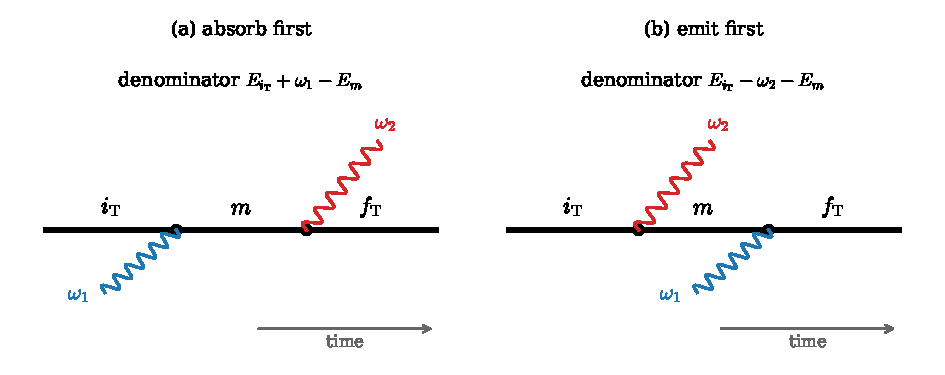
\includegraphics[width=\linewidth]{figures/ch02/fig2_4.pdf}
  \caption{The two time orderings of a second-order process in which a target goes from state $i_{\mathrm{T}}$ to state $f_{\mathrm{T}}$ while absorbing a quantum of energy $\omega_1$ and emitting one of energy $\omega_2$. Time runs to the right; the thick line is the target and the wavy lines are the quanta (absorbed from below, emitted upward). (a) Absorb first: the intermediate state is the target in $m$ with no quanta, of energy $E_m$. (b) Emit first: the target is in $m$ while both quanta are present, of energy $E_m + \omega_1 + \omega_2$. Each panel gives the energy denominator, the initial energy $E_{i_{\mathrm{T}}} + \omega_1$ minus the intermediate energy, with which its amplitude enters \cref{eq:2.4-orderings}.}
  \label{fig:2-orderings}
\end{figure}

Both orderings connect the same states, and their amplitudes add before squaring and can interfere. If $i_{\mathrm{T}}$ is the ground state of the target, $E_m \ge E_{i_{\mathrm{T}}}$ for every $m$, and the emit-first denominator $E_{i_{\mathrm{T}}} - \omega_2 - E_m$ is at most $-\omega_2$: it never vanishes, and this ordering is always off shell. The absorb-first denominator vanishes when $\omega_1 = E_m - E_{i_{\mathrm{T}}}$, that is, when quantum 1 alone could excite the target to a real state $m$. This is the resonance, and near it the absorb-first ordering dominates. Far from every resonance the two orderings are of similar size, and dropping one changes the rate by a factor of a few or more, as \cref{we:2-twophoton} shows. In silicon, with quantum 1 a photon and quantum 2 a phonon, \cref{eq:2.4-orderings} is the bracket of the theory of phonon-assisted absorption of Hall, Bardeen and Blatt~\cite{hall1954infrared}, which also includes phonon absorption in place of emission; Ref.~\cite[Eq.~(200)]{giustino2017electron} writes it in first-principles form. The photon-first term has the denominator of a direct, vertical transition at fixed crystal momentum, and the phonon-first term the denominator of an electron scattered by the phonon before the photon arrives. \Cref{sec:6.5} evaluates both. When the modes hold $n_1$ and $n_2$ quanta rather than one and zero, the matrix elements of $d_1$ and $d_2^\dagger$ bring factors $\sqrt{n_1}$ and $\sqrt{n_2 + 1}$, in both orderings alike; \cref{sec:2.5} averages them over thermal populations.

In a target with many electrons, $i_{\mathrm{T}}$, $m$ and $f_{\mathrm{T}}$ are the many-electron states of \cref{sec:2.3}, and the denominators are differences of total energies. For independent electrons they reduce to differences of orbital energies, because an operator that moves one electron from $\gamma'$ to $\gamma$ changes the total energy by $E_\gamma - E_{\gamma'}$, the frequency at which $c^\dagger_\gamma c_{\gamma'}$ oscillates in the interaction picture. If the photon moves an electron from an occupied valence orbital to an empty conduction orbital at the same crystal momentum, the absorb-first denominator is the photon energy minus that vertical transition energy, whatever the other electrons do. The Pauli principle changes the list of intermediate states. A state in which the moved electron would enter an occupied orbital does not exist. In its place there are orderings in which a different electron moves first and the electron moved by the photon then fills the hole it left, with the anticommutation sign of \cref{sec:2.3} attached to the amplitude. The single-particle picture of one electron passing through an intermediate band is a convenient way of organizing these terms, not a literal history, and \cref{sec:6.5} counts them for silicon.

\subsection{Resonance and finite width}

At resonance the absorb-first term of \cref{eq:2.4-orderings} is infinite, and the rate with it. Nothing in nature diverges here. The trouble is that \cref{eq:2.4-c2} lets the system stay in $m$ forever with unit probability, while a real excited state decays. Quantum 1 can take the target to $m$, and $m$ then empties into $f_{\mathrm{T}}$ by emitting quantum 2, or into any other state it is coupled to. We need the time dependence of a state that decays into a continuum, and this is the Wigner--Weisskopf problem~\cite{weisskopf1930berechnung}. A state that empties at rate $\varGamma_{\mathrm{w}}$ survives for a time of about $1/\varGamma_{\mathrm{w}}$, so its energy is defined only to within about $\varGamma_{\mathrm{w}}$, and a denominator that would vanish should instead saturate at a size of order $\varGamma_{\mathrm{w}}$.

Take a discrete state $|i\rangle$ coupled by a constant $H'$ to a continuum of states $|f\rangle$, with no other couplings, as in \cref{sec:2.1}. \Cref{app:D.3} solves the amplitude equations \cref{eq:2.1-exact} for this case without assuming that $c_i$ stays close to one. Under the condition that made the golden rule possible, $\varGamma_i \ll E_{\mathrm{w}}$, the memory of the continuum is short compared with the decay time. At times $t \gg 1/E_{\mathrm{w}}$ the amplitude of the initial state is then
\begin{equation}
  c_i(t) = \ee^{-(\varGamma_i/2 + \ii\Delta E_i)\,t}, \qquad
  \Delta E_i = \operatorname{PV}\sum_f\frac{|H'_{fi}|^2}{E_i - E_f} ,
  \label{eq:2.4-WW}
\end{equation}
where $\varGamma_i$ is the golden-rule rate \cref{eq:2.1-total} and $\operatorname{PV}$ denotes the principal value of the sum, made precise in the next subsection. The probability $|c_i|^2 = \ee^{-\varGamma_it}$ decays exponentially at the golden-rule rate, which justifies the statement of \cref{sec:2.1} that $\varGamma_i$ keeps its meaning beyond the first-order window (\cref{we:2-continuum}). The energy of the state is shifted by $\Delta E_i$, the second-order level shift of stationary perturbation theory, now with the principal value that a continuum requires; in \cref{we:2-continuum} the shift vanishes because the continuum is symmetric about resonance. The populations of the final states at late times trace out the line,
\begin{equation}
  |c_f(\infty)|^2 = \frac{|H'_{fi}|^2}{(E_f - E_i - \Delta E_i)^2 + \varGamma_i^2/4} ,
  \label{eq:2.4-lorentz}
\end{equation}
a Lorentzian of full width $\varGamma_i$ at half maximum, centered at the shifted energy. Summed over the continuum with density $\mathcal{D}_f$, it integrates to $\overline{|H'_{fi}|^2}\mathcal{D}_f\cdot 2\pi/\varGamma_i = 1$: the decaying state has gone somewhere, and the golden-rule rate fixes both how fast and how sharply in energy. The same shape describes the cross-section near a resonance in scattering, where it is called a Breit--Wigner line. \Cref{app:D.3} also states the limits of the exponential law. It fails at times shorter than $1/E_{\mathrm{w}}$, where the decay starts quadratically as in \cref{we:2-continuum}. It also fails after many lifetimes, where the edges of the continuum leave a slow power-law tail, by then far below any measurable level when $\varGamma_i \ll E_{\mathrm{w}}$.

Back to the intermediate state. Between $t_2$ and $t_1$ in \cref{eq:2.4-c2} the system evolves in $m$. \Cref{eq:2.4-WW} applied to $m$ replaces its free phase $\ee^{-\ii E_m(t_1 - t_2)}$ by $\ee^{-\ii(\tilde E_m - \ii\varGamma_{\mathrm{w}}/2)(t_1 - t_2)}$, where $\tilde E_m = E_m + \Delta E_m$ is the shifted energy and $\varGamma_{\mathrm{w}}$ the total decay rate of $m$, summed over all of its decay channels. The inner time integral then converges without any switching and gives
\begin{equation}
  \frac{1}{E_i - E_m + \ii0^+} \;\longrightarrow\; \frac{1}{E_i - \tilde E_m + \ii\varGamma_{\mathrm{w}}/2} .
  \label{eq:2.4-width}
\end{equation}
The infinitesimal becomes a finite width, and at resonance the amplitude is large, $-2\ii/\varGamma_{\mathrm{w}}$ in place of the denominator, but finite. In the language of the Dyson series, \cref{eq:2.4-width} keeps, from every order, the repeated emission and reabsorption that happen while the system sits in $m$. These are the terms that grow near resonance, and summing them is consistent under the same condition as before, $\varGamma_{\mathrm{w}}$ small compared with the energy over which the decay continuum of $m$ changes. Off resonance, with $|E_i - \tilde E_m| \gg \varGamma_{\mathrm{w}}$, the width is a small correction and the shift is usually absorbed in the measured energy $\tilde E_m$. From now on we write $E_m$ for the shifted energy. In a solid the width of an excited electron comes from the emission of phonons and from scattering with other electrons, and it depends on how far above the band edge the electron sits; \cref{sec:6.3} computes the phonon part. For the off-resonant denominators that dominate below a direct gap, an infinitesimal $\ii0^+$ is enough.

\subsection{Principal value and finite part}

An energy denominator regularized by a width, $1/(x + \ii\varGamma_{\mathrm{w}}/2)$ with $x = E_i - E_m$, has a real and an imaginary part,
\begin{equation*}
  \frac{1}{x + \ii\varGamma_{\mathrm{w}}/2} = \frac{x}{x^2 + \varGamma_{\mathrm{w}}^2/4} - \ii\,\frac{\varGamma_{\mathrm{w}}/2}{x^2 + \varGamma_{\mathrm{w}}^2/4} ,
\end{equation*}
drawn in \cref{fig:2-denominator}(a). The real part equals $1/x$ for $|x| \gg \varGamma_{\mathrm{w}}$ and turns over smoothly through zero inside $|x| < \varGamma_{\mathrm{w}}/2$, with extrema $\pm1/\varGamma_{\mathrm{w}}$. The imaginary part is a Lorentzian of area $\pi$ and depth $2/\varGamma_{\mathrm{w}}$. As $\varGamma_{\mathrm{w}} \to 0$ the Lorentzian becomes $\pi\delta(x)$. The real part, integrated against a smooth function $w(x)$, becomes $\int\dd x\,x[w(x) - w(0)]/(x^2 + \varGamma_{\mathrm{w}}^2/4)$, since $x/(x^2 + \varGamma_{\mathrm{w}}^2/4)$ is odd, and this tends to $\int\dd x\,[w(x) - w(0)]/x$. That is the principal value of $\int\dd x\,w(x)/x$: the integral with a symmetric interval $(-x_{\mathrm{c}}, x_{\mathrm{c}})$ cut out around the pole, in the limit $x_{\mathrm{c}} \to 0$, in which the divergences on the two sides cancel. Together these limits are the Sokhotski--Plemelj formula,
\begin{equation}
  \frac{1}{x + \ii0^+} = \operatorname{PV}\frac{1}{x} - \ii\pi\,\delta(x) ,
  \label{eq:2.4-SP}
\end{equation}
which \cref{app:C.4} proves for the general case. Applied to a second-order amplitude, it splits the sum over intermediate states into two parts with different physics. The principal-value part collects the off-shell intermediate states, and it is real: it shifts energies, as $\Delta E_i$ does in \cref{eq:2.4-WW}, and it produces the dispersive effects of a medium. The delta part picks out the on-shell intermediate states, those with $E_m = E_i$; it is imaginary and produces the decay. \Cref{eq:2.4-WW} is the example: the self-coupling of $i$ through the continuum, $\sum_f|H'_{fi}|^2/(E_i - E_f + \ii0^+)$, is $\Delta E_i - \ii\varGamma_i/2$ by \cref{eq:2.4-SP}. The same statement can be read off the T-matrix. The forward element at second order, $T_{ii} = \sum_f|H'_{fi}|^2/(E_i - E_f + \ii0^+)$, has imaginary part $-\pi\sum_f|H'_{fi}|^2\delta(E_f - E_i) = -\varGamma_i/2$. The total decay rate of a state is $-2\Imag T_{ii}$, the lowest-order form of the optical theorem, which follows in general from the unitarity of the evolution: the probability that leaves $i$ is the probability that arrives in all the states $f$.

The principal-value part has a familiar instance in light scattering. Let quanta 1 and 2 be photons of the same frequency, so that the target absorbs one photon and emits another and returns to $f_{\mathrm{T}} = i_{\mathrm{T}}$. \Cref{eq:2.4-orderings} is then the amplitude of elastic (Rayleigh) scattering, and below every resonance both orderings are off shell and real. Summed over intermediate states, the two orderings combine into $\sum_m 2(E_m - E_{i_{\mathrm{T}}})|\langle m|\op{O}|i_{\mathrm{T}}\rangle|^2/[\omega^2 - (E_m - E_{i_{\mathrm{T}}})^2]$, for a Hermitian $\op{O}$. For a dipole coupling, $\op{O}$ is the field amplitude times the dipole operator along the field, and the sum is minus the dynamic polarizability of the target, whose denominators are $(E_m - E_{i_{\mathrm{T}}})^2 - \omega^2$, times the square of the field amplitude. Its imaginary part, which appears once a width or a continuum puts the absorb-first denominator on shell, is absorption. The dielectric function of \cref{sec:4.4} has the same structure, with a real part made of off-shell transitions and an imaginary part made of on-shell ones.

\begin{figure}[tbp]
  \centering
  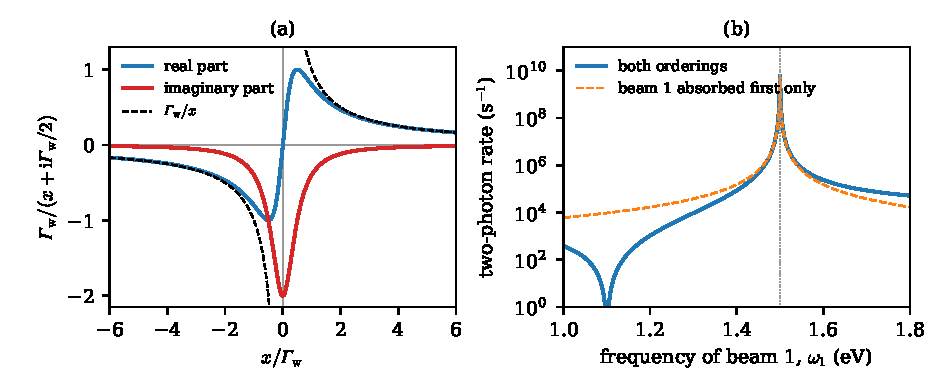
\includegraphics[width=\linewidth]{figures/ch02/fig2_5.pdf}
  \caption{(a) Real and imaginary parts of an energy denominator regularized by a width, $1/(x + \ii\varGamma_{\mathrm{w}}/2)$, multiplied by $\varGamma_{\mathrm{w}}$ and plotted against $x/\varGamma_{\mathrm{w}}$, where $x$ is the initial energy minus the intermediate energy. Dashed: $\varGamma_{\mathrm{w}}/x$, to which the real part tends for $|x| \gg \varGamma_{\mathrm{w}}$. As $\varGamma_{\mathrm{w}} \to 0$ the real part becomes the principal value of $1/x$ and the imaginary part $-\pi\delta(x)$. (b) Rate of two-photon absorption in the three-level model of \cref{we:2-twophoton}, against the frequency $\omega_1$ of beam 1 at fixed $\omega_2 = \SI{1.90}{eV}$, for the channel with final energy $\omega_1 + \omega_2$. The model has a ground level $i_{\mathrm{T}}$, an intermediate level $m$ at \SI{1.50}{eV} with total width $\varGamma_{\mathrm{w}} = \SI{1}{meV}$, and a flat band of final states above \SI{3.20}{eV}. Either beam drives $i_{\mathrm{T}} \to m$ with matrix element \SI{0.1}{meV}, and beam 2 empties a real level $m$ into the band at the rate \SI{0.1}{meV}. Solid: both time orderings. Dashed: the ordering in which beam 1 is absorbed first, alone. The peak at $\omega_1 = \SI{1.50}{eV}$ is the resonance with $m$; the zero at \SI{1.10}{eV} is destructive interference between the two orderings.}
  \label{fig:2-denominator}
\end{figure}

The rate needs the squared modulus, and near resonance this brings a double pole. With $|E_i - E_m + \ii\varGamma_{\mathrm{w}}/2|^{-2} = 1/(x^2 + \varGamma_{\mathrm{w}}^2/4)$, the limit $\varGamma_{\mathrm{w}} \to 0$ cannot be taken in \cref{eq:2.4-SP}: the square of $\ii\pi\delta(x)$ has no meaning, as the square of the momentum delta function had none in \cref{sec:2.1}. The function $1/x^2$ has no principal value either. Its singularity is even, the divergences on the two sides add instead of cancelling, and $\int_{|x| > x_{\mathrm{c}}}\dd x/x^2 = 2/x_{\mathrm{c}}$. The Hadamard finite part removes exactly this divergence:
\begin{equation}
  \operatorname{fp}\!\int\dd x\,\frac{w(x)}{x^2}
  = \lim_{x_{\mathrm{c}}\to0}\left[\int_{|x|>x_{\mathrm{c}}}\dd x\,\frac{w(x)}{x^2} - \frac{2w(0)}{x_{\mathrm{c}}}\right]
  = \int_0^\infty\dd x\,\frac{w(x) + w(-x) - 2w(0)}{x^2} .
  \label{eq:2.4-fp}
\end{equation}
The integrand on the right is finite at $x = 0$, where it tends to $w''(0)$. With it, the Lorentzian of the rate splits as follows. Write $\int\dd x\,w(x)/(x^2 + \varGamma_{\mathrm{w}}^2/4)$ as $w(0)\int\dd x/(x^2 + \varGamma_{\mathrm{w}}^2/4) = 2\pi w(0)/\varGamma_{\mathrm{w}}$ plus $\int\dd x\,[w(x) - w(0)]/(x^2 + \varGamma_{\mathrm{w}}^2/4)$. The remainder tends to the finite part as $\varGamma_{\mathrm{w}} \to 0$, since its integrand is integrable at $x = 0$. Its difference from the limit is $-(\varGamma_{\mathrm{w}}^2/4)\int\dd x\,[w(x) - w(0)]/[x^2(x^2 + \varGamma_{\mathrm{w}}^2/4)]$, which is dominated by $|x| \lesssim \varGamma_{\mathrm{w}}$. There the odd part of $w(x) - w(0)$ drops out and the even part is $w''(0)x^2/2$, and the difference is $-(\varGamma_{\mathrm{w}}^2/8)\,w''(0)\cdot 2\pi/\varGamma_{\mathrm{w}} = -\pi\varGamma_{\mathrm{w}}w''(0)/4$. In the sense of distributions,
\begin{equation}
  \frac{1}{x^2 + \varGamma_{\mathrm{w}}^2/4} = \frac{2\pi}{\varGamma_{\mathrm{w}}}\,\delta(x) + \operatorname{fp}\frac{1}{x^2} - \frac{\pi\varGamma_{\mathrm{w}}}{4}\,\delta''(x) + O(\varGamma_{\mathrm{w}}^2) .
  \label{eq:2.4-split}
\end{equation}
For a function $w$ that varies on an energy scale $\Delta_{\mathrm{w}}$, the delta term is of size $w/\varGamma_{\mathrm{w}}$, the finite part of size $w/\Delta_{\mathrm{w}}$, and the correction a fraction $(\varGamma_{\mathrm{w}}/\Delta_{\mathrm{w}})^2$ of the delta term. \Cref{app:C.4} collects these definitions.

The two terms of \cref{eq:2.4-split} are the on-shell and the off-shell parts of a resonant second-order rate, and the on-shell part has a direct interpretation. Inserted in \cref{eq:2.4-golden2}, the delta term of the absorb-first ordering is the first-order golden-rule rate $2\pi|\langle m|\op{O}_a|i_{\mathrm{T}}\rangle|^2\delta(E_{i_{\mathrm{T}}} + \omega_1 - E_m)$, at which quantum 1 creates a real state $m$, multiplied by $2\pi|\langle f_{\mathrm{T}}|\op{O}_b^\dagger|m\rangle|^2\delta(E_f - E_i)/\varGamma_{\mathrm{w}}$. Summed over final states, this factor is the fraction of the decays of $m$ that end in $f_{\mathrm{T}}$. The on-shell part is a cascade of two first-order processes, the excitation of $m$ and its decay into $f_{\mathrm{T}}$, the decay weighted by its branching ratio. The finite part is what remains of the genuinely second-order process, the virtual passage through $m$. It is not positive: against a function $w$ peaked at $x = 0$ with width $\Delta_{\mathrm{w}}$, \cref{eq:2.4-fp} is about $-w(0)/\Delta_{\mathrm{w}}$, because $w(x) - w(0) < 0$ near the peak. Only the sum of the two parts is a rate. This is the reason for care in any calculation that counts the cascade separately, as two first-order events, and also includes a second-order rate: the delta part of the second-order rate is then counted twice. The resonant denominators of phonon-assisted absorption return in \cref{sec:6.5}, where the electron in the intermediate state becomes real once the photon energy exceeds the direct gap.

\subsection{Forbidden first-order transitions}

Since each order costs a factor $|H'|/|E_i - E_m|$, a second-order process competes with a first-order one only when the first-order rate vanishes, by a selection rule or by kinematics.

If a symmetry of the target makes $\langle f|H'|i\rangle = 0$ for every final state at the right energy, the leading amplitude is the second-order sum, which involves different matrix elements. The classic case is parity. The electric-dipole operator is odd, and a single photon cannot connect two states of the same parity. Two photons can, through intermediate states of the opposite parity. The metastable $2s$ level of hydrogen decays by emitting two photons, and two-photon absorption spectroscopy reaches levels that one photon cannot. Spin, angular momentum and the symmetries of a crystal impose rules of the same kind.

Kinematics closes the first-order channel when no final state conserves both energy and momentum. The opening example is of this type. A vertical transition at fixed crystal momentum needs an energy well above the \SI{1.12}{eV} gap at \SI{300}{K}, because the conduction-band minimum and the valence-band maximum sit at different crystal momenta (\cref{sec:3.3}). Below that energy the first-order rate is zero, and phonon-assisted absorption, with the amplitude \cref{eq:2.4-orderings}, is the leading process. The phonon costs or supplies tens of meV of energy~\cite[Table~I]{kahn2022searches}, but it can carry any crystal momentum in the zone. The same holds for absorbed dark matter. A boson of mass $m_\phi$ is absorbed with momentum $m_\phi v \approx 10^{-3}m_\phi$ (\cref{sec:2.1}), even smaller compared to its energy than a photon's, and in an indirect-gap material its absorption between the indirect and the direct gap is a second-order process (\cref{chap:8}). Dark-matter scattering is different. The momentum transfer is typically $q \sim q_0 = \alpha m_e = \SI{3.73}{keV}$, which is \SI{1.89}{\angstrom^{-1}}, larger than $2\pi/a$, so scattering reaches the indirect transitions at first order. At small momentum transfer, however, scattering runs into the same obstacle as a photon, and there the simultaneous emission of a phonon, the dark-matter analogue of phonon-assisted absorption, takes over~\cite[Sect.~VI]{kahn2022searches}. The Migdal effect is a process of the same structure, with a nuclear recoil in place of the phonon (\cref{sec:12.2}).

In each case the size of the second-order rate relative to a first-order one is set by $|H_2|^2/(E_i - E_m)^2$, with $H_2$ the coupling that the second-order route adds and $E_i - E_m$ the off-shell distance of the intermediate state. \Cref{sec:8.5} names this ratio for the electron--phonon coupling and uses it to organize the expansion.

When the first-order amplitude does not vanish, second order is a correction to it, and it enters the rate through the cross term $2\Real(A_1A_2^*)$, at relative order $|H'|/|E_i - E_m|$ rather than its square. Corrections of this kind are part of the target response when $H_2$ is internal to the target. They are already contained in an exact treatment of the target's states, such as the band structure with its phonon renormalization (\cref{sec:6.3}), and are not added again as second-order rates. A second-order rate is a separate channel only when it leads to a final state that first order cannot reach, such as a state with one more phonon.

\begin{workedexample}{Two-photon absorption in a three-level system}\label{we:2-twophoton}
A target has a ground level $a$ at zero energy, an intermediate level $m$ at $E_m = \SI{1.50}{eV}$, and a flat band of final states $f_{\mathrm{T}}$ above \SI{3.20}{eV}, with density of states $\mathcal{D}_{f_{\mathrm{T}}}$. Two light beams of frequencies $\omega_1$ and $\omega_2$ couple to the target through the same operator $\op{O}$ (equal polarization and intensity); \cref{sec:2.1} showed that a classical beam acts like a quantized mode holding many photons, and we use the language of \cref{eq:2.4-orderings}. Here, however, both photons are absorbed, so the ordering that absorbs $\omega_2$ first has the denominator $E_{i_{\mathrm{T}}} + \omega_2 - E_m$, with $+\omega_2$ in place of the $-\omega_2$ of emission in \cref{eq:2.4-orderings}. We fix $\omega_2 = \SI{1.90}{eV}$ and tune $\omega_1$ near \SI{1.50}{eV}. Neither photon alone reaches the band, and neither do two photons of beam 1 for $\omega_1 < \SI{1.60}{eV}$: the first-order rate is kinematically zero. The pair $\omega_1 + \omega_2 \approx \SI{3.40}{eV}$ reaches the band. Two photons of beam 2 reach it too, at \SI{3.80}{eV}; that final state differs from ours and does not interfere, and we follow the channel with final energy $\omega_1 + \omega_2$. The model numbers are $|\langle m|\op{O}|i_{\mathrm{T}}\rangle| = \SI{0.1}{meV}$, a rate $\varGamma_{m\to f_{\mathrm{T}}} = 2\pi\overline{|\langle f_{\mathrm{T}}|\op{O}|m\rangle|^2}\,\mathcal{D}_{f_{\mathrm{T}}} = \SI{0.1}{meV}$ at which beam 2 empties a real level $m$ into the band (beam 1 cannot, since $E_m + \omega_1 < \SI{3.20}{eV}$), and a total width $\varGamma_{\mathrm{w}} = \SI{1}{meV}$ of $m$, which includes $\varGamma_{m\to f_{\mathrm{T}}}$ and all other decays.

Both orderings absorb one photon from each beam. Absorbing $\omega_1$ first leaves the target in $m$ with photon $\omega_2$ still present, and the denominator is $\delta_1 = E_{i_{\mathrm{T}}} + \omega_1 - E_m = \omega_1 - \SI{1.50}{eV}$; absorbing $\omega_2$ first leads to $\delta_2 = \omega_2 - \SI{1.50}{eV} = \SI{0.40}{eV}$. With \cref{eq:2.4-width},
\begin{equation*}
  T_{fi} = \langle f_{\mathrm{T}}|\op{O}|m\rangle\langle m|\op{O}|i_{\mathrm{T}}\rangle\,\mathcal{A}(\omega_1), \qquad
  \mathcal{A}(\omega_1) = \frac{1}{\delta_1 + \ii\varGamma_{\mathrm{w}}/2} + \frac{1}{\delta_2 + \ii\varGamma_{\mathrm{w}}/2} ,
\end{equation*}
and summing \cref{eq:2.4-golden2} over the flat band gives $\varGamma_{i_{\mathrm{T}}\to f_{\mathrm{T}}} = \varGamma_{m\to f_{\mathrm{T}}}\,|\langle m|\op{O}|i_{\mathrm{T}}\rangle|^2\,|\mathcal{A}|^2$. \Cref{fig:2-denominator}(b) plots the rate against $\omega_1$.

Off resonance, at $\omega_1 = \SI{1.20}{eV}$, $\delta_1 = \SI{-0.30}{eV}$ and $\mathcal{A} = -3.33 + 2.50 = \SI{-0.833}{eV^{-1}}$. The two orderings have denominators of opposite sign and interfere destructively. Beam 1 is below the resonance of $m$ and beam 2 above it, and the virtual excitation of $m$ follows the two beams with opposite phases, as a driven oscillator follows a force below and above its natural frequency. The rate is $\SI{6.9e-13}{eV}$, or \SI{1.1e3}{s^{-1}}; keeping the absorb-$\omega_1$-first ordering alone would overestimate it by a factor of 16. At $\omega_1 = \SI{1.10}{eV}$ the two denominators are equal and opposite, and the rate vanishes up to terms of relative order $(\varGamma_{\mathrm{w}}/\delta_2)^2$.

On resonance, at $\omega_1 = \SI{1.50}{eV}$, the first denominator is $-2\ii/\varGamma_{\mathrm{w}}$ and $|\mathcal{A}|^2 = \SI{4.0e6}{eV^{-2}}$, so $\varGamma_{i_{\mathrm{T}}\to f_{\mathrm{T}}} = \SI{4.0e-6}{eV} = \SI{6.1e9}{s^{-1}}$, larger than the off-resonant rate by $5.8\times10^6$. The cascade picture reproduces this number. On resonance, beam 1 excites $m$ at the first-order rate $2\pi|\langle m|\op{O}|i_{\mathrm{T}}\rangle|^2$ times the peak $2/(\pi\varGamma_{\mathrm{w}})$ of the Lorentzian of $m$, that is $4|\langle m|\op{O}|i_{\mathrm{T}}\rangle|^2/\varGamma_{\mathrm{w}} = \SI{4.0e-5}{eV}$; a fraction $\varGamma_{m\to f_{\mathrm{T}}}/\varGamma_{\mathrm{w}} = 0.10$ of the excited levels end in the band. The product agrees with the second-order rate to five parts in $10^6$, the contribution of the off-resonant ordering. Perturbation theory holds, since the probability of finding the target in $m$ on resonance is $|\langle m|\op{O}|i_{\mathrm{T}}\rangle|^2/(\varGamma_{\mathrm{w}}/2)^2 = 0.04$.

A broadband beam 1 tests \cref{eq:2.4-split}. Let its spectrum be a Gaussian of rms width \SI{10}{meV} in $\delta_1$, normalized to one; the measured rate is $|\mathcal{A}|^2$ averaged over it. Centered on resonance, the exact average is \SI{2.410e5}{eV^{-2}}. The delta term of \cref{eq:2.4-split} is $(2\pi/\varGamma_{\mathrm{w}})$ times the spectral density at resonance, \SI{2.507e5}{eV^{-2}}, an overestimate by \SI{4.0}{\percent}. The finite part, $-1/(\SI{10}{meV})^2 = \SI{-1.00e4}{eV^{-2}}$ for a centered Gaussian, is negative, as it must be for a spectrum peaked at the pole. Delta and finite part together are within \SI{0.13}{\percent} of the exact value, and the remainder matches the term $-\pi\varGamma_{\mathrm{w}}w''(0)/4$. Centered \SI{30}{meV} away from resonance, the delta term is \SI{2785}{eV^{-2}}, the finite part \SI{+1795}{eV^{-2}}, now positive, the principal-value cross term between the two orderings \SI{197}{eV^{-2}}, and the off-resonant ordering \SI{6}{eV^{-2}}. Their sum is within \SI{0.6}{\percent} of the exact average, \SI{4753}{eV^{-2}}, while the delta term alone misses it by \SI{41}{\percent}. The cascade accounts for nearly the whole rate only when the spectrum sits on the resonance and is broad compared with $\varGamma_{\mathrm{w}}$. Even then the finite part corrects it by about $\varGamma_{\mathrm{w}}$ divided by the spectral width. Away from resonance, the finite part and the cross term between the orderings are as large as the cascade itself.
\end{workedexample}

\section{Thermal states and detailed balance}\label{sec:2.5}

At \SI{300}{K} each optical phonon mode of silicon at the zone center, at \SI{64}{meV}, holds on average 0.09 quanta; at the \SI{4}{K} of a liquid-helium cryostat it holds $10^{-81}$. A crystal at a finite temperature is not in an eigenstate of its Hamiltonian, as the rates of \cref{sec:2.1,sec:2.2} assumed, but in a statistical mixture of them, and an excited component of the mixture can give its energy to the dark matter. This is the negative $\omega$ that \cref{sec:1.3} allowed. At zero temperature the same occupation numbers produce the filled Fermi sea of a free electron gas, whose Fermi momentum and density of states \cref{chap:4} uses throughout. We follow Refs.~\cite{landau1980statistical} and \cite[Chap.~1]{bruus2004many} for the ensembles and Ref.~\cite[Chap.~2]{ashcroft1976solid} for the free electron gas.

\subsection{Gibbs state}

A mixture that holds the eigenstate $|i\rangle$ with probability $p_i$ is described by the density matrix
\begin{equation}
  \op{\varrho} = \sum_i p_i\,|i\rangle\langle i|, \qquad \langle\op{A}\rangle = \Tr\bigl(\op{\varrho}\,\op{A}\bigr) = \sum_i p_i\,\langle i|\op{A}|i\rangle ,
  \label{eq:2.5-rho}
\end{equation}
with $\sum_ip_i = 1$; the thermal average $\langle\op{A}\rangle$ is the quantum expectation value averaged over the mixture. A target in equilibrium with a bath at temperature $T$ has the Gibbs weights
\begin{equation}
  p_i = \frac{\ee^{-\beta E_i}}{\mathcal{Z}}, \qquad \mathcal{Z} = \sum_i\ee^{-\beta E_i} = \Tr\,\ee^{-\beta H}, \qquad \beta = \frac{1}{T},
  \label{eq:2.5-gibbs}
\end{equation}
so that $\op{\varrho} = \ee^{-\beta H}/\mathcal{Z}$, with $\mathcal{Z}$ the partition function. In natural units temperature is an energy, $\SI{1}{K} = \SI{86.17}{\micro eV}$, and a detector at \SI{10}{mK} has $T = \SI{0.86}{\micro eV}$.

Since the Gibbs state is a function of $H$, it commutes with $H$, and its time evolution $\op{\varrho}(t) = \ee^{-\ii Ht}\op{\varrho}\,\ee^{\ii Ht}$ leaves it unchanged: it is a stationary state, and every thermal average is independent of time. A correlation $\langle\op{A}(t)\op{B}(t')\rangle$ of Heisenberg operators $\op{A}(t) = \ee^{\ii Ht}\op{A}\,\ee^{-\ii Ht}$ depends only on $t - t'$, which is what makes its Fourier transform in time a function of one frequency (\cref{sec:4.1}). Note that stationarity does not need the Gibbs form; any $\op{\varrho}$ diagonal in the energy basis has it. Thermal equilibrium fixes the weights.

Particles can also be exchanged with a reservoir, or we may prefer to fix their mean number instead of the exact one. The grand-canonical state then replaces $H$ by $H - \mu_{\mathrm{ch}}\op{N}$, with $\op{N}$ the particle-number operator and $\mu_{\mathrm{ch}}$ the chemical potential:
\begin{equation}
  \op{\varrho} = \frac{\ee^{-\beta(H - \mu_{\mathrm{ch}}\op{N})}}{\mathcal{Z}}, \qquad p_i = \frac{\ee^{-\beta(E_i - \mu_{\mathrm{ch}}N_i)}}{\mathcal{Z}} .
  \label{eq:2.5-grand}
\end{equation}
The value of $\mu_{\mathrm{ch}}$ is fixed by $\langle\op{N}\rangle = N$. A detector holds a fixed number of electrons, and the canonical state is the physical one. However, the two ensembles differ in a macroscopic body by fluctuations of relative size $N^{-1/2}$, and the grand-canonical state is much easier to use, since for independent particles it factorizes into one factor per single-particle state (\cref{eq:2.5-nF} below).

\subsection{Thermal golden rule}

The probability of finding the system in $|f\rangle$ at time $t$ is linear in the initial density matrix. With $U(t)$ the evolution operator,
\begin{equation*}
  \langle f|U(t)\,\op{\varrho}\,U(t)^\dagger|f\rangle = \sum_ip_i\,|\langle f|U(t)|i\rangle|^2 = \sum_ip_i\,P_{i\to f}(t) .
\end{equation*}
Different initial states do not interfere, because $\op{\varrho}$ has no off-diagonal elements between them. Each $P_{i\to f}$ grows at its golden-rule rate (\cref{eq:2.1-golden}), and the rate out of the thermal state is the weighted sum
\begin{equation}
  \varGamma = \sum_ip_i\sum_f\varGamma_{i\to f} .
  \label{eq:2.5-thermalrate}
\end{equation}
For dark-matter scattering the initial state is the product of the thermal target and a dark-matter plane wave of momentum $\vect{p}$, and the final state has the target in $|f\rangle$ and the dark matter at $\vect{p} - \vect{q}$. The interaction between these two dark-matter states is $\tilde V(\vect{q})\,n_e(\vect{q})/\Vol$ (\cref{eq:2.3-nq}), and energy conservation, with the dark-matter energies written out, is $\delta(\omega_{\vect{q}} - E_f + E_i)$, where $\omega_{\vect{q}}$ is the energy lost by the dark matter (\cref{eq:1.3-omegaq}). Summing \cref{eq:2.5-thermalrate} over the final momenta,
\begin{equation*}
  \varGamma = \sum_{\vect{q}}\frac{2\pi}{\Vol^2}\,|\tilde V(\vect{q})|^2\,\mathcal{S}_{n_e(\vect{q})}(\omega_{\vect{q}}),
\end{equation*}
where all the target physics sits in the transition sum of an operator $\op{O}$,
\begin{equation}
  \mathcal{S}_O(\omega) = \sum_{i,f}p_i\,|\langle f|\op{O}|i\rangle|^2\,\delta(\omega - E_f + E_i) .
  \label{eq:2.5-transum}
\end{equation}
It counts the transitions that $\op{O}$ drives from the thermal state, weighted by their probability, at each energy $\omega$ given to the target. The same object is the Fourier transform of a thermal correlation function. Inserting a complete set of states between the operators of $\langle\op{O}^\dagger(t)\op{O}(0)\rangle$, each term oscillates as $\ee^{\ii(E_i - E_f)t}$, and the time integral turns it into a delta function:
\begin{equation}
  \int_{-\infty}^{\infty}\dd t\;\ee^{\ii\omega t}\,\langle\op{O}^\dagger(t)\,\op{O}(0)\rangle = 2\pi\,\mathcal{S}_O(\omega) .
  \label{eq:2.5-corr}
\end{equation}
The rate measures how the fluctuations of $\op{O}$ in the equilibrium state are correlated in time, the viewpoint that \cref{sec:4.2} develops. With \cref{eq:2.1-box} for the sum over $\vect{q}$,
\begin{keyresult}[Thermal golden rule]
\begin{equation}
  \varGamma = \int\frac{\dd^3q}{(2\pi)^3}\,\underbrace{|\tilde V(\vect{q})|^2}_{\text{coupling}}\,\underbrace{S(\vect{q},\omega_{\vect{q}})}_{\text{target}}, \qquad
  S(\vect{q},\omega) = \frac{2\pi}{\Vol}\,\mathcal{S}_{n_e(\vect{q})}(\omega) .
  \label{eq:2.5-golden}
\end{equation}
$\varGamma$ is the scattering rate of one dark-matter particle of momentum $\vect{p}$ in a box of volume $\Vol$ filled by the target, which is in thermal equilibrium at temperature $T$.
\end{keyresult}
The function $S(\vect{q},\omega)$ is the dynamic structure factor of the electron density (\cref{eq:A.7-S})~\cite[Eq.~(4)]{knapen2021dark}; that reference writes the density at $-\vect{k}$ where we write $n_e(\vect{q})$ (\cref{app:A.7}); \cref{sec:4.2} develops it. The volume drops out as it should. The transition sum is extensive, since a target twice as large offers twice as many transitions, and $S$ is intensive. The rate of one dark-matter particle, present with density $1/\Vol$ in a target of volume $\Vol$, is then independent of $\Vol$.

The rate assembled in \cref{sec:1.5} now follows. For a target whose response depends only on $q = |\vect{q}|$, we write $S(q,\omega_{\vect{q}}) = \int\dd\omega\,S(q,\omega)\,\delta(\omega - \omega_{\vect{q}})$. The average of the delta function over the direction of $\vect{q}$ and over the halo is $\eta(\vmin)/2q$ (\cref{sec:1.3}; \cref{eq:2.2-spectrum}), and the measure becomes $\int\dd^3q/(2\pi)^3\,(2q)^{-1} = \int q\,\dd q/(2\pi)^2$. Multiplying by the number density $\rho_\chi/m_\chi$ of dark matter, dividing by the target mass density $\rho_T$ and inserting $|\tilde V|^2 = \pi\sigmae\FDM^2/\mu_{\chi e}^2$ (\cref{eq:1.4-Vsq}) reproduces \cref{eq:1.5-rate} term by term. Unlike the version of \cref{sec:1.5}, the derivation holds at any temperature, with the thermal weights inside $S$, and its integral over $\omega$ runs over negative values too.

\subsection{Detailed balance}

Negative $\omega$ means that the target gives energy to the dark matter. The weight of such transitions is tied to the weight of the reverse ones by relabeling the sum. Write the transition sum of $\op{O}^\dagger$ at $-\omega$ and exchange the names of the summed states $i$ and $f$:
\begin{equation*}
  \mathcal{S}_{O^\dagger}(-\omega) = \sum_{i,f}p_i\,|\langle f|\op{O}^\dagger|i\rangle|^2\,\delta(-\omega - E_f + E_i)
  = \sum_{i,f}p_f\,|\langle i|\op{O}^\dagger|f\rangle|^2\,\delta(\omega - E_f + E_i) .
\end{equation*}
Since $|\langle i|\op{O}^\dagger|f\rangle| = |\langle f|\op{O}|i\rangle|$, the identity of \cref{sec:2.1}, the matrix elements are those of $\mathcal{S}_O(\omega)$. The weights differ: the delta function sets $E_f = E_i + \omega$, where $p_f = p_i\,\ee^{-\beta\omega}$. Hence
\begin{keyresult}[Detailed balance]
\begin{equation}
  \mathcal{S}_{O^\dagger}(-\omega) = \ee^{-\beta\omega}\,\mathcal{S}_O(\omega) .
  \label{eq:2.5-db}
\end{equation}
For the electron density, $n_e(\vect{q})^\dagger = n_e(-\vect{q})$, and $S(-\vect{q},-\omega) = \ee^{-\beta\omega}S(\vect{q},\omega)$. For a target with inversion or time-reversal symmetry, $S(\vect{q},-\omega) = \ee^{-\beta\omega}S(\vect{q},\omega)$. The density form is the diagonal element of \cref{eq:A.7-DB}.
\end{keyresult}
In the grand-canonical state the weights carry $-\mu_{\mathrm{ch}}N$ as well, and the step $p_f = p_i\ee^{-\beta\omega}$ needs $N_f = N_i$. It holds for every operator that conserves particle number, such as $n_e(\vect{q})$; an operator that adds $\Delta N$ particles acquires the factor $\ee^{-\beta(\omega - \mu_{\mathrm{ch}}\Delta N)}$ instead. The symmetric form uses $S(-\vect{q},\omega) = S(\vect{q},\omega)$, which inversion or time reversal guarantees (\cref{app:A.4}); silicon has both.

Detailed balance holds for every target in equilibrium, whatever its interactions, because the argument used only the Gibbs weights. In a two-level system with splitting $\Delta_{\mathrm{tl}}$, driven by a Hermitian $\op{O}$ with matrix element $O_{10} = \langle 1|\op{O}|0\rangle$, the transition sum is
\begin{equation*}
  \mathcal{S}_O(\omega) = |O_{10}|^2\bigl[p_0\,\delta(\omega - \Delta_{\mathrm{tl}}) + p_1\,\delta(\omega + \Delta_{\mathrm{tl}})\bigr], \qquad \frac{p_1}{p_0} = \ee^{-\beta\Delta_{\mathrm{tl}}} .
\end{equation*}
The upward transition, at $\omega = +\Delta_{\mathrm{tl}}$, starts from the ground state; the downward one, at $\omega = -\Delta_{\mathrm{tl}}$, starts from the excited state and carries its population (\cref{fig:2-twolevel}). At $T = \Delta_{\mathrm{tl}}/2$ the weights are 0.881 and 0.119. At $T = 0$ the downward weight vanishes and $\omega \ge 0$. As $T \to \infty$ both tend to $\tfrac12$, but the upward weight never falls below the downward one: a thermal target always absorbs more often than it emits, by the factor $\ee^{\beta\omega}$.

\begin{figure}[tbp]
  \centering
  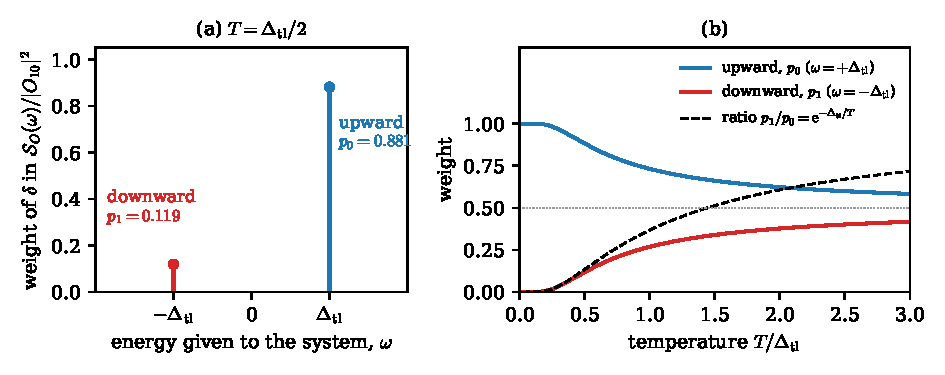
\includegraphics[width=\linewidth]{figures/ch02/fig2_6.pdf}
  \caption{Upward and downward transitions of a two-level system with splitting $\Delta_{\mathrm{tl}}$ in thermal equilibrium at temperature $T$, driven by a Hermitian operator $\op{O}$ with matrix element $O_{10}$. (a) At $T = \Delta_{\mathrm{tl}}/2$ the transition sum $\mathcal{S}_O(\omega)$ consists of two delta functions, drawn as stems with their weights in units of $|O_{10}|^2$. Upward, at energy $\omega = +\Delta_{\mathrm{tl}}$ given to the system, with the ground-state population $p_0 = 0.881$; downward, at $\omega = -\Delta_{\mathrm{tl}}$, with the excited-state population $p_1 = 0.119$. (b) The two weights against $T/\Delta_{\mathrm{tl}}$, and their ratio $p_1/p_0 = \ee^{-\Delta_{\mathrm{tl}}/T}$ (detailed balance). The weights approach $\tfrac12$ (dotted line) from either side as $T$ grows and never cross.}
  \label{fig:2-twolevel}
\end{figure}

The negative-$\omega$ part of the rate is suppressed by the Boltzmann factor of the excitation it removes, $\ee^{-\beta|\omega|}$ relative to the positive-$\omega$ part at the same $|\omega|$. For a \SI{1}{meV} acoustic phonon at \SI{1}{K}, $\beta\omega = 11.6$ and the factor is $9\times10^{-6}$; \cref{app:A.4} gives the case of an electronic gap. Note that such an event deposits no energy in the detector. The target loses energy to the dark matter, and a calorimeter or a charge readout registers nothing. Such transitions nevertheless matter in three places: in the total scattering rate, in the $\omega$ integrals of sum rules (\cref{sec:4.3}), and in the factor $1 - \ee^{-\beta\omega}$ that relates $S$ to the dissipative part of the response, the fluctuation--dissipation theorem (\cref{eq:A.7-FDT}, \cref{sec:4.2}).

\subsection{Occupation of a mode}

The thermal factors $n$ and $n + 1$ of a bosonic mode (\cref{sec:2.3}) follow from the grand-canonical state of independent particles. For $H - \mu_{\mathrm{ch}}\op{N} = \sum_\gamma(E_\gamma - \mu_{\mathrm{ch}})\,c^\dagger_\gamma c_\gamma$ the exponential in \cref{eq:2.5-grand} is a product over single-particle states $\gamma$, and so is $\mathcal{Z}$. Each fermion factor has $n_\gamma = 0$ or $1$, and each boson factor $n_\gamma = 0, 1, 2, \dots$, a geometric series. The mean occupation of one state follows by weighting $n_\gamma$ with its factor:
\begin{equation}
  \langle c^\dagger_\gamma c_\gamma\rangle = \frac{\ee^{-\beta(E_\gamma - \mu_{\mathrm{ch}})}}{1 + \ee^{-\beta(E_\gamma - \mu_{\mathrm{ch}})}} = n_{\mathrm{F}}(E_\gamma - \mu_{\mathrm{ch}}), \qquad
  \langle d^\dagger_\gamma d_\gamma\rangle = \frac{\sum_n n\,\ee^{-\beta nE_\gamma}}{\sum_n\ee^{-\beta nE_\gamma}} = n_{\mathrm{B}}(E_\gamma) ,
  \label{eq:2.5-nF}
\end{equation}
with the Fermi and Bose functions $n_{\mathrm{F}}(x) = (\ee^{\beta x} + 1)^{-1}$ and $n_{\mathrm{B}}(x) = (\ee^{\beta x} - 1)^{-1}$~\cite{landau1980statistical}. A mode with $E_\gamma \ll T$ holds $n_{\mathrm{B}} \approx T/E_\gamma$ quanta, the classical equipartition value, and a mode with $E_\gamma \gg T$ holds $n_{\mathrm{B}} \approx \ee^{-\beta E_\gamma}$. The boson form has no chemical potential. Phonons and magnons are created and destroyed freely, their number is not conserved, and the free energy is at its minimum when $\mu_{\mathrm{ch}} = 0$. The reversed products follow from \cref{eq:2.3-anticomm,eq:2.3-comm}: $\langle c_\gamma c^\dagger_\gamma\rangle = 1 - n_{\mathrm{F}}$, the probability that the state is free to receive an electron, and $\langle d_\gamma d^\dagger_\gamma\rangle = n_{\mathrm{B}} + 1$. Absorbing a boson from a thermal mode has the weight $n_{\mathrm{B}}$ and emitting one has $n_{\mathrm{B}} + 1$, and $(n_{\mathrm{B}} + 1)/n_{\mathrm{B}} = \ee^{\beta E_\gamma}$ is detailed balance for a single mode. Off-diagonal averages $\langle c^\dagger_\gamma c_{\gamma'}\rangle$ with $\gamma \ne \gamma'$ vanish, since $\op{\varrho}$ conserves each occupation.

The fermion factors decide the transition sum of the density for independent electrons. By \cref{eq:2.3-onebody}, $n_e(\vect{q}) = \sum_{\gamma\gamma'}\langle\gamma'|\ee^{\ii\vect{q}\cdot\vect{r}}|\gamma\rangle\,c^\dagger_{\gamma'}c_\gamma$. Acting on an occupation-number state $|i\rangle$, each term with $\gamma' \ne \gamma$ moves one electron and leads to its own final state, and the sum over those final states of $|\langle f|c^\dagger_{\gamma'}c_\gamma|i\rangle|^2$ is $\langle i|c^\dagger_\gamma c_{\gamma'}c^\dagger_{\gamma'}c_\gamma|i\rangle = n_\gamma(1 - n_{\gamma'})$. The terms with $\gamma' = \gamma$ leave the state unchanged and contribute only at $\omega = 0$. The Gibbs state of independent electrons is a product over orbitals, the average of $n_\gamma(1 - n_{\gamma'})$ factorizes, and for $\omega \ne 0$
\begin{equation}
  \mathcal{S}_{n_e(\vect{q})}(\omega) = \sum_{\gamma\ne\gamma'}|\langle\gamma'|\ee^{\ii\vect{q}\cdot\vect{r}}|\gamma\rangle|^2\,n_{\mathrm{F}}(E_\gamma - \mu_{\mathrm{ch}})\bigl[1 - n_{\mathrm{F}}(E_{\gamma'} - \mu_{\mathrm{ch}})\bigr]\,\delta(\omega - E_{\gamma'} + E_\gamma) .
  \label{eq:2.5-indep}
\end{equation}
An electron must be present in $\gamma$, with probability $n_{\mathrm{F}}$, and $\gamma'$ must be free to receive it, with probability $1 - n_{\mathrm{F}}$: this is Pauli blocking at finite temperature. The identity $n_{\mathrm{F}}(E')[1 - n_{\mathrm{F}}(E)] = \ee^{-\beta(E' - E)}\,n_{\mathrm{F}}(E)[1 - n_{\mathrm{F}}(E')]$, with both energies measured from $\mu_{\mathrm{ch}}$, makes \cref{eq:2.5-db} visible term by term. In a semiconductor at $T \ll \Eg$ the factors are one for a filled valence state $\gamma$ and an empty conduction state $\gamma'$ and zero otherwise, and \cref{eq:2.5-indep} becomes a sum over valence-to-conduction transitions of the squared single-particle form factor of \cref{eq:2.3-ph}. With the spin sum supplying the factor 2 of a spin-independent vertex, and written in Bloch states, that sum is the crystal form factor.

\begin{workedexample}{Scattering off a thermal harmonic oscillator}\label{we:2-oscillator}
Let the target be a single mode, $H = \omega_0(d^\dagger d + \tfrac12)$, in equilibrium at temperature $T$, and let the dark matter couple to its displacement, $\op{O} = \lambda_{\mathrm{osc}}(d + d^\dagger)$, with a coupling $\lambda_{\mathrm{osc}}$ that depends on $\vect{q}$. A phonon mode coupled to a nuclear recoil has this form (\cref{sec:5.3}). By \cref{eq:2.3-boson}, $\op{O}$ connects $|n\rangle$ to $|n + 1\rangle$ with the matrix element $\lambda_{\mathrm{osc}}\sqrt{n + 1}$ and to $|n - 1\rangle$ with $\lambda_{\mathrm{osc}}\sqrt{n}$. The transition sum \cref{eq:2.5-transum} is therefore
\begin{equation*}
  \begin{split}
  \mathcal{S}_O(\omega) &= |\lambda_{\mathrm{osc}}|^2\sum_np_n\bigl[(n + 1)\,\delta(\omega - \omega_0) + n\,\delta(\omega + \omega_0)\bigr]\\
  &= |\lambda_{\mathrm{osc}}|^2\bigl[(n_{\mathrm{B}} + 1)\,\delta(\omega - \omega_0) + n_{\mathrm{B}}\,\delta(\omega + \omega_0)\bigr],
  \end{split}
\end{equation*}
with $n_{\mathrm{B}} = n_{\mathrm{B}}(\omega_0) = \sum_np_nn$ by \cref{eq:2.5-nF}. Emission of a quantum, which takes energy from the dark matter, has the weight $n_{\mathrm{B}} + 1$; absorption of a quantum, which gives energy to the dark matter, has the weight $n_{\mathrm{B}}$. At the same $\vect{q}$ their ratio is
\begin{equation*}
  \frac{\mathcal{S}_O(+\omega_0)}{\mathcal{S}_O(-\omega_0)} = \frac{n_{\mathrm{B}} + 1}{n_{\mathrm{B}}} = \ee^{\beta\omega_0},
\end{equation*}
as \cref{eq:2.5-db} requires, since $\op{O}$ is Hermitian. The ratio of the two scattering rates also contains the dark-matter kinematics: the energy-loss rate at fixed $q$ carries $\eta(\vmin(q, +\omega_0))$ and the energy-gain rate $\eta(\vmin(q, -\omega_0))$ (\cref{eq:1.3-vmin}). The minimum velocity for energy gain, $|q/2m_\chi - \omega_0/q|$, vanishes at $q = (2m_\chi\omega_0)^{1/2}$, and gain is kinematically allowed for every dark-matter mass.

For numbers, take the \SI{64}{meV} optical phonon of silicon at the zone center. At \SI{300}{K}, $\beta\omega_0 = 2.48$, $n_{\mathrm{B}} = 0.092$, and the loss-to-gain ratio of the target factors is $\ee^{2.48} = 11.9$. At \SI{4}{K}, $\beta\omega_0 = 186$ and $n_{\mathrm{B}} = 2.3\times10^{-81}$. For a \SI{1}{meV} acoustic phonon, $n_{\mathrm{B}} = 9.1\times10^{-6}$ at \SI{1}{K} and $10^{-252}$ at \SI{20}{mK}, but $1.27$ at \SI{20}{K}, where the ratio is 1.79. A cryogenic detector is in its ground state for every mode above a few tens of \si{\micro eV}, and the ``$+1$'' of spontaneous emission is the whole signal: the dark matter creates a phonon in an empty mode.

The total weight $\int\dd\omega\,\mathcal{S}_O$ and the first moment $\int\dd\omega\,\omega\,\mathcal{S}_O$ respond differently to temperature. The total weight is $\int\dd\omega\,\mathcal{S}_O = |\lambda_{\mathrm{osc}}|^2(2n_{\mathrm{B}} + 1)$, which grows with $T$ because the thermal fluctuations of the displacement grow; at \SI{300}{K} it is 1.18 times the value at $T = 0$ for the optical phonon. The first moment is $\int\dd\omega\,\omega\,\mathcal{S}_O = |\lambda_{\mathrm{osc}}|^2\omega_0[(n_{\mathrm{B}} + 1) - n_{\mathrm{B}}] = |\lambda_{\mathrm{osc}}|^2\omega_0$, independent of $T$, because the thermal populations cancel between emission and absorption. This is the oscillator's version of the f-sum rule (\cref{eq:A.7-fsum}, \cref{sec:4.3}); it requires the negative-$\omega$ weight.
\end{workedexample}

\subsection{Free electron gas at zero temperature}

Jellium with its Coulomb interaction dropped (\cref{we:2-jellium}) is a gas of free electrons, $H = \sum_{\vect{k}s}(k^2/2m_e)\,c^\dagger_{\vect{k}s}c_{\vect{k}s}$, and its occupations are $n_{\mathrm{F}}(k^2/2m_e - \mu_{\mathrm{ch}})$. As $T \to 0$ the Fermi function becomes a step, $n_{\mathrm{F}}(x) \to \Theta(-x)$: every state below $\mu_{\mathrm{ch}}$ is filled and every state above it is empty. The ground state is the Fermi sea, $\prod_{k < k_{\mathrm{F}},\,s}c^\dagger_{\vect{k}s}|0\rangle$, the filled sphere of radius $k_{\mathrm{F}}$ in $\vect{k}$ space, and the chemical potential at $T = 0$ is the Fermi energy $E_{\mathrm{F}} = k_{\mathrm{F}}^2/2m_e$. Counting two spin states and the volume $(2\pi)^3/\Vol$ per wavevector (\cref{eq:2.1-box}), $N_e = 2\Vol(4\pi k_{\mathrm{F}}^3/3)/(2\pi)^3 = Vk_{\mathrm{F}}^3/3\pi^2$. The density of states per spin and per unit volume at energy $E$ is $\mathcal{D}_f(E)/\Vol = m_ek/2\pi^2$, from \cref{eq:2.1-Dfree}, and at the Fermi level it is $\mathcal{N}_{\mathrm{F}}$.
\begin{keyresult}[Free electron gas at $T = 0$]
\begin{equation}
  k_{\mathrm{F}} = (3\pi^2\nd_e)^{1/3}, \qquad E_{\mathrm{F}} = \frac{k_{\mathrm{F}}^2}{2m_e}, \qquad v_{\mathrm{F}} = \frac{k_{\mathrm{F}}}{m_e}, \qquad \mathcal{N}_{\mathrm{F}} = \frac{m_ek_{\mathrm{F}}}{2\pi^2} ,
  \label{eq:2.5-fermi}
\end{equation}
where $\nd_e = N_e/\Vol$ is the mean electron density and $\mathcal{N}_{\mathrm{F}}$ counts one spin. As a check, $2\mathcal{N}_{\mathrm{F}}E_{\mathrm{F}} = \tfrac32\nd_e$.
\end{keyresult}
These are the results of Ref.~\cite[Chap.~2]{ashcroft1976solid}. At the valence density of silicon, $\nd_e = \SI{2.00e23}{cm^{-3}}$ (\cref{sec:2.3}), \cref{eq:2.5-fermi} yields $k_{\mathrm{F}} = \SI{3.57}{keV} = 0.96\,q_0$, $E_{\mathrm{F}} = \SI{12.5}{eV}$, $v_{\mathrm{F}} = 7.0\times10^{-3} = \SI{2090}{km/s}$ and $\mathcal{N}_{\mathrm{F}} = \SI{9.2e7}{eV^2}$. Silicon is of course not a metal: its valence electrons fill bands separated from the empty ones by a gap (\cref{sec:3.3}). The gas sets the scales, however. Its Fermi momentum is the typical electron momentum $q_0 = \alpha m_e$ of \cref{sec:1.3}, and its Fermi velocity is 2.6 times the maximum dark-matter speed $v_{\mathrm{max}} = 2.65\times10^{-3}$. Temperature hardly matters here: $T/E_{\mathrm{F}}$ is $2\times10^{-3}$ at \SI{300}{K} and $7\times10^{-8}$ at \SI{10}{mK}, and the step is sharp. In a real crystal the same occupations apply to the computed bands; for metals, codes replace the step by a smooth function of width much larger than $T$ to converge the sums over the Brillouin zone (\cref{app:E.1}).

The Fermi sea quantifies the Pauli blocking of \cref{sec:2.3}. The term $c^\dagger_{\vect{k}+\vect{q},s}c_{\vect{k}s}$ of $n_e(\vect{q})$ survives if $\vect{k}$ lies inside the sphere and $\vect{k} + \vect{q}$ outside it. The blocked electrons are those in the overlap of the sphere with its copy displaced by $\vect{q}$, a lens of volume $\pi(4k_{\mathrm{F}} + q)(2k_{\mathrm{F}} - q)^2/12$. The fraction of the sea that can take the momentum $q$ is therefore
\begin{equation}
  \frac{3q}{4k_{\mathrm{F}}} - \frac{q^3}{16k_{\mathrm{F}}^3} \quad (q < 2k_{\mathrm{F}}), \qquad 1 \quad (q \ge 2k_{\mathrm{F}}) .
  \label{eq:2.5-blocking}
\end{equation}
At small $q$ it grows linearly: the active electrons form a shell of thickness $\sim q$ at the Fermi surface. At $q = 0.1\,q_0$, where a light mediator puts much of its weight, \SI{7.8}{\percent} of the silicon-density sea is active. Energy conservation narrows this further, since the dark matter supplies at most $qv_{\mathrm{max}}$ and $v_{\mathrm{max}} < v_{\mathrm{F}}$. Combining the two constraints with the occupations of \cref{eq:2.5-nF} is the Lindhard calculation of \cref{sec:4.5}.

\section*{Summary}

The rate at which dark matter excites a target follows from one formula, Fermi's golden rule, $\varGamma_{i\to f} = 2\pi|\langle f|H'|i\rangle|^2\delta(E_f - E_i)$ (\cref{eq:2.1-golden}). It is a rate only after a sum over a continuum of final states and within a window of times, which in dark-matter scattering is always open because the outgoing dark matter supplies the continuum. In a periodic box every factor of the volume can be tracked, and a rate turns into a cross-section by dividing by the flux (\cref{eq:2.1-sigma}). A harmonic perturbation separates absorption from emission, and the absorption rate of a bosonic field is fixed by its energy density, not its flux.

In the first Born approximation, which suffices because every allowed coupling of dark matter to ordinary matter keeps the Born parameters below $10^{-3}$, the cross-section on a free electron is $\sigmae$ for a heavy mediator (\cref{eq:2.2-sigma-free}). On a bound target the potential factorizes from the transition form factor $f_{i\to f}(\vect{q}) = \langle f|\ee^{\ii\vect{q}\cdot\vect{r}}|i\rangle$ (\cref{eq:2.2-bound}), whose squares sum to one over final states, and the halo enters only through $\eta(\vmin)$. Nucleons add coherently at small $q$, which is the origin of the $A^2$ of nuclear scattering, and the Helm form factor describes how the coherence is lost at large $q$.

Second quantization writes the many-electron states as occupation numbers, and the operator that dark matter couples to as $n_e(\vect{q}) = \sum_{\vect{k}s}c^\dagger_{\vect{k}+\vect{q},s}c_{\vect{k}s}$ (\cref{eq:2.3-nq}). The Coulomb Hamiltonian of electrons and nuclei, with its $\vect{k} = 0$ terms removed by neutrality (\cref{eq:2.3-HC}), is the starting point of \cref{chap:3,chap:5}.

Where first order vanishes, by a selection rule or by kinematics, the rate comes from the second-order T-matrix (\cref{eq:2.4-golden2}), with virtual intermediate states and energy denominators. When one quantum is absorbed and another emitted, two time orderings connect the same states, and their amplitudes interfere (\cref{eq:2.4-orderings}). A real intermediate state decays exponentially at its golden-rule rate (Wigner--Weisskopf, \cref{eq:2.4-WW}), and its width turns a vanishing denominator into a finite one. In the rate the resonance then splits into a cascade of two first-order processes and a finite-part remainder (\cref{eq:2.4-split}), and counting the cascade separately as well would count it twice. Phonon-assisted absorption in an indirect-gap crystal is the case that returns in \cref{sec:6.5}.

A target at temperature $T$ is a Gibbs mixture, and its rate is the thermal average of the golden rule. For scattering, all the target physics then sits in the dynamic structure factor $S(\vect{q},\omega)$ (\cref{eq:2.5-golden}), which reproduces the rate formula of \cref{sec:1.5}. Its negative-$\omega$ weight, energy given to the dark matter, is fixed by detailed balance, $S(-\vect{q},-\omega) = \ee^{-\beta\omega}S(\vect{q},\omega)$; it is suppressed by $\ee^{-\beta|\omega|}$ and negligible in a cryogenic detector for every excitation above a few tens of \si{\micro eV}. At $T = 0$ the free electron gas fills a Fermi sphere with $k_{\mathrm{F}} \approx q_0$ at silicon's valence density, and only a shell of it can absorb a small momentum transfer. The gas can take up any energy, while the electrons of silicon cannot be excited by less than \SI{1.17}{eV}; \cref{chap:3} finds the states of the crystal that make the difference. \Cref{chap:4} builds on these results the response of an interacting target: $S(\vect{q},\omega)$, its sum rules, and screening.

\printbibliography[heading=subbibliography]
